\documentclass[lang=cn,newtx,10pt,scheme=chinese]{elegantbook}
\title{AIGC：扩散模型理论基础}
\subtitle{原稿保留与理论增补}
\author{Sisyphes}
\institute{AIGC 技术笔记}
\date{2026年11月24日}
\version{0.5 · 理论增补审阅稿}
\logo{logo-blue.png}
\cover{cover.jpg}
\definecolor{customcolor}{RGB}{32,178,170}
\colorlet{coverlinecolor}{customcolor}
% Shared support for the standalone volume and the integrated AIGC book.
\usepackage{longtable,booktabs,array,calc}
\usepackage{fvextra,needspace}
\usepackage{xurl}
\usepackage{adjustbox}
\usepackage{tikz}
\usetikzlibrary{arrows.meta,positioning,fit}
\IfFontExistsTF{Consolas}{\setmonofont{Consolas}[Scale=0.88]}{\setmonofont{Latin Modern Mono}[Scale=0.88]}
\setCJKmonofont{FandolFang-Regular}
\setCJKfamilyfont{zhkai}[AutoFakeBold=2]{FandolKai-Regular}
% Keep literal backslashes in imported code; no TeX interpolation.
\DefineVerbatimEnvironment{verbatim}{Verbatim}{%
  fontsize=\small,breaklines=true,breakanywhere=true,
  frame=single,rulecolor=\color{gray!35},framesep=5pt,baselinestretch=1.08}
\BeforeBeginEnvironment{verbatim}{\Needspace{8\baselineskip}}
\makeatletter
\def\fps@figure{htbp}
\makeatother
\providecommand{\tightlist}{\setlength{\itemsep}{0pt}\setlength{\parskip}{0pt}}
\newcommand{\codepath}[1]{{\small\nolinkurl{#1}}}
\newcommand{\moduleinfo}[3]{%
  \begin{tcolorbox}[colback=structurecolor!4,colframe=structurecolor!30,
    boxrule=0.4pt,arc=1mm,left=7pt,right=7pt,top=5pt,bottom=5pt]
  \small\textbf{模块 #1}\quad #2\par
  来源：#3。来源版本与支持范围见本专题末尾的来源登记。\par
  \end{tcolorbox}}
\newcommand{\sourceentry}[4]{%
  \par\medskip\phantomsection\label{src-#1}%
  \noindent\textbf{\texttt{#1}}\quad #2\par
  {\small #3\par\url{#4}\par}}
\providecommand{\pandocbounded}[1]{%
  \begin{adjustbox}{max width=\linewidth,max height=0.60\textheight}#1\end{adjustbox}}
\setcounter{LTchunksize}{100}
\setlength{\LTpre}{8pt}
\setlength{\LTpost}{8pt}
\setlength{\emergencystretch}{2em}
\hypersetup{unicode=true,breaklinks=true}
\pdfstringdefDisableCommands{\def\codepath#1{#1}}

% Theory-only additions. The Seedance chapter sources are not changed.
\newcommand{\E}{\mathbb E}
\newcommand{\R}{\mathbb R}
\newcommand{\KL}{D_{\mathrm{KL}}}
\newcommand{\sg}{\operatorname{sg}}
\newcommand{\tr}{\operatorname{tr}}
\newcommand{\threading}[1]{\par\medskip\noindent\textbf{阅读依据与范围。}#1\par}
\newenvironment{theorytakeaway}{\begin{tcolorbox}[breakable,colback=structurecolor!3,
colframe=structurecolor!35,boxrule=0.4pt,title={本章要点}]}{\end{tcolorbox}}
\AtBeginBibliography{\small\raggedright}
\clubpenalty=10000
\widowpenalty=10000
\displaywidowpenalty=10000

\addbibresource{reference.bib}
\addbibresource{theory.bib}
\setcounter{tocdepth}{1}
\begin{document}
\maketitle
\frontmatter
\tableofcontents
\mainmatter
% Original foundations retained in their original order; supplements are inserted locally.
\part{扩散模型基础}
\chapter{零}
\section{符号说明}
\begin{itemize}
    \item 采样步数 $s$
    \item 噪声 $z$
    \item 参数 $\theta$
    \item 原始样本 $x_0$
    \item  扰动核： $p_\sigma(\tilde{\mathbf{x}} \mid \mathbf{x}):=\mathcal{N}\left(\tilde{\mathbf{x}} ;\mathbf{x}, \sigma^2 \mathbf{I}\right)$
    \item 扰动数据分布：$p_\sigma(\tilde{\mathbf{x}}):=\int p_{\text {data }}(\mathbf{x})p_\sigma(\tilde{\mathbf{x}} \mid \mathbf{x}) \mathbf{d} \mathbf{x}$
    \item 扰动数据的分布分数：$\nabla_{\mathbf{x}} \log p_{\alpha_i}(\mathbf{x})$
    \item 噪声条件网络优化目标：$\boldsymbol{\theta}^*=\underset{\boldsymbol{\theta}}{\arg \min } \sum_{i=1}^N \sigma_i^2 \mathbb{E}_{p_{\mathbf{data}}(\mathbf{x})} \mathbb{E}_{p_{\sigma_i}(\tilde{\mathbf{x}} \mid \mathbf{x})}\left[\left\|\mathbf{s}_{\boldsymbol{\theta}}\left(\tilde{\mathbf{x}}, \sigma_i\right)-\nabla_{\tilde{\mathbf{x}}} \log p_{\sigma_i}(\tilde{\mathbf{x}} \mid \mathbf{x})\right\|_2^2\right]$
    \item  原始数据分布: $p_x$， 先验分布 $p_T$
    \item 连续采样步数：$t \in [0, T]$
    \item 连续扩散过程的变量：${x(t)}_{t=0}^{T}$
    \item 离散扩散过程变量：$x_0,x_1,\ldots,x_T$。
    \item Itô SDE：$\mathbf{d} \mathbf{x}=\mathbf{f}(\mathbf{x}, t) \mathbf{d} t+g(t) \mathbf{d} \mathbf{w}$
    \item  前向SDE：$\mathbf{d} \mathbf{x}=\mathbf{f}(\mathbf{x}, t) \mathbf{d} t+g(t) \mathbf{d} \mathbf{w}$
    \item $x(t)$的drift coefficient：$\mathbf{f}(\cdot, t): \mathbb{R}^d \rightarrow \mathbb{R}^d$
    \item $x(t)$的diffusion coefficient：$g(\cdot):\mathbb{R} \rightarrow \mathbb{R}$
    \item 反向SDE：$\mathbf{d} x=\left[f(x, t)-g^2(t) \nabla_x \log p_t(x)\right] \mathbf{d} t+g(t) \mathbf{d} \bar{w}$，其中$\bar{w}$是标准维纳过程，时间从$T$到$0$，$dt$也是负向。
    \item standard Wiener proces(Brownian motion)：$\boldsymbol{w}$
    \item $\mathbf{x}(s)$到$\mathbf{x}(t)$的转移核：$p_{s t}(\mathbf{x}(t) \mid \mathbf{x}(s)),0 \leqslant s<t \leqslant T$
    \item probability flow ODE：与指定前向 SDE 共享逐时边缘密度的确定性流，见连续版 Score SDE。
    \item ELBO：证据下界，最大化它；若作为损失最小化，则使用它的负值。

\end{itemize}
\section{一些废话}
不重复生产，因此部分使用了两个博客的原文部分内容，和一些研究者的见解，在统一符号上做了一些调整。另外我发现，知乎用户
\href{https://www.zhihu.com/people/bai-e-ji-wan-qi}{Hammour Yue}很早开始写了，写得比较系统，在得到他同意的情况下，后面有些文章
我会cp他的原文，或做部分修改(公式细节上存在错误)。
\subsection{无中生有}
。
\subsection{翻译}
将问题翻译为计算机数学语言，将计算机数学语言翻译为数学语言，将代数翻译为几何，将模糊翻译为半模糊，
将清晰翻译为模糊，将模糊翻译为模糊，将模糊翻译为清晰，将公式翻译为比喻，将公式翻译为代码，
将代码翻译为业务代码，将论文翻译为项目，将项目翻译为产品部分...

\chapter{总体介绍}

\begin{itemize}
  \item 模板官网：\href{https://elegantlatex.org/}{elegantlatex.org}
  \item 模板GitHub 地址：\href{https://github.com/ElegantLaTeX/}{ElegantLaTeX}
  \item 项目地址：\href{https://github.com/foocker/AIGC}{Sisyphes}
  \item 作图工具：\href{https://www.geogebra.org/?lang=en}{geogebra}
\end{itemize}

\section{基本介绍}

先沿着一个具体问题往下看。手里有很多图像，可以逐个读取它们，
却没有一个可直接求值的真实图像密度函数。现在希望从随机数出发，生成同类的新图像。
直接规定随机数与图像之间的复杂映射很难，扩散模型选择先做一件容易的事：
逐步给真实图像添加已知的高斯噪声，观察图像如何变得难以辨认。
然后用这些可以自行构造的训练对，学习从带噪状态回到较干净状态的方法。

这里有三个相接的问题。第一，加噪后的分布怎样写，任意时刻的样本怎样直接产生？
第二，真实的逆向分布未知，凭什么能用已知加噪过程训练它？
第三，模型训练完后，怎样把一次次局部预测连成完整生成过程？
后文先准备贝叶斯、高斯计算和随机过程的工具，再按 DDPM、NCSN、连续 SDE 的顺序回答。
DDPM 从潜变量模型与变分界出发；NCSN 从密度的空间梯度与 Langevin 采样出发。
它们在适当的噪声路径与参数换算下能够联系起来，但这个联系需要逐步推导，
不能只因为最后都在“去噪”，就把目标函数、采样算法和生成轨迹都视为相同。





\section{学术进展}
\begin{enumerate}
  \item \href{https://lilianweng.github.io/posts/2021-07-11-diffusion-models/}{什么是扩散模型}
  \item \href{http://yang-song.net/blog/2021/score/}{什么是分数生成模型}
  \item \href{https://arxiv.org/abs/1907.05600}{NCSN Yang, Ermon, 2019}
  \item \href{https://arxiv.org/abs/2006.11239}{DDPM; Ho et al. 2020}
  \item \href{https://www.stats.ox.ac.uk/~teh/research/compstats/WelTeh2011a.pdf}{stochastic gradient Langevin dynamics Welling , Teh 2011}
  \item \href{http://www.iro.umontreal.ca/~vincentp/Publications/smdae_techreport.pdf}{denoising/slice score matching 2011}
  \item \href{https://arxiv.org/abs/1503.03585}{Deep Unsupervised Learning using Nonequilibrium Thermodynamics 2015}
  \item \href{https://arxiv.org/abs/2102.09672}{Improved Denoising Diffusion Probabilistic Models 2021}
  \item \href{https://arxiv.org/abs/2112.10752}{High-Resolution Image Synthesis with Latent Diffusion Models 2022}
  \item \href{https://openreview.net/forum?id=qw8AKxfYbI}{Classifier-Free Diffusion Guidance 2021}
  \item \href{https://sassafras13.github.io/ReparamTrick/}{Reparameterization Trick}
  \item \href{https://kexue.fm/archives/6705}{漫谈重参数：从正态分布到Gumbel Softmax}
  \item \href{https://github.com/YangLing0818/Diffusion-Models-Papers-Survey-Taxonomy}{SD综述和应用}
  \item \href{https://github.com/facebookincubator/AITemplate/tree/main/examples/05_stable_diffusion}{AIT-SD}
  \item \href{https://github.com/NVIDIA/TensorRT/tree/release/8.6/demo/Diffusion}{TRT-SD}
  \item \href{https://github.com/Oneflow-Inc/diffusers}{Oneflow-SD}
  \item \href{https://github.com/huggingface/peft}{PEFT}
\end{enumerate}

\chapter{数学基础}

\section{高斯分布、熵，KL散度、重参数}

\href{https://en.wikipedia.org/wiki/Evidence_lower_bound}{Evidence lower bound}
定义：设$X, Z$ 是随机变量，其联合分布为$p_{\theta}$.比如$p_{\theta}(X)$是关于$X$的边缘分布，$p_{\theta}(Z|X)$是给定$X$关于$Z$的条件分布。于是有，对于样本$x \sim p_{\theta}$,对任意分布$q_{\phi}$，其ELBO定义为：
\begin{equation}
L(\phi, \theta ; x):=\mathbb{E}_{z \sim q_\phi(\cdot \mid x)}\left[\ln \frac{p_\theta(x, z)}{q_\phi(z \mid x)}\right]
\end{equation}
等价形式为：

\begin{equation}
\begin{aligned}
L(\phi, \theta ; x) & 
=\mathbb{E}_{z \sim q_\phi(\cdot \mid x)}\left[\ln p_\theta(x, z)
\right]+H\left[q_\phi(z \mid x)\right] \\ & 
=\ln p_\theta(x)-D_{K L}\left(q_\phi(z \mid x) \| p_\theta(z \mid x)\right) .
\end{aligned}
\end{equation}

其中$H$表示熵，$\ln p_{\theta}$为$x$的证据，而KL散度非负，因此
$\ln p_{\theta} \geq \mathbb{E}_{z \sim q_\phi(\cdot \mid x)}
\left[\ln \frac{p_\theta(x, z)}{q_\phi(z \mid x)}\right]
$

\href{https://github.com/janishar/mit-deep-learning-book-pdf}{deeplearningbook 2016} 或者
\href{https://www.deeplearningbook.org/contents/autoencoders.html}{deeplearningbook 2016 autoencoders} 
这里要核对的是目标的符号：ELBO 是对数似然的下界；本文后面最小化的 $L_{\rm VLB}$ 是负 ELBO，即负对数似然的上界。VLB 的命名在不同资料中并不完全统一。
\href{https://github.com/goodfeli/dlbook_notation}{dlbook notation 2016}

\href{https://www.inf.ed.ac.uk/teaching/courses/fmcs1/slides/lecture25.pdf}{Evidence lower bound 讲义}
\href{https://en.wikipedia.org/wiki/Entropy\_(information\_theory)}{Entropy information theory }

\begin{equation}
\mathbf{H}(X):=-\sum_{x \in \mathcal{X}} p(x) \log p(x)
\end{equation}

\href{https://planetmath.org/shannonsentropy}{shannonsentropy}。

两个一元高斯分布的KL散度公式：
\begin{equation}
K L\left(\mathcal{N}\left(\mu_1, \sigma_1^2\right)|| 
\mathcal{N}\left(\mu_2, \sigma_2^2\right)\right)=
\log \frac{\sigma_2}{\sigma_1}-\frac{1}{2}+\frac{\sigma_1^2+
\left(\mu_1-\mu_2\right)^2}{2 \sigma_2^2}
\end{equation}

多元的参考:\href{https://mr-easy.github.io/2020-04-16-kl-divergence-between-2-gaussian-distributions/}{kl-divergence-between-2-gaussian-distributions}

重参数技巧：\href{https://lilianweng.github.io/posts/2018-08-12-vae/#reparameterization-trick}{reparameterization-trick}

这一节后面会反复用到高斯分布，先把密度和采样写法放在一起。
若 $X\in\mathbb R^d$，均值为 $\mu$，协方差 $\Sigma$ 正定，则
\[
p(x)=\frac{\exp[-\tfrac12(x-\mu)^\top\Sigma^{-1}(x-\mu)]}
 {(2\pi)^{d/2}|\Sigma|^{1/2}}.
\]
当 $\Sigma=LL^\top$ 时，可以先抽取 $\epsilon\sim\mathcal N(0,I)$，再令
$X=\mu+L\epsilon$。这就是高斯情形的重参数化：随机性放进与参数无关的
$\epsilon$，均值与尺度通过确定性运算作用在它上面。
若 $\mu,L$ 来自神经网络，满足交换求导与期望的条件时，就可以沿这条运算链传播参数梯度。
后面的 DDPM 用同一个技巧直接构造任意时刻的带噪样本。

上面的 $H(X)$ 是离散熵；连续变量对应微分熵
$h(X)=-\int p(x)\log p(x)\,\mathrm dx$，两者不要直接混用。
比如高斯微分熵为 $\tfrac12\log[(2\pi e)^d|\Sigma|]$，可以取负值。
KL 散度则在相应绝对连续条件下保持非负，且通常不对称。
对于两个协方差相同的各向同性高斯，有
\[
D_{\rm KL}\bigl(\mathcal N(\mu_1,\nu^2I)\|
 \mathcal N(\mu_2,\nu^2I)\bigr)
=\frac{\|\mu_1-\mu_2\|^2}{2\nu^2}.
\]
这也预先说明了，为什么后面高斯后验之间的 KL 能转化为均值的平方误差。



\section{贝叶斯定理}
关于先验，后验，极大似然，似然函数等

前面写出了 $p_\theta(x,z)$ 和 $q_\phi(z\mid x)$，这里把它们之间的关系再展开一下。
假设 $z$ 是未观测的潜变量，$x$ 是已经观测到的数据。
先验 $p(z)$ 表示观测 $x$ 之前对 $z$ 的分布设定，
似然 $p_\theta(x\mid z)$ 表示给定 $z$ 后如何产生 $x$。
将两者相乘，得到联合分布；将 $z$ 积分掉，则得到观测数据的边缘分布：
\[
p_\theta(x,z)=p(z)p_\theta(x\mid z),\qquad
p_\theta(x)=\int p(z)p_\theta(x\mid z)\,\mathrm dz.
\]
于是，在 $p_\theta(x)>0$ 时，贝叶斯公式给出
\[
p_\theta(z\mid x)=\frac{p_\theta(x\mid z)p(z)}{p_\theta(x)}.
\]
左边就是后验。它回答的是“已经看见这个 $x$，哪些 $z$ 更有可能产生它”。
分母对固定的 $x$ 是一个常数，但求出它仍可能需要高维积分，
所以写出了贝叶斯公式，不等于已经能够计算后验。

看一个可以算完的例子。设 $Z\sim\mathcal N(0,\tau^2)$，
给定 $Z=z$，观测 $X=z+\eta$，其中 $\eta\sim\mathcal N(0,\sigma^2)$。
观测到 $X=x$ 后，后验密度中与 $z$ 有关的指数是
\[
-\frac12\left(\frac{z^2}{\tau^2}+\frac{(x-z)^2}{\sigma^2}\right).
\]
把平方项配起来，可得
\[
Z\mid X=x\sim\mathcal N\left(
\frac{\tau^2}{\tau^2+\sigma^2}x,
\frac{\tau^2\sigma^2}{\tau^2+\sigma^2}\right).
\]
观测噪声小，后验均值就更靠近 $x$；观测噪声大，就更多地依赖先验。
但后验仍然有方差，不能把“后验均值”当成“唯一可能的原始值”。
后面去噪模型遇到的也是这个问题：同一个带噪观测可能来自不同干净样本。

另外，“似然”与“概率密度”不要求是两个不同公式。
固定参数时，$p_\theta(x)$ 是 $x$ 的密度；固定已经观测的数据 $x$，
将同一个式子看成参数 $\theta$ 的函数，就是似然。
极大似然估计选择让观测数据更可能出现的参数。
如果其中的积分难算，前面的 ELBO 就提供了可优化的下界；
$q_\phi(z\mid x)$ 是为此引入的近似后验，不是直接把未知真后验当作已知。
这些区别在把整条扩散轨迹当成潜变量时仍然适用。\cite{theorybook}



\section{Fisher score 、Stein score}
Fisher score
\href{https://zh.wikipedia.org/wiki/%E8%B4%B9%E5%B8%8C%E5%B0%94%E4%BF%A1%E6%81%AF}{费希尔信息}

Stein score 
\href{https://projecteuclid.org/ebooks/berkeley-symposium-on-mathematical-statistics-and-probability/Proceedings-of-the-Sixth-Berkeley-Symposium-on-Mathematical-Statistics-and/chapter/A-bound-for-the-error-in-the-normal-approximation-to/bsmsp/1200514239}{A bound for the error in the normal approximation to
the distribution of a sum of dependent random variables. 1972}
\href{http://proceedings.mlr.press/v48/chwialkowski16.pdf}{A Kernel Test of Goodness of Fit 2016}
\href{https://arxiv.org/pdf/1602.03253.pdf}{A Kernelized Stein Discrepancy for Goodness-of-fit Tests 2016}
定义2.1给出了概率分布$p$的Stein score function。该定义从Stein 1972年写的一篇文章中抽取出来，相关内容可参考\href{https://en.wikipedia.org/wiki/Stein%27s_method}{Stein's method}。

这两个 score 容易混在一起，关键是看对谁求导。
对于参数模型 $p_\theta(x)$，参数分数为
\[
u_\theta(x)=\nabla_\theta\log p_\theta(x),\qquad
\mathcal I(\theta)=\mathbb E_{p_\theta}[u_\theta(X)u_\theta(X)^\top].
\]
后一个矩阵是 Fisher 信息。它描述分布对参数变化的敏感程度。
而后面扩散模型所说的分数，通常是对数据坐标求导：
\[
s(x)=\nabla_x\log p(x).
\]
比如一维高斯 $p(x)=\mathcal N(x;\mu,\sigma^2)$，空间分数是
$s(x)=-(x-\mu)/\sigma^2$；对均值参数求导则为
$\partial_\mu\log p(x)=(x-\mu)/\sigma^2$。
同一个对数密度，求导变量一换，意义和符号都可能改变。

这里还能看出分数建模的一个好处。设
$p_\theta(x)=\tilde p_\theta(x)/Z_\theta$，归一化常数 $Z_\theta$
可能需要高维积分才能算出，但它与 $x$ 无关，因此
\[
\nabla_x\log p_\theta(x)=\nabla_x\log\tilde p_\theta(x).
\]
只学习空间分数，就能避开显式计算 $Z_\theta$。
当然，这还没有解决“如何从这个向量场采样”的问题，下一小节接着看。

Stein 恒等式也使用这个空间分数。若 $p$ 和向量函数 $h$ 足够光滑，
边界项消失，那么分部积分给出
\[
\mathbb E_p[s(X)^\top h(X)+\nabla\cdot h(X)]=0.
\]
后面分数匹配把未知的 $\nabla\log p$ 从训练目标中消去，
用到的就是这种分部积分关系。这里先把定义与用途接起来，具体损失在 NCSN 中继续推导。




\section{Markov chain Monte Carlo}
\href{https://zhuanlan.zhihu.com/p/37121528}{马尔可夫链蒙特卡罗算法（MCMC）}
\href{https://web.math.ucsb.edu/~atzberg/pmwiki_intranet/uploads/AtzbergerHomePage/Atzberger_MonteCarlo.pdf}{The Monte-Carlo Method}
\href{https://en.wikipedia.org/wiki/Markov_chain_Monte_Carlo}{Markov chain Monte Carlo}

有了密度或分数之后，还不能直接说已经获得了样本。
MCMC 的想法是构造一个容易执行的转移核 $K(x,\mathrm dy)$，
反复从当前状态走到下一状态，使目标分布 $p$ 成为这条链的不变分布：
\[
p(y)=\int p(x)K(x,y)\,\mathrm dx.
\]
如果初始状态不是从 $p$ 抽出的，还需要链逐渐接近这个不变分布。
因此，“$p$ 是不变分布”与“有限步结果已经服从 $p$”是两件事。

与分数模型最直接相关的是 Langevin 动力学。先写连续过程
\[
\mathrm dX_r=\tfrac12\nabla_x\log p(X_r)\,\mathrm dr+\mathrm dW_r.
\]
这里的 $r$ 是采样过程的时间，还不是后面扩散加噪使用的噪声时间。
将它的漂移与扩散系数代入后面要推导的 Fokker--Planck 方程，
若令当前密度为 $p$，右边为
\[
-\tfrac12\nabla\cdot(p\nabla\log p)+\tfrac12\Delta p=0,
\]
所以 $p$ 确实是不变密度。再在满足遍历性等条件时讨论趋近目标分布。

以步长 $h>0$ 做离散近似，得到
\[
x_{k+1}=x_k+\tfrac h2 s(x_k)+\sqrt h\,z_k,
\qquad z_k\sim\mathcal N(0,I).
\]
分数项将样本推向对数密度较高的位置，随机项使样本能够探索不同区域。
只沿分数上升会不断靠近局部模式，不能替代按整个概率分布采样。
固定步长还会产生离散化偏差；分布有相隔很远的多个模式时，混合也可能很慢。
NCSN 后面采用不同噪声级的退火采样，正是继续处理这些困难。



\section{证据下界或变分下界}
对于给定前向过程，
$q\left(\mathbf{x}_t \mid \mathbf{x}_{t-1}\right)=\mathcal{N}\left(\mathbf{x}_t ; \sqrt{1-\beta_t} \mathbf{x}_{t-1}, 
\beta_t \mathbf{I}\right) \quad q\left(\mathbf{x}_{1: T} \mid \mathbf{x}_0\right)=
\prod_{t=1}^T q\left(\mathbf{x}_t \mid \mathbf{x}_{t-1}\right)$，
逆向过程用$p_{\theta}$表示，
$p_\theta\left(\mathbf{x}_{0: T}\right)=p\left(\mathbf{x}_T\right) 
\prod_{t=1}^T p_\theta\left(\mathbf{x}_{t-1} \mid \mathbf{x}_t\right) \quad p_\theta\left(\mathbf{x}_{t-1} \mid \mathbf{x}_t\right)=
\mathcal{N}\left(\mathbf{x}_{t-1} ; 
\boldsymbol{\mu}_\theta\left(\mathbf{x}_t, t\right), \mathbf{\Sigma}_\theta\left(\mathbf{x}_t, t\right)\right)
$，
数据的负对数似然为$-\log p_{\theta}(x_0)$，$x_0$属于训练数据空间中的元素，一种常见的变分下界推导方式是给负对数似然增加一个非负的 KL 项，
关于在给定数据的情况下，过程数据的条件联合分布函数 从正向和反向两个角度得到，他们的KL散度值。加上这个项，整个就能训练了，因此可叫训练项目。
\begin{equation}
  \begin{aligned}
    -\log p_\theta\left(\mathbf{x}_0\right) 
    & \leq-\log p_\theta\left(\mathbf{x}_0\right)+D_{\mathbf{KL}}\left(q\left(\mathbf{x}_{1: T} \mid \mathbf{x}_0\right) \| p_\theta\left(\mathbf{x}_{1: T} \mid \mathbf{x}_0\right)\right) \\ 
    & =-\log p_\theta\left(\mathbf{x}_0\right)+\mathbb{E}_{\mathbf{x}_{1: T} \sim q\left(\mathbf{x}_{1: T} \mid \mathbf{x}_0\right)}\left[\log \frac{q\left(\mathbf{x}_{1: T} 
    \mid \mathbf{x}_0\right)}{p_\theta\left(\mathbf{x}_{0: T}\right) / p_\theta\left(\mathbf{x}_0\right)}\right] \\ 
    & =-\log p_\theta\left(\mathbf{x}_0\right)+\mathbb{E}_q\left[\log \frac{q\left(\mathbf{x}_{1: T} \mid \mathbf{x}_0\right)}{p_\theta\left(\mathbf{x}_{0: T}\right)}+\log p_\theta\left(\mathbf{x}_0\right)\right] \\ 
    & =\mathbb{E}_q\left[\log \frac{q\left(\mathbf{x}_{1: T} \mid \mathbf{x}_0\right)}{p_\theta\left(\mathbf{x}_{0: T}\right)}\right] \\ \text { Let } L_{\mathbf{VLB}} & =\mathbb{E}_{q\left(\mathbf{x}_{0: T}\right)}
    \left[\log \frac{q\left(\mathbf{x}_{1: T} \mid \mathbf{x}_0\right)}{p_\theta\left(\mathbf{x}_{0: T}\right)}\right] 
    \geq-\mathbb{E}_{q\left(\mathbf{x}_0\right)} \log p_\theta\left(\mathbf{x}_0\right)
  \end{aligned}
\end{equation}

从交叉熵的角度，根据Jensen's不等式，也能得出变分下界：
\begin{equation}
  \begin{aligned} L_{\mathbf{CE}} 
    & =-\mathbb{E}_{q\left(\mathbf{x}_0\right)} \log p_\theta\left(\mathbf{x}_0\right) \\ 
    & =-\mathbb{E}_{q\left(\mathbf{x}_0\right)} \log \left(\int p_\theta\left(\mathbf{x}_{0: T}\right) d \mathbf{x}_{1: T}\right) \\ 
    & =-\mathbb{E}_{q\left(\mathbf{x}_0\right)} \log \left(\int q\left(\mathbf{x}_{1: T} \mid \mathbf{x}_0\right) \frac{p_\theta\left(\mathbf{x}_{0: T}\right)}{q\left(\mathbf{x}_{1: T} \mid \mathbf{x}_0\right)} d \mathbf{x}_{1: T}\right) \\ 
    & =-\mathbb{E}_{q\left(\mathbf{x}_0\right)} \log \left(\mathbb{E}_{q\left(\mathbf{x}_{1: T} \mid \mathbf{x}_0\right)} \frac{p_\theta\left(\mathbf{x}_{0: T}\right)}{q\left(\mathbf{x}_{1: T} \mid \mathbf{x}_0\right)}\right) \\ 
    & \leq-\mathbb{E}_{q\left(\mathbf{x}_{0: T}\right)} \log \frac{p_\theta\left(\mathbf{x}_{0: T}\right)}{q\left(\mathbf{x}_{1: T} \mid \mathbf{x}_0\right)} \\ 
    & =\mathbb{E}_{q\left(\mathbf{x}_{0: T}\right)}\left[\log \frac{q\left(\mathbf{x}_{1: T} \mid \mathbf{x}_0\right)}{p_\theta\left(\mathbf{x}_{0: T}\right)}\right]=L_{\mathbf{VLB}}
  \end{aligned}
\end{equation}
通过一步一步的推导，多步变分下界 可以写为 多个KL散度和熵的和。这一过程，原因在于扩散扩散的一条马尔科夫链。
整个过程是比较简单的，核心在等式第五行的一个贝叶斯转换，转换的原因在于给定扩散过程，逆向转移在给定$x_0$的基础上，能被具体的计算出来。

这一分解先记下结论，完整的逐行变换放在后面“离散版 DDPM”等章节中。
那里会先算出给定干净样本的逆向高斯后验，再把路径上的比值逐项消去。
接下来先准备连续过程的工具；等介绍完离散 DDPM 和 NCSN，再用 SDE 把它们联系起来。








\section{SDE}
本小节的\href{https://zhuanlan.zhihu.com/p/619188621}{摘录源}，并作了少量细节修改，和补充内容。

\begin{definition}
  设随机变量序列$\left\{X_n, n=1,2, \ldots\right\}$和随机变量$ X$的二阶矩有限，若均方极限：
  \begin{equation}
    \lim _{n \rightarrow \infty} E\left|X_n-X\right|^2=0
  \end{equation}
 则称为$X_n$ 均方收敛于$X$ ，记作  $\mathrm{l.i.m}_{n \rightarrow \infty} X_n=X$或者$X_n \xrightarrow{m . s} X$。
 其中记号 l.i.m代表Limit in mean square。
\end{definition}

\begin{theorem}
  若$\mathrm{l.i.m}_{n \rightarrow \infty} X_n=X$，则：
  \begin{equation}
    \lim _{n \rightarrow \infty} E\left(X_n\right)=E\left(\text { l.i. } \mathrm{m}_{n \rightarrow \infty} X_n\right)
  \end{equation}
\end{theorem}

\begin{proof}
  因为$D(Y)=E Y^2-E^2 Y$，所以$E^2Y = EY^2 - D(Y) \leq EY^2$，故：
  \begin{equation}
    \left|E\left(X_n-X\right)\right| \leq \sqrt{E\left|X_n-X\right|^2}
  \end{equation}
  当$n->\infty$时，由条件已$\lim _{n \rightarrow \infty} E\left|X_n-X\right|^2=0$，也即
  $\lim _{n \rightarrow \infty} E X_n=E X=E\left(\right.$ l.i. $\left.\mathrm{m}_{n \rightarrow \infty} X_n\right)$
\end{proof}
定理3.1说明了，若均方极限存在，那么普通极限和均方极限在期望下可以交换位置。

\begin{theorem}
  若$\mathrm{l.i.m}_{n \rightarrow \infty} X_n=X$，则 $X_n$依概率收敛于 $X$。
\end{theorem}

\begin{proof}
  对非负随机变量 $|X_n-X|^2$ 使用 Markov 不等式可知：
  $$
  \forall \varepsilon>0, P\left(\left|X_n-X\right|>\varepsilon\right) \leq \frac{E\left|X_n-X\right|^2}{\varepsilon^2}
  $$
  由于$\lim _{n \rightarrow \infty} E\left|X_n-X\right|^2=0$，由定理3.1可知，$\lim _{n \rightarrow \infty} E\left|X_n-X\right|=0$，
  所以$\lim _{n \rightarrow \infty} P\left(\left|X_n-X\right|>\varepsilon\right) \rightarrow 0$，即$X_n$依概率收敛于$X$。
\end{proof}

\begin{definition}
  如果随机过程 $\{X(t), t\in T\}$满足下式，对于$t_0, t_0 + \Delta t \in T $，有：
  $$
\lim _{\Delta t \rightarrow 0} E\left|X\left(t_0+\Delta t\right)-X\left(t_0\right)\right|^2=0
$$
也即：
$$
\operatorname{l.i.m}_{\Delta t\to0} X\left(t_0+\Delta t\right)=X\left(t_0\right)
$$
则称$X(t)$在$t_0$处均方连续。若 $X(t)$在每一点 $t \in T$处均方连续，则称 $X(t)$在$T$上均方连续。
\end{definition}
由定理3.2可知，均方收敛则依概率收敛，故$\Delta t \rightarrow 0, \forall \varepsilon, \forall \eta, P\left(\left|X\left(t_0+\Delta t\right)-X\left(t_0\right)\right|>\varepsilon\right)<\eta$。
这说明当时间做出微小的扰动$\Delta t$时，$X(t_0 + \Delta t) - X(t_0)$的偏差大于$\epsilon$的事件几乎不可能出现，这也是随机过程中连续性的统计物理意义。

\begin{definition}
  若随机过程 $\{ X(t), t \in T \}$ 在$t_0$处下，均方极限：
  \begin{equation}
    \operatorname{l.i.m}_{\Delta t\to0}\frac{X(t_0+\Delta t)-X(t_0)}{\Delta t}=Y
    \end{equation}
  存在，则称此极限为$X(t)$在$t_0$处的均方导数，记作$X^{\prime}(t_0)$或$\left.\frac{d X(t)}{d t}\right|_{t=t_0}$，
  也称$X(t)$在$t_0$处均方可导。

  若$X(t)$在每一点$t \in T$处均方可导，则称$X(t)$在$T$上均方可导或均方可微，记作$X^{\prime}(t)$或
  $\frac{d X(t)}{d t}$ ，是一个新的随机过程。
\end{definition}

均方导数具有普通导数的类似性质：

\begin{property}
  \begin{itemize}
    \item[1.]  均方可导则均方连续；
    \item[2.]  若$X(t)$和$Y(t)$都在$T$上均方可导，$a, b$为常数，则$[a X(t)+b Y(t)]^{\prime}=a X^{\prime}(t)+b Y^{\prime}(t)$；
    \item[3.]  $X(t)$均方导数的均值函数为$E(X^{\prime}(t))=\frac{d}{dt}E(X(t))$ ，前者对随机过程求导，后者对普通函数求导。
  \end{itemize}
\end{property}
类似的可以定义$n$阶均方导数为：
\begin{equation}
  X^{(n)}(t)=\text { l.i.m }_{\Delta t \rightarrow 0} \frac{X^{(n-1)}\left(t_0+\Delta t\right)-X^{(n-1)}\left(t_0\right)}{\Delta t}, n=1,2, \ldots
  \end{equation}

\begin{definition}
  设随机过程$\{X(t), t \in T =[a, b] \}$，$f(t)$为任意普通函数。将$[a, b]$分成$n$个子区间，分点为$a=t_0 < t_1 < ... < t_n = b$，
  记：
  $Delta t = max(t_k - t_{k-1}) = max \Delta t_k, k \in [1, n]$作和式：
  \begin{equation}
    \begin{array}{rlr}
    Y_n & =\sum_{k=1}^n f\left(\xi_k\right) X\left(\xi_k\right)\left(t_k-t_{k-1}\right) & \\
    & =\sum_{k=1}^n f\left(\xi_k\right) X\left(\xi_k\right) \Delta t_k & \xi_k \in\left[t_{k-1}, t_k\right]
    \end{array}
  \end{equation}
如果在$\Delta t \rightarrow 0$时，$Y_n$均方收敛于$Y$，$Y$是一个不依赖子区间和$\xi_k$取法，则称$f(t)X(t)$
在$T=[a, b]$上均方可积，并称$Y_n$的极限$Y$为$f(t)X(t)$在$T=[a, b]$上的均方积分，记为：
\begin{equation}
  \begin{aligned}
  Y & =\int_a^b f(t) X(t) d t \\
  & =\operatorname{li.}_{\Delta t \rightarrow 0} \sum_{k=1}^n f\left(\xi_k\right) X\left(\xi_k\right) \Delta t_k \quad \xi_k \in\left[t_{k-1}, t_k\right]
  \end{aligned}
  \end{equation}
\end{definition}
均方积分具有普通积分类似的性质，例如唯一性、线性可加性等。

\begin{theorem}
  若$X(t)$在$[a, b]$ 上均方连续，则：
  \begin{equation}
    \left[\int_a^t X(s) d s\right]^{\prime}=X(t)
  \end{equation}
\end{theorem}

\begin{theorem}[牛顿-莱布尼茨公式]
  设$X(t)$在$[a, b]$上均方可导，且$X^{\prime}(t)$在$[a, b]$上均方连续，则：
  \begin{equation}
    \int_a^b X^{\prime}(t) d t=X(b)-X(a)
  \end{equation}
\end{theorem}

\begin{theorem}
  若$X(t)$在$[a, b]$ 上均方可积，则：
  \begin{equation}
    E\left[\int_a^b X(t) d t\right]=\int_a^b E[X(t)] d t
  \end{equation}
\end{theorem}

如同高等数学(数学分析)中的微分方程一样，在均方可导的意义下，同样具有所谓的随机微分方程的求解问题，其定义类似普通函数的微分方程。

\begin{definition}
  设随机过程$\{X(t), t \in T =[a, b] \}$与$\{Y(t), t \in T =[a, b] \}$，$Y(t)$的$n$阶均方导数$Y^{n}(t)$存在，$a_k(1 \leq k \leq n)$
  为随机变量或常数，则称：
  \begin{equation}
    a_n Y^{(n)}(t)+a_{n-1}Y^{(n-1)}(t)+\ldots+a_1 Y^{\prime}(t)+a_0 Y(t)=X(t)
  \end{equation}
  为$n$阶线性随机微分方程。
\end{definition}
那么一阶线性随机微分方程就可以写成：
\begin{equation}
  dY = f(X, Y) dt
\end{equation}

\textbf{小结}：这一节简要介绍了均方微积分的定义和性质，其中最关键的是给出了均方极限的定义，有了极限就可以定义连续性、可微性和可积性了。
疑惑的是，从高等数学的角度出发，应该对应的是定义均值极限或者期望极限 $\lim_{n\rightarrow \infty}E|X_n - X|$，
而为什么在随机分析中要定义均方极限呢？一个直观的理解角度是，因为随机变量具有期望和方差的数字特征，均值极限只考虑了期望，
而均方收敛考虑了不仅考虑了期望，还考虑了方差，给出了更严格的收敛条件，这种收敛性质对于研究随机过程的稳定性和渐进性质非常有用。
很多公式并没有给出严格的证明，严格证明是建立在测度论上的，这里侧重点是科普和实际应用，所以省去了纯数的非常严格的处理方式。
介绍这些一方面说明了目前AI论文的一些基础在以实际应用为背景，或工科理论的严格性的前提下，需要做的理论上的工作，
另一方面也可以给实际工程工作中，带来对相关知识的理解和更好的直觉的可能。

\subsection{布朗运动}
考虑一条直线上的简单的，对称的随机游动。假设质点每经过$\Delta t$时间，随机地向左或者右移动$\Delta x$个单位，向左向右移动的概率均为
$1/2$，且每次移动互相独立，记：
\begin{equation}
  X_i= \begin{cases}1, & \text { 质点第 } i \text { 次向右移动 } \\ -1, & \text { 质点第 } \boldsymbol{i} \text { 次向左移动 }\end{cases}
\end{equation}
若$X(t)$表示时间$t$时刻质点的位置，则$X(t)=\Delta x(X_1 + X_2 + \dots + X_{[\frac{t}{\Delta t}]})$，其中$[x]$表示不超过$x$
的最大整数。有：

$EX_i = 0, DX_i = EX^2_i - E^2X_i = 1, E[X(t)]=0, D[X(t)]=[\frac{t}{\Delta t}](\Delta x)^2$

考虑$\Delta \rightarrow 0$，那么$\Delta x \rightarrow 0$，要使$D[X(t)]$收敛且数值稳定，一般令$\Delta x=c\sqrt{\Delta t}$。
此时$D[X(t)]=c^2t$。另外，$X(t)$可以看做$X(t_i) - X(t_{i-1})$独立同分布随机变量之和，故由中心极限定理可知：
\begin{equation}
  \lim _{\Delta t \rightarrow 0} P\left\{\frac{\sum_{i=0}^{\left[\frac{t}{\Delta t}\right]} \Delta x X_i-0}{\sqrt{c^2 t}} \leq x\right\}=\Phi(x)
\end{equation}
也即：
\begin{equation}
  \lim _{\Delta t \rightarrow 0} P\left\{\frac{X(t)}{\sqrt{c^2 t}} \leq x\right\}=\Phi(x)=\frac{1}{\sqrt{2 \pi}} \int_{-\infty}^x e^{-\frac{u^2}{2}} d u
\end{equation}
所以$X(t)$趋向正态分布，即$\Delta t \rightarrow 0, X(t) \sim N(0, c^2t)$。

\begin{definition}
  若一个随机过程$\{X(t), t \geq 0 \}$满足
  \begin{itemize}
    \item[1.] $X(t)$是独立增量过程；
    \item[2.] $\forall s, t>0, X(s+t)-X(s) \sim N\left(0, c^2 t\right)$；
  \end{itemize}
  则称随机过程$\{X(t), t \geq 0 \}$为\textbf{布朗运动}记为$B(t)$，或\textbf{维纳过程}记为$W(t)$。
  后续统称用$W(t)$表示。
  若$c=1$，则称为标准布朗运动$B(t)\sim N(0, t)$。

  还应要求 $W(0)=0$ 几乎处处，并取样本路径连续的版本。
  后面的 Itô 运算都采用标准布朗运动；一般 $c$ 的情形可写为 $cW(t)$。


\end{definition}

\textbf{小结}：这一节通过随机游走过程导出了布朗运动的定义。从微观的角度来看，给定一个位置，时间间隔$\Delta t$
非常小的情况下，质点下次出现的地点距离原始的距离服从$N(0, \Delta t)$；从宏观角度看，在经过 
$t$时间后，质点出现的地点服从 $N(0, t)$，所以经过的时间越长，最后质点出现的地点越不好预测。
\subsection{Itô积分}
$W(t) - W(s)$表示布朗运动在两个时间节点$s$到$t$移动的矢量距离，至于在区间 $(s, t]$ 内如何移动是不能
反映的。然后布朗运动在$(s, t]$内移动曲线长度是我们关心的量，因为它在布朗运动的积分中具有重要作用。
在随机过程中，可以采用有界变差来描述随机运动的路径长度： 

将时间区间 $[0, T]$ 进行划分: $0=t_0<t_1<\ldots<t_n=T$ ，那么在布朗运动 $\{W(t), t \geq 0\}$ 的每个小区间 $\left(t_i, t_{i+1}\right]$ 上的矢量距离为 $W\left(t_{i+1}\right)-W\left(t_i\right)$ ，所以曲线长度可以近似的表示为: $\left|W\left(t_{i+1}\right)-W\left(t_i\right)\right|$ 。那么总距离可以近似为:
$$
\sum_{i=0}^{n-1}\left|W\left(t_{i+1}\right)-W\left(t_i\right)\right|
$$

当 $\delta=\max _{0 \leq i \leq n-1}\left\{t_{i+1}-t_i\right\} \rightarrow 0$ 时，布朗运动 $\{W(t), t \geq 0\}$ 的有界变差 $W V(T)$为:
$$
W V(T)=1 . \mathrm{i} . \mathrm{m}_{\delta \rightarrow 0} \sum_{i=0}^{n-1}\left|W\left(t_{i+1}\right)-W\left(t_i\right)\right|
$$

但遗憾的是，布朗运动的有界变差并不存在，利用布朗运动的概率密度函数可以得到 $E[W V(T)]=\infty$ 。

因此自然地可以定义二阶变差 $[W, W]([0, T])$ :
$$
[W, W]([0, T])=\text { l.i.m } \mathrm{m}_{\delta \rightarrow 0} \sum_{i=0}^{n-1}\left|W\left(t_{i+1}\right)-W\left(t_i\right)\right|^2
$$

幸运的是布朗运动的二阶变差存在，且 $[W, W]([0, T])=T$ 。
\begin{proof}
  由于：
  \begin{equation}
    \begin{aligned}
      E\left[\sum_{i=0}^{n-1}\left|W\left(t_{i+1}\right)-W\left(t_i\right)\right|^2\right] & =\sum_{i=0}^{n-1} E\left|W\left(t_{i+1}\right)-W\left(t_i\right)\right|^2 \\
      & =\sum_{i=0}^{n-1} E^2\left(W\left(t_{i+1}\right)-W\left(t_i\right)\right)+\sum_{i=0}^{n-1} D\left(W\left(t_{i+1}\right)-W\left(t_i\right)\right) \\
      & =0+\sum_{i=0}^{n-1}\left(t_{i+1}-t_i\right) \\
      & =T
    \end{aligned}
  \end{equation}
  而：
  \begin{equation}
  \begin{aligned}
    D\left[\sum_{i=0}^{n-1}\left|W\left(t_{i+1}\right)-W\left(t_i\right)\right|^2\right] & =\sum_{i=0}^{n-1} D\left|W\left(t_{i+1}\right)-W\left(t_i\right)\right|^2 \\
    & =\sum_{i=0}^{n-1} 2\left(t_{i+1}-t_i\right)^2  \qquad(*)\\
    & \leq 2 \delta \sum_{i=0}^{n-1}\left(t_{i+1}-t_i\right) \\
    & =2 \delta T
  \end{aligned}
\end{equation}
上式(*)：设随机变量$X \sim N(\mu. \sigma^2)$，则矩母函数

$$
\begin{aligned}
M(t) & =E\left[e^{t x}\right] \\
& =\int e^{t x} f(x) d x \\
& =\int e^{t x} \frac{e^{-\frac{(x-\mu)^2}{2\sigma^2}}}{\sqrt{2 \pi} \sigma} d x \\
& =e^{\mu t+\frac{\sigma^2 t^2}{2}}
\end{aligned}
$$

因此二阶矩 $E\left(X^2\right)=M^{\prime \prime}(0)=\mu^2+\sigma^2$ ，
四阶矩 $E\left(X^4\right)=M^{(4)}(0)=3\sigma^4+6\mu^2\sigma^2+\mu^4$ ，所以:
$$
\begin{aligned}
D\left(X^2\right) & =E\left[X^2-E\left(X^2\right)\right]^2 \\
& =E\left[X^4-2 X^2 E\left(X^2\right)+E^2\left(X^2\right)\right] \\
& =E\left(X^4\right)-E^2\left(X^2\right) \\
& =2\sigma^4+4\mu^2\sigma^2
\end{aligned}
$$

最后将 $\mu=0, \sigma^2=t_{i+1}-t_i$ 带入即可。
所以：
$$
\begin{aligned}
& \lim _{\delta \rightarrow 0} E\left|\sum_{i=0}^{n-1}\right| W\left(t_{i+1}\right)-\left.W\left(t_i\right)\right|^2-\left.T\right|^2 \\
& =\lim _{\delta \rightarrow 0} E^2\left[\sum_{i=0}^{n-1}\left|W\left(t_{i+1}\right)-W\left(t_i\right)\right|^2-T\right]+\lim _{\delta \rightarrow 0} D\left[\sum_{i=0}^{n-1}\left|W\left(t_{i+1}\right)-W\left(t_i\right)\right|^2-T\right] \\
& =0+\lim _{\delta \rightarrow 0} D\left[\sum_{i=0}^{n-1}\left|W\left(t_{i+1}\right)-W\left(t_i\right)\right|^2\right] \\
& \leq\lim _{\delta \rightarrow 0} 2 \delta T=0
\end{aligned}
$$

因为 $\delta \rightarrow 0$ ，所以 $n \rightarrow \infty$ ，最后:
$$
\lim _{\delta \rightarrow 0} E\left|\sum_{i=0}^{n-1}\right| W\left(t_{i+1}\right)-\left.W\left(t_i\right)\right|^2-\left.T\right|^2\leq\lim _{\delta \rightarrow 0} 2 \delta T=0
$$

根据均方极限的定义有:
\begin{equation}
  \text { l.i. } \mathrm{m}_{\delta \rightarrow 0} \sum_{i=0}^{n-1}\left|W\left(t_{i+1}\right)-W\left(t_i\right)\right|^2=T
\end{equation}

因此，布朗运动的二阶变差存在且为 $T$。
\end{proof}

上面的二次变差等式右边可写成 $\int_0^T\mathrm dt$。将增量 $W(t_{i+1})-W(t_i)$ 记为 $\mathrm dW$，便得到积分意义下的运算规则：
\begin{equation}
  dW dW = dt
\end{equation}
又 
$$
\begin{aligned}
E\left[\sum_{i=0}^{n-1}\left(t_{i+1}-t_i\right)\left(W\left(t_{i+1}\right)-W\left(t_i\right)\right)\right] & \leq \delta E\left[\sum_{i=0}^{n-1}\left(W\left(t_{i+1}\right)-W\left(t_i\right)\right)\right] \\
& =0
\end{aligned}
$$

和:
$$
\begin{aligned}
D\left[\sum_{i=0}^{n-1}\left(t_{i+1}-t_i\right)\left(W\left(t_{i+1}\right)-W\left(t_i\right)\right)\right] & \leq \delta^2 D\left[\sum_{i=0}^{n-1}\left(W\left(t_{i+1}\right)-W\left(t_i\right)\right)\right] \\
& =\delta^2 T
\end{aligned}
$$

因此:
$$
\begin{aligned}
\lim _{\delta \rightarrow 0} E\left|\sum_{i=0}^{n-1}\left(t_{i+1}-t_i\right)\left(W\left(t_{i+1}\right)-W\left(t_i\right)\right)\right|^2 & =\lim _{\delta \rightarrow 0} D\left[\sum_{i=0}^{n-1}\left(t_{i+1}-t_i\right)\left(W\left(t_{i+1}\right)-W\left(t_i\right)\right)\right] \\
& \leq \lim _{\delta \rightarrow 0} \delta^2 T \\
& =0
\end{aligned}
$$
即：
$$
\text { l.i. } \mathrm{m}_{\delta \rightarrow 0} \sum_{i=0}^{n-1}\left(t_{i+1}-t_i\right)\left|W\left(t_{i+1}\right)-W\left(t_i\right)\right|=0
$$
于是有：
\begin{equation}
  dt dW = 0
\end{equation}

\begin{definition}[Itô积分]
  设被积过程 $g(X(t),t)$ 对布朗运动的滤过适应，并满足 $\mathbb E\int_0^T|g(X(t),t)|^2\,\mathrm dt<\infty$，若积分:
  \begin{equation}
    I=\int_0^T g(X(t), t) d W
  \end{equation}
  存在，即:
$$
\sum_{t=0}^{n-1} g\left(X\left(t_i\right), t_i\right)\left[W\left(t_{i+1}\right)-W\left(t_i\right)\right] \xrightarrow{m . s} I
$$
则称积分$I$为Itô积分。
\end{definition}

\begin{property}
  \begin{equation}
    E\left[\int_S^T g(X(t), t) d W\right]=0
    \end{equation}
\end{property}

将均方微积分和Itô微积分结合一下：
\begin{definition}[Itô随机微分方程]
  形如
  \begin{equation}
    X(T)-X(0)=\int_0^T f(X(t), t) d t+\int_0^T g(X(t), t) d W
  \end{equation}
  的方程称为积分形式Itô随机微分方程。
\end{definition}

\begin{definition}[扩散方程]
  形如
  \begin{equation}
    d X(t)=f(X(t), t) d t+g(X(t), t) d W
  \end{equation}
  的方程称为微分形式Itô随机微分方程或Itô过程或漂移布朗运动或者扩散方程。
\end{definition}
关于扩散方程的理解，可以分两块来看。一方面， $d X(t)=f(X(t), t) d t$ 
是一阶均方微分方程，给出了下一时刻分布 $X(t+d t)$ 和当前时刻分布 $X(t)$ 之间的一个确定的关系，
所以 $X(t)$能被唯一确定。另一方面， $d W$ 的含义就是在 $d t$ 内质点布朗运动的距离，这个距离服从 
$N(0, d t)$ 的分布，所以 $g(X(t), t) d W$ 相当于噪声项。总的来看，在添加噪声项后，意味着下一时刻
分布 $X(t+d t)$ 和当前时刻分布 $X(t)$ 之间的关系含有噪声， $X(t)$ 不能被唯一确定。

\begin{lemma}[Itô引理]
  设 $X_t$ 是Itô过程， $f\left(t, X_t\right)$ 关于 $t$ 一阶可微，关于 $X_t$ 二阶可微，则:
\begin{equation}
  d f\left(t, X_t\right)=\frac{\partial f\left(t, X_t\right)}{\partial t} d t+\frac{\partial f\left(t, X_t\right)}{\partial X_t} d X_t+\frac{1}{2} \frac{\partial^2 f\left(t, X_t\right)}{\left(\partial X_t\right)^2}\left(d X_t\right)^2
\end{equation}
\end{lemma}
直观地看，上面的 Itô 引理就是 $f(t,X_t)$ 的二元 Taylor 展开；保留二次项，是因为布朗增量的平方在积分极限下仍有贡献，
高阶项在积分下均为0。

\textbf{小结}：为了研究布朗运动的运动轨迹性质，导出了二阶变差的概念，进而导出对布朗运动微分概念，引出Itô积分，最后和均方微分方程综合，
得到含有布朗运动微分的Itô随机微分方程和扩散方程。

这里补一条衔接：前面的均方可导过程与布朗运动不能直接混同。
布朗增量 $W(t+h)-W(t)$ 的方差为 $h$，
所以差商的二阶矩为 $1/h$，在 $h\to0$ 时发散，布朗运动没有这样的均方导数。
因此 $\mathrm dW$ 只是增量与随机积分的记号，不能把它当作普通可微函数的微分来运算。

适应且平方可积的被积过程还满足 Itô 等距：
\[
\mathbb E\left|\int_0^T H_t\,\mathrm dW_t\right|^2
=\mathbb E\int_0^T|H_t|^2\,\mathrm dt.
\]
简单过程时，展开求和的平方，独立的未来布朗增量使交叉项期望为零，
每个对角项则给出 $\mathbb E[H_{t_i}^2]\Delta t_i$；再用均方极限推广。
这就是使用二阶矩构造随机积分的一条具体理由。
对 $\mathrm dX=\mu\,\mathrm dt+\sigma\,\mathrm dW$，
Itô 引理中的二阶项于是成为 $\tfrac12\sigma^2 f_{xx}\,\mathrm dt$，
下一节推导密度演化时出现的二阶空间导数正来自这里。



\subsection{Fokker-Planck方程}
\href{https://zhuanlan.zhihu.com/p/535688931}{什么是Fokker-Planck方程？}
简称FP方程。定义3.9的扩散方程的FP方程为：
\begin{equation}
  \frac{\partial p\left(x_t\right)}{\partial t}=-\nabla_{x_t} \cdot\left[f\left(x_t, t\right) p\left(x_t\right)\right]+\frac{1}{2} g^2(t) \nabla_{x_t} \nabla_{x_t} p\left(x_t\right)
\end{equation}

Fokker-Planck方程，又叫Kolmogorov前向方程，是一个描述随机过程（stochastic process）的PDF（概率密度函数）的PDE（偏微分方程）。
在统计力学（statistical mechanics）中，Fokker-Planck方程被用来描述粒子在
随机力的作用下的速度的PDF。与Fokker-Planck方程（Kolmogorov前向方程）联系紧密的是Kolmogorov后向方程，
它是一个描述随机过程的函数期望的PDE，
并且和Fokker-Planck方程构成对偶性（duality）关系。在本文中，我们介绍Fokker-Planck方程的推导和例子。

考虑一维扩散过程（diffusion process）
$$
d X_t=\mu\left(t, X_t\right) d t+\sigma\left(t, X_t\right) d W_t
$$

这里 $W_t$ 是标准布朗运动 (standard Brownian motion) 。令 $p(t, x)$ 为 $X_t$ 在 $t$ 时的PDF。固定 $t_1<t_2$ ，
并定义函数 $F(t, x)$ ，使其满足 $F\left(t_1, x\right)=F\left(t_2, x\right)=0$ ，
且当 $x \rightarrow \pm \infty$ ， $F(t, x), F_x(t, x) \rightarrow 0$ 。比如，我们可以选择 $f(x)$ ，
其满足当 $x \rightarrow \pm \infty$ ，
$f(x), f^{\prime}(x) \rightarrow 0$ ，并定义 $F(t, x)=\left(t-t_1\right)\left(t-t_2\right) f(x)$ 。
根据伊藤引理（Ito's lemma），我们有
$$
\begin{gathered}
d F\left(t, X_t\right)=F_t d t+F_x d X_t+\frac{1}{2} F_{x x}\left(d X_t\right)^2 \\
\quad=\left(F_t+F_x \mu+\frac{1}{2} F_{x x} \sigma^2\right) d t+F_x \sigma d W_t
\end{gathered}
$$

等式两边同时取期望，我们有
$$
\begin{gathered}
\mathbb{E}\left[d F\left(t, X_t\right)\right]=\mathbb{E}\left[\left(F_t+F_x \mu+\frac{1}{2} F_{x x} \sigma^2\right) d t\right] \\
=\int_{-\infty}^{\infty}\left(F_t+F_x \mu+\frac{1}{2} F_{x x} \sigma^2\right) p(t, x) d t d x
\end{gathered}
$$

等式两边同时从 $t_1$ 积分到 $t_2$ ，由于 $F\left(t_1, x\right)=F\left(t_2, x\right)=0$ ，我们有
$$
\begin{aligned}
& 0=\mathbb{E}\left[F\left(t_2, x\right)-F\left(t_1, x\right)\right]=\int_{-\infty}^{\infty} 
\int_{t_1}^{t_2}\left(F_t+F_x \mu+\frac{1}{2} F_{x x} \sigma^2\right) p(t, x) d t d x=I_1 \\
& +I_2+I_3
\end{aligned}
$$

通过分部积分 (integration by parts)，并根据 $F\left(t_1, x\right)=F\left(t_2, x\right)=0$ 和Fubini定理，我们可以得到
$$
\begin{gathered}
I_1=\int_{-\infty}^{\infty} \int_{t_1}^{t_2} \frac{\partial F}{\partial t} p(t, x) d t d x \\
=\int_{-\infty}^{\infty}\left(F\left(t_2, x\right)-F\left(t_1, x\right)-\int_{t_1}^{t_2} F 
\frac{\partial}{\partial t} p(t, x) d t\right) d x \\
=-\int_{t_1}^{t_2} \int_{-\infty}^{\infty} F \frac{\partial}{\partial t} p(t, x) d x d t
\end{gathered}
$$

同理，我们计算得到
$$
\begin{gathered}
I_2=-\int_{t_1}^{t_2} \int_{-\infty}^{\infty} F \frac{\partial}{\partial x}(\mu p(t, x)) d x d t \\
I_3=\int_{t_1}^{t_2} \int_{-\infty}^{\infty} F \frac{\partial^2}{\partial x^2}\left(\frac{1}{2} \sigma^2 p(t, x)\right) d x d t
\end{gathered}
$$

由于

$$
\begin{gathered}
0=I_1+I_2+I_3=\int_{t_1}^{t_2} \\
\int_{-\infty}^{\infty} F\left[-\frac{\partial}{\partial t} p(t, x)-\frac{\partial}{\partial x} 
(\mu p(t, x))+\frac{\partial^2}{\partial x^2}\left(\frac{1}{2} \sigma^2 p(t, x)\right)\right] d x d t
\end{gathered}
$$

，且 $F$ 是任意选取的，我们得到
$$
\frac{\partial}{\partial t} p(t, x)=-\frac{\partial}{\partial x}(\mu p(t, x))+\frac{\partial^2}{\partial x^2}\left(\frac{1}{2} \sigma^2 p(t, x)\right)
$$

这就是一维Fokker-Planck方程，又叫一维Kolmogorov前向方程。

对偶性

考虑$n$维扩散过程（diffusion process）
$$
d X_t=\mu\left(X_t\right) d t+\sigma\left(X_t\right) d W_t
$$

给定函数 $f: \mathbb{R}^n \rightarrow \mathbb{R}$ ，定义 $X_t$ 的生成算子 (generator) 为
$$
L f(x)=\lim _{t \downarrow 0} \frac{\mathbb{E}_x\left[f\left(X_t\right)\right]-f(x)}{t}
$$

这里 $\mathbb{E}_x\left[f\left(X_t\right)\right]=\mathbb{E}\left[f\left(X_t\right) \mid X_0=x\right]$ 。对 $f\left(X_t\right)$ 
应用伊藤引理，我们可以通过计算得到
$$
L f(x)=\sum_i \mu_i(x) \frac{\partial}{\partial x_i} f(x)+\frac{1}{2} \sum_i \sum_j\left(\sigma \sigma^{\top}\right)_{i, j}(x) \frac{\partial^2}{\partial x_i \partial x_j} f(x)
$$

定义 $u(t, x)=\mathbb{E}_x\left[f\left(X_t\right)\right]$ 和 $g(x)=u(t, x)$ 。由于 $u(t, x)$ 关于 $t$ 可导，
根据tower性质 $\mathbb{E}[X]=\mathbb{E}[\mathbb{E}[X \mid \mathcal{F}]]$ ，我们有

$$
\begin{gathered}
\frac{\mathbb{E}_x\left[g\left(X_s\right)\right]-g(x)}{s}=\frac{1}{s} \mathbb{E}_x\left[\mathbb{E}_{X_s}\left[f\left(X_t\right)\right]-\mathbb{E}_x\left[f\left(X_t\right)\right]\right] \\
=\frac{1}{s} \mathbb{E}_x\left[\mathbb{E}_x\left[f\left(X_{t+s}\right) \mid \mathcal{F}_s\right]-\mathbb{E}_x\left[f\left(X_t\right) \mid \mathcal{F}_s\right]\right] \\
=\frac{1}{s} \mathbb{E}_x\left[f\left(X_{t+s}\right)-f\left(X_t\right)\right]=\frac{u(t+s, x)-u(t, x)}{s}
\end{gathered}
$$

当 $s \downarrow 0$，$\frac{\mathbb{E}_x\left[g\left(X_s\right)\right]-g(x)}{s}=L u=\frac{\partial u}{\partial t}$。这样，我们就得到了给定初始条件Kolmogorov后向方程。如果我们把变量 $t$ 转换为 $T-t$，
我们可以得到更常见的给定终止条件的Kolmogorov后向方程 $-\partial_t u=L u$ ，即
$$
-\frac{\partial}{\partial t} u(t, x)=\sum_i \mu_i(x) \frac{\partial}{\partial x_i} u(t, x)+\frac{1}{2} \sum_i \sum_j\left(\sigma \sigma^{\top}\right)_{i, j}(x) \frac{\partial^2}{\partial x_i \partial x_j} u(t, x)
$$

给定定义 $L_2$ 内积 (inner product) $\langle q, g\rangle=\int q(x) g(x) d x$ ，我们可以定义生成算子 $L$ 的
伴随算子 (adjoint operator) $L^*$，使得对于每一个函数对 $q,g$，$\left\langle L^* q, g\right\rangle=\langle q, L g\rangle$，
即 $L$和 $L^*$ 构成对偶性。使用和在1.1中用分部积分进行的推导类似的计算过程，我们可以得到
$$
L^* q(x)=-\sum_i \frac{\partial}{\partial x_i}\left[\mu_i(x) q(x)\right]+\frac{1}{2} \sum_i \sum_j \frac{\partial^2}{\partial x_i \partial x_j}\left[\left(\sigma \sigma^{\top}\right)_{i, j}(x) q(x)\right]
$$

根据之前提到的 $t$ 到 $T-t$ 的变量变换， $u(t,x)=\mathbb E[f(X_T)\mid X_t=x]$，且 $u(T,x)=f(x)$ 。给定函数 $f: \mathbb{R}^n \rightarrow \mathbb{R}$ ，根据tower性质，我们知道 $\mathbb{E}\left[f\left(X_T\right)\right]=\int p(t, x) u(t, x) d x \forall t \in[0, T]$ 。由于 $\mathbb{E}\left[f\left(X_T\right)\right]$ 与 $t$ 无关，在根据莱布尼茨法则 (Leibniz rule) 和对偶性，我们得到
$$
\begin{gathered}
0=\frac{d}{d t}\langle p, u\rangle=\left\langle\partial_t p, u\right\rangle+\left\langle p, \partial_t u\right\rangle \\
=\left\langle\partial_t p, u\right\rangle-\langle p, L u\rangle=\left\langle\partial_t p, u\right\rangle-\left\langle L^* p, u\right\rangle \\
=\left\langle\partial_t p-L^* p, u\right\rangle
\end{gathered}
$$

由于 $f$ 是任意选取的，由任意测试函数的弱形式可得 Kolmogorov 前向方程 $\partial_t p-L^*p=0$ ，即
$$
\frac{\partial}{\partial t} p(t, x)=-\sum_i \frac{\partial}{\partial x_i}\left[\mu_i(x) p(t, x)\right]+
\frac{1}{2} \sum_i \sum_j \frac{\partial^2}{\partial x_i \partial x_j}
\left[\left(\sigma \sigma^{\top}\right)_{i, j}(x) p(t, x)\right]
$$
可以看出，两种推导Fokker-Planck方程的方法框架是十分类似的，都是通过伊藤引理和分部积分作为主要步骤，
而相比第一种推导方法，第二种方法体现了Fokker-Planck方程和后向方程的对偶性。

稳定密度分布

考虑这样的一维扩散过程 $d X_t=\mu\left(X_t\right) d t+\sigma\left(X_t\right) d W_t$ ，其中漂移项和扩散项与时间无关，且存在稳定密分布度 (stationary density distribution) $p(x)$ 。那么Fokker-Planck方程写作
$$
0=-\frac{d}{d x}(\mu p(x))+\frac{d^2}{d x^2}\left(\frac{1}{2} \sigma^2 p(x)\right)
$$

根据边界条件，当 $x \rightarrow \pm\infty$，$p(x),p^{\prime}(x)\rightarrow0$，等式两边关于 $x$ 积分后得到
$$
0=-\mu(x) p(x)+\left(\frac{1}{2} \sigma^2(x) p(x)\right)^{\prime}
$$

令 $q(x)=\sigma^2(x) p(x)$ ，解常微分方程 (ODE) $\frac{q^{\prime}}{q}=\frac{2 \mu}{\sigma^2}$ ，我们得到 $q(x)=\exp \left(\int \frac{2 \mu(x)}{\sigma(x)^2} d x\right)$ ，因此稳定密分布度是
$$
p(x)=\frac{1}{\sigma(x)^2} \exp \left(\int \frac{2 \mu(x)}{\sigma^2(x)} d x\right)
$$

这里还省略了归一化常数：右边必须能够积分为一个有限正数，才能除以该积分得到概率密度。
推导同时使用零概率流的边界条件；有环流或不同边界设置时，需要重新处理积分常数。



在一定条件下， $p(t, x)$ 一定会收敛于稳定密分布度 $p(x)$ 。

布朗运动

顺时方差为 $\sigma^2$ 的布朗运动 $X_t$ 的动态是
$$
d X_t=\sigma d W_t
$$

终止时间为 $T$ 的布朗运动的后向方程是
$$
\partial_t u+\frac{1}{2} \sigma^2 \partial_x^2 u=0, t<T
$$

起始时间为 0 的布朗运动的Fokker-Planck方程是
$$
\partial_t p-\frac{1}{2} \sigma^2 \partial_x^2 p=0, t>0
$$

Fokker-Planck方程的解是正态分布
$$
p(t, x)=\frac{1}{\sigma \sqrt{2 \pi t}} \exp \left(-\frac{x^2}{2 \sigma^2 t}\right)
$$

带漂移项的布朗运动

起始值为 $x_0$ ，漂移项为 $\mu$ 且顺时方差为 $\sigma^2$ 的布朗运动 $X_t$ 的动态是
$$
\begin{gathered}
d X_t=\mu d t+\sigma d W_t \\
X_0=x_0
\end{gathered}
$$
$X_t$ 的Fokker-Planck方程是
$$
\begin{gathered}
\partial_t p(t, x)=-\mu \partial_x p(t, x)+\frac{1}{2} \sigma^2 \partial_x^2 p(t, x) \\
p(0, x)=\delta\left(x-x_0\right)
\end{gathered}
$$

Fokker-Planck方程的解是正态分布
$$
p(t, x)=\frac{1}{\sigma \sqrt{2 \pi t}} \exp \left(-\frac{\left(x-x_0-\mu t\right)^2}{2 \sigma^2 t}\right)
$$

几何布朗运动

起始值为 $x_0$ 的几何布朗运动 (geometric Brownian motion) $X_t$ 的动态是
$$
\begin{gathered}
d X_t=\mu X_t d t+\sigma X_t d W_t \\
X_0=x_0
\end{gathered}
$$
$X_t$ 的Fokker-Planck方程是
$$
\begin{gathered}
\partial_t p(t, x)=-\mu \partial_x(x p(t, x))+\frac{1}{2} \sigma^2 \partial_x^2\left(x^2 p(t, x)\right) \\
p(0, x)=\delta\left(x-x_0\right)
\end{gathered}
$$

Fokker-Planck方程的解是对数正态分布
$$
p(t, x)=\frac{1}{x \sigma \sqrt{2 \pi t}} \exp \left(-\frac{\left(\ln \left(x / x_0\right)-\left(\mu-\sigma^2 / 2\right) t\right)^2}{2 \sigma^2 t}\right)
$$

如果几何布朗运动 $X_t$ 带有漂移项 $q>0$ ，即其动态是
$$
d X_t=\left(\mu X_t+q\right) d t+\sigma X_t d W_t
$$
$X_t$ 在 $\alpha=1-2\mu/\sigma^2>0$ 时的稳定密度为逆伽马分布 (inverse gamma distribution)
$$
p(x)=\frac{\beta^\alpha}{\Gamma(\alpha)} x^{-\alpha-1} \exp \left(-\frac{\beta}{x}\right)
$$

这里 $\alpha=1-2\mu/\sigma^2$，$\beta=2q/\sigma^2>0$，且 $\Gamma(x)=\int_0^{\infty}t^{x-1}e^{-t}dt$。

Ornstein-Uhlenbeck过程

起始值为 $x_0$ 的Ornstein-Uhlenbeck过程 $X_t$ 的动态是
$$
\begin{gathered}
d X_t=-\mu X_t d t+\sigma d W_t \\
X_0=x_0
\end{gathered}
$$
$X_t$ 的Fokker-Planck方程是
$$
\begin{gathered}
\partial_t p(t, x)=\mu \partial_x(x p(t, x))+\frac{1}{2} \sigma^2 \partial_x^2 p(t, x) \\
p(0, x)=\delta\left(x-x_0\right)
\end{gathered}
$$

Fokker-Planck方程的解是正态分布
$$
p(t,x\mid x_0)=\frac{1}{\sqrt{2\pi v_t}}
\exp\left(-\frac{(x-x_0 e^{-\mu t})^2}{2v_t}\right),
\qquad v_t=\frac{\sigma^2}{2\mu}(1-e^{-2\mu t}),\quad\mu>0.
$$

而当 $t\rightarrow\infty$，$X_t$ 的稳定密度分布是 $N\left(0,\frac{\sigma^2}{2\mu}\right)$，其中 $\mu>0$。

% \section{SDE 和ODE}
% 简单介绍下。

% 概率流常微分的迹，
% 随机微分方程的边缘概率密度，以及这两者的关系。
% 从同样的数据分布采样，迹有同样的边缘分布？
% 概率流常微分的半边结构。



\chapter{扩散模型}

\section{整体认识}
这些条目保留了阅读早期论文时的摘录和疑问。关于训练与似然、连续与离散、采样步数的表述，后文会逐项补充适用条件；其中的实验步数和硬件记录应按当时设置理解。
\begin{itemize}
  % \item \href{}{}
  \item  Fisher divergence $\mathbb{E}_{p(\mathbf{x})}\left[\left\|\nabla_{\mathbf{x}} \log p(\mathbf{x})-\mathbf{s}_\theta(\mathbf{x})\right\|_2^2\right]=\int p(\mathbf{x})\left\|\nabla_{\mathbf{x}} \log p(\mathbf{x})-\mathbf{s}_\theta(\mathbf{x})\right\|_2^2 \mathbf{~d} \mathbf{x}$
  \item score matching
  \item  Langevin dynamics
  \item \href{c}{Correlation functions and computer simulations 1981}
  \item \href{c}{Correlation functions and computer simulations 1994}
  \item \href{c}{A Kernel Test of Goodness of Fit 2016}
  \item \href{c}{A kernelized Stein discrepancy for goodness-of-fit tests 2016}
  \item $\mathbf{x}_{i+1} \leftarrow \mathbf{x}_i+\epsilon \nabla_{\mathbf{x}} \log p(\mathbf{x})+\sqrt{2 \epsilon} \mathbf{z}_i, \quad i=0,1, \cdots, K$, 从任意分布$\mathbf{x}_0 \sim \pi(\mathbf{x})$出发，其中$z_i$服从标准正太分布，
  $\epsilon \rightarrow 0, K \rightarrow \infty$,分数模型的MCMC采样(郎之万动力)，收敛到$p(\mathbf{x})$。分数模型$\mathbf{s}_\theta(\mathbf{x}) \approx \nabla_{\mathbf{x}} \log p(\mathbf{x})$是通过score-matching(分数匹配算法)得到，
  不需要难处理的常数化因子，核心是优化Fisher divergence，score-matching规避了对 Stein score function的具体计算。
  通过score matching去训练一个 score-based model，然后使用Langevin dynamics采样得到服从目标分布的数据。但是这种理论上的逻辑，
  在实际操作中，会有分数模型在低密度区精度很差(从积分公式上看到，率密度权重因子)，另外分数模型是对高维张量的求导，因此在实际处理中需要做计算量的简化。
  解决方案是用噪声扰动数据点，并在噪声数据点上训练基于分数的模型。当噪声强度足够大的时候，噪声可以填充低数据密度区域，以提高估计分数的准确性。
  论文参考。
  $p_{\sigma_i}(\mathbf{x})=\int p(\mathbf{y}) \mathcal{N}\left(\mathbf{x} ; \mathbf{y}, \sigma_i^2 I\right) \mathbf{d} \mathbf{y}$，
  从$p(\mathbf{x})$中采样，然后使用重参数得到$p_{\sigma_i}(\mathbf{x})$中的样本，其中$\sigma_i$是噪声方差，且递增。
  \item \href{c}{Generative Modeling by Estimating Gradients of the Data Distribution 2019}
  \item \href{c.c}{Sliced score matching: A scalable approach to density and score estimation 2020}
  \item \href{c}{Improved Techniques for Training Score-Based Generative Models 2020}
  \item \href{c}{Score-Based Generative Modeling through Stochastic Differential Equations 2021} 训练目标变
  为：$\mathbf{s}_\theta(\mathbf{x}, i) \approx \nabla_{\mathbf{x}} \log p_{\sigma_i}(\mathbf{x})$ 
  for all $i=1,2, \cdots, L$, $\sum_{i=1}^L \lambda(i) \mathbb{E}_{p_{\sigma_i}(\mathbf{x})}
  \left[\left\|\nabla_{\mathbf{x}} \log p_{\sigma_i}(\mathbf{x})-\mathbf{s}_\theta(\mathbf{x}, i)
  \right\|_2^2\right]$，噪声$\mathcal{N}\left(0, \sigma_i^2 I\right), i=1,2, \cdots, L
  $上面式子使用score-matching来训练。log-likelihood(对数似然)的计算，
  这里先验是$p_T(\mathbf{x})$，利用n.c, s.c中的定理1和等式4，可以利用ODE的数值求解，在先验概率密度$p_T$已知的情况下，
  计算未知数据$\mathbf{x}$的概率密度$p_0$，得到数据的对数似然。这里和贝叶斯中的似然函数，有区别。在上面的设定中，
  似然函数是$p(\mathbf{x}|\mathbf{\epsilon})$，其中$\mathbf{\epsilon}$是标准正太分布的噪声，
  而对数似然是根据数据得到的带参数$\theta$的关于数据的概率密度函数，在某些情况下，你可以把这里的$\mathbf{\epsilon}$看
  做参数$\theta$，但这里还是有区别的。
  \item \href{c.c}{Maximum Likelihood Training of Score-Based Diffusion Models 2021}
  
  \item \href{B.D}{Reverse-time diffusion equation models 1982}
  \item \href{c.c}{A connection between score matching and denoising autoencoders 2011} 
  \item \href{n.c}{Neural Ordinary Differential Equations 2018}
  \item \href{s.c}{Scalable Reversible Generative Models with Free-form Continuous Dynamics 2019}
  \item variational dequantization to obtain likelihoods on discrete images
  \item 求关于不好计算的东西的的其他变量的导数，将不好计算的量消去，变为从导数的角度来刻画该问题。
  \item 生成模型的逆向问题，或者贝叶斯推理问题：设随机变量$\mathbf{x}, \mathbf{y}$，设计
  好前向$\mathbf{x} \rightarrow \mathbf{y}$，于是其转移概率$p(\mathbf{y}|\mathbf{x})$已知，逆向
  问题是计算$p(\mathbf{x}|\mathbf{y})$。根据贝叶斯法则：$p(\mathbf{x} \mid \mathbf{y})=p(\mathbf{x}) p(\mathbf{y} 
  \mid \mathbf{x}) / \int p(\mathbf{x}) p(\mathbf{y} \mid \mathbf{x}) \mathbf{d} \mathbf{x}$。设$\mathbf{x}$为先验，
  则后验若按照贝叶斯法则，但积分项难于计算，若两边对$\mathbf{x}$求导，即$\nabla_{\mathbf{x}} \log p(\mathbf{x} \mid \mathbf{y})=\nabla_{\mathbf{x}} \log p(\mathbf{x})+\nabla_{\mathbf{x}} \log p(\mathbf{y} \mid \mathbf{x})$，容易看到利用score matching 和Langevin-type采样能直接得到后验分数函数值。
  \item 公式翻译，理论和应用间的近似和区别，模糊地方的经验法则，代码上的并行考虑，部署上的性能考虑，应用上的扩展性，资源的考虑。
  \item 分数模型是从分数匹配和郎之万动力采样中得到的，而扩散模型是有证据下界ELBO和解码模型采样得到的。
  而ELBO训练的扩散模型和分数模型是等价的。这个是在2020年提出DDPM之后，2021年宋飏等证明的，并提出了SDE的统一架构。
  这种不同角度对同一任务的描述，类似量子力学中的波函数角度和矩阵力学角度最终被证明是等价的类似，来个更简单点的，
  单位圆盘上的有理数点的无穷性和本原勾股数的无穷性是等价的。
  \item 基于分数模型的成功关键：
  (1)使用多个噪声尺度的扰动数据，并为每个噪声尺度训练基于分数的模型；
  (2)使用U-Net架构(我们使用RefineNet，因为它是现代版本的基于分数的模型；
  (3)将朗之万MCMC应用于每个噪声尺度，并将它们链接在一起。
  \item 上述使用空间梯度的分数模型直接作用于连续变量；若处理离散数据，一种做法是先利用VAE将其映射到连续的隐空间中，
  然后训练分数模型，最后解码。对于分数模型采样速度慢的问题，可以利用ODE的快速求解，来克服。 
  \item 基于分数的生成模型或扩散模型：数据生成，密度估计，逆问题求解。
  \item ELBO或VLB(两者是同种东西的不同说法)，分别叫证据下界，变分下界。变分下界来自VAE模型的说法，
  而且扩散模型本身，也可以看成多步VAE模型。但实际上，这里面存在一些正负符号的区别，有误用嫌疑。
  
  \item \href{https://arxiv.org/abs/2112.10752}{LDM 2022} 
  
  \item \href{https://arxiv.org/pdf/2206.00364.pdf}{Elucidating the Design Space of Diffusion-Based Generative Models }
  对当前的几种diffusion model做了一个统一的框架。解决了diffusion ODE的生成效果一直都不如diffusion SDE，效果反而更好。
  但，实际上是个大杂烩(这点我和Baof观点相同)。
  \item \href{https://arxiv.org/abs/2201.06503}{Analytic-DPM}
  “DDPM的均值实际上是对diffusion SDE的maximum likelihood SDE solver，并且最优方差有解析形式，且可以被score function唯一确定。
  最优方差也可以用score model来近似。”
  \item \href{https://github.com/LuChengTHU/dpm-solver}{dpm-solver}， 
  \href{https://arxiv.org/pdf/2211.01095.pdf}{DPM-SOLVER++}
  “证明了DDIM是diffusion ODE的一阶ODE solver，并且提出了二阶、三阶solver，可以做到10步采样质量很不错，20步几乎收敛。
  不需要任何额外训练，任给一个pretrained model都可以直接用。 DDIM对应了diffusion ODE的1阶ODE solver，它的加速效果
  好是因为它考虑了ODE的半线性结构，而DPM-Solver给出了对应的更高阶的solver，可以让10步左右的采样达到与DDPM的1000步的采样相当。”
  \item \href{https://arxiv.org/pdf/2206.08265.pdf}{Maximum Likelihood Training for Score-Based Diffusion ODEs by High-Order Denoising Score Matching} 
  “从理论角度彻底分析出了Diffusion SDE与Diffusion ODE的最大似然训练的联系和区别，并且提出了新的二阶、三阶denoising score matching算法来
  解决了diffusion ODE的最大似然训练问题。结论就是，之前训练diffusion model的“去噪”方法其实是一阶score matching，相应似然加权目标可控制 diffusion SDE 的分布误差，但不能直接将同一个误差保证套到 diffusion ODE 上。想要对diffusion ODE做最大似然估计，可采用上面提出的方法来改善理论控制。”
  \item “深度生成模型除了可以生成数据以外，还有一类核心任务是估计数据的概率密度（可以用模型计算的数据似然（likelihood）来刻画）。GAN被诟病的一点就是无法计算似然，因为它是隐式生成模型（implicit generative model），这导致GAN无法被用来数据压缩等领域。而VAE只能计算数据似然的一个下界，也不太令人满意。”
  \item “DDPM与上文提到的连续版本的reverse SDE可以称为diffusion SDE（也叫Score-based SDE），它们都是基于SDE（离散版本为条件高斯分布）定义的生成模型。然而，这类模型与VAE一样，无法计算精确的数据似然（likelihood），而只能计算ELBO。Diffusion model的另一个优势是，只要训练了score model（上文提到的三种等价形式都可以转换为score model），那么就可以导出一个Neural ODE，它是一类continuous normalizing flow，可以精确计算数据的似然。”

  \item "然后说说我认为diffusion model的美妙之处。它把困难的数据生成，拆分成了若干个相对简单的任务，每个任务即对应一次去噪。这种拆分有坏处（即推断慢，但我们的工作一定程度上解决了这个问题），也有好处（更加可控的生成）。"

  \item 一个东西，有一些框架，发展到一定时候，会出现新的框架。
  \item \href{https://ml.cs.tsinghua.edu.cn/~fanbao/Application-DPM.pdf}{PPT}
  \item 问题，NCSN是如何训练的？ 和DDPM训练有啥区别？
  \item DDIM是使用的NCSN或变分去噪的训练方式，但论文公式推导是使用的$V\_LB$思路
  \item Analysis-DPM是在DDIM的基础上分析了其其实可以计算出中间的最优均值和方差
  \item DPM-solver是将SDE对应推出来的ODE的常微分方程，做了具体的计算，加速了推理采样速度，
  但是中间公式的推导却使用的是DDPM原始的表示，而非分数模型，虽然做了两者的等价变换。
  \item DPM-solver++是在DPM-solver的基础上，对guide 做了分析，但是在公式推导过程中，
  做了DDPM模型的$x_0$替换，使得最终表示出来的微分方程，在高阶部分的展开不同。不过这个替
  换的核心原因，似乎是来自Photorealistic text-to-image diffusion models with deep 
  language understanding 2022b这篇文章的启发，该文章实验出，对输入变量的尺度变换，能有效
  抑制数据的边界范围溢出的情况，而且采样生成的数据效果确实更好了。从直观上，论文也做了两点分析，主要是$s$因子，
  带来的尺度上的变化。
  \item 我比较好奇的是，使用的是DDPM的建模思路，但具体公式推导上采用的是SDE的模型表示，或者反之，做一些替换，前
  者建模是从贝叶斯，极大似然，的思路，做变分界的推导，后者是从分数模型对应的SDE的逆向推导，虽然两者得到的模型在效
  果上等价的，刻画了原始数据的分布，但是，彼此互换，就能解决不同的问题，有点迷。
  \item 分数模型SGM的训练是预测噪声除以方差，同DDPM差不多，不过SGM设置添加的噪声服从高斯分布，但没假设其满足马尔
  科夫性。NCSN 主要使用去噪分数匹配；sliced score matching 是另一种估计方法。推理使用nnealed Langevin dynamics。
  \item 分数模型的建模思路和DDPM的建模思路不同，前者通过分数匹配优化，郎之万动力采样，后者通过贝叶斯，极大似然的变
  分下界 优化，"逆向"采样。 但二者的连续版本 被SDE 统一。而SDE有对应的ODE，其解能保持SDE的所有边缘分布，从而对OD
  E的求解，能极大提高推理的速度。
  \item 连续化 DDPM 与 SGM 后得到的 Itô 扩散仍具有马尔可夫性；虽然DDIM也是去掉了DDPM的前向的马尔科夫性假设，但
  同时假设了与 DDPM设定前向为马尔科夫性之后，推导出的逆向中条件后验分布为高斯分布 同等形式的 高斯分布。DDIM是通过
  什么，带来的推理加速(逆向采样几乎一样，多了一个$\sigma^2_{t}$，在附录C.1中说明了是通过DDPM的逆采样的子序列采样
  得到)？ 但是奇怪的是，DDIM的训练，竟然是变分去噪或者分数模型。其实差不多，这点需要代码上确认下区别。在实际中，DDIM
  的效果并不怎么样，后续的SDE均比它好很多。
  \item It is well-known that maximizing the log-likelihood of a probabilistic model is equivalent to m
  inimizing the KL divergence from the data distribution to the model distribution.
  \item 在特殊的权重因子上，极小化SDE的分布与数据分布的KL散度的上界，其上界是和分数匹配相关的损失，从而达到优化
  分数模型来提高数据的似然函数值的精度。并且，优化组合分数匹配损失，并不能直接得到数据的对数似然函数，通过概率流模
  型continuous normalizing flows (CNFs)优化SGM能得到SGM的极大似然值，并且提高其似然函数值的准确性。ScoreFlow。
  \item 通常的扩散 SDE 不直接提供闭式数据似然，概率流 ODE 则可通过散度积分计算模型似然。仅优化一阶分数损失不自动保证 ODE 似然准确；相关界涉及
  ODE的一阶，二阶，三阶分数误差所控制。因此一种高阶的去噪分数匹配算法能达到更精确的似然估计。具体来说和SDE类似的计
  算了模型和数据的散度，并在ODE这块，得到了类似的优化界。SDE被$J_{SM}$控制，ODE被$J_{SM}, J_{Fisher}$两者控制。
  这里有个具体的方格例子，可以测试下。ScoreODEs。 问题，似然函数的具体计算，意味着啥？这里也是隐含计算的，并且只
  针对连续值，实际的值需要做量化处理，量化处理靠谱吗？经过仔细分析了吗？可以分析还是类似于以前分类网络的感知损失这
  种参考评估?
  \item sliced  score matching：分数模型的估计在参数估计不一致，估计方差较大，实现繁琐，三方面的改进。提出了投影
  分数函数到随机向量然后做比较的方法。从而能处理更高维的数据，更复杂的分布。核心思路是拟合高维函数在不同方向上的投影。
  文章也做了理论分析，在一些正则条件下，能做到一致的和渐近正态的参数估计，是一个良定义的统计估计标准。(能量)密度估计
  和分数估计。整个文章可以理解为：对2005年文章Hyvärinen (2005))中，梯度迹的估计。但是仍然要前向$n$次。理论上是这样，
  但是实际上sliced  score matching的损失还是非常不稳定的，若增加了噪声，就稳定多了。
  \item 极大似然对unnormalized  models的优化，存在难以处理的归一化分母$Z_\theta$，对其做关于$x$的微分，则消除了该
  问题，于是问题转化为拟合被称为分数函数的问题，但同时也带来了计算复杂的问题，黑塞矩阵(Hessian)，论文思路启发自
  Sliced Wasserstein distance (Rabin et al., 2012),
  \item Denoising Score Matching(2011)彻底克服了需要计算Hessian的问题。但是论文只是考虑了一次加噪声，后续论文NCSN
  是做了多次加噪。相关对分数匹配在高维上的优化，还有Approximate Backpropagation，Curvature  Propagation等不同
  类型文章。Denoising Score Matching是估计扰动后的数据的分数。sliced score matching是对未扰动的数据的分数估计，
  但是计算量大了几倍。
  \item NCSN, 郎之万动力采样：从分数模型中采样得到符合原始数据分布的数据。数据本身是嵌入在高维流形中的低维流形，
  而分数函数是在原始空间高维流形中计算梯度的，当数据被限制在低维流形中时，该微分是无定义的，其次分数匹配的优化目标
  能优化出一个一致性分数估计的前提是，数据分布的支撑集得是整个空间，当数据集中在低维流形时，该估计是不一致的。低密
  度区域的数据，不仅导致分数的估计偏差，而且使得郎之万动力采样结果不准确。因此添加噪声，不仅能保证数据集的支撑是整个
  空间，而且更大的噪声，能减少低密度区域的出现。使得分数估计定义良好，且估计准确，采样准确。通过添加多尺度的噪声，
  使得噪声扰动分布逼近到真实数据分布。这将通过，训练一个拟合所有尺度噪声的模型。采样从大尺度噪声逐渐过渡到小尺度噪声。
  前向加噪从小尺度走向大尺度，生成采样才从大噪声走向小噪声。

\end{itemize}

\subsection{问题}
\begin{itemize}
    \item 马尔科夫过程对任意分布都能变换的定理
    \item 分数模型的训练
    \item SMLD,DDPM的 SDE化细节
    \item  Langevin MCMC
    \item 前向SDE的逆向由什么定理得到
    \item 条件逆过程
    \item progressive distillation
    \item classifier-free guidance(CFG)
\end{itemize}


\section{离散版DDPM等}
\begin{figure}[h!]
\centering
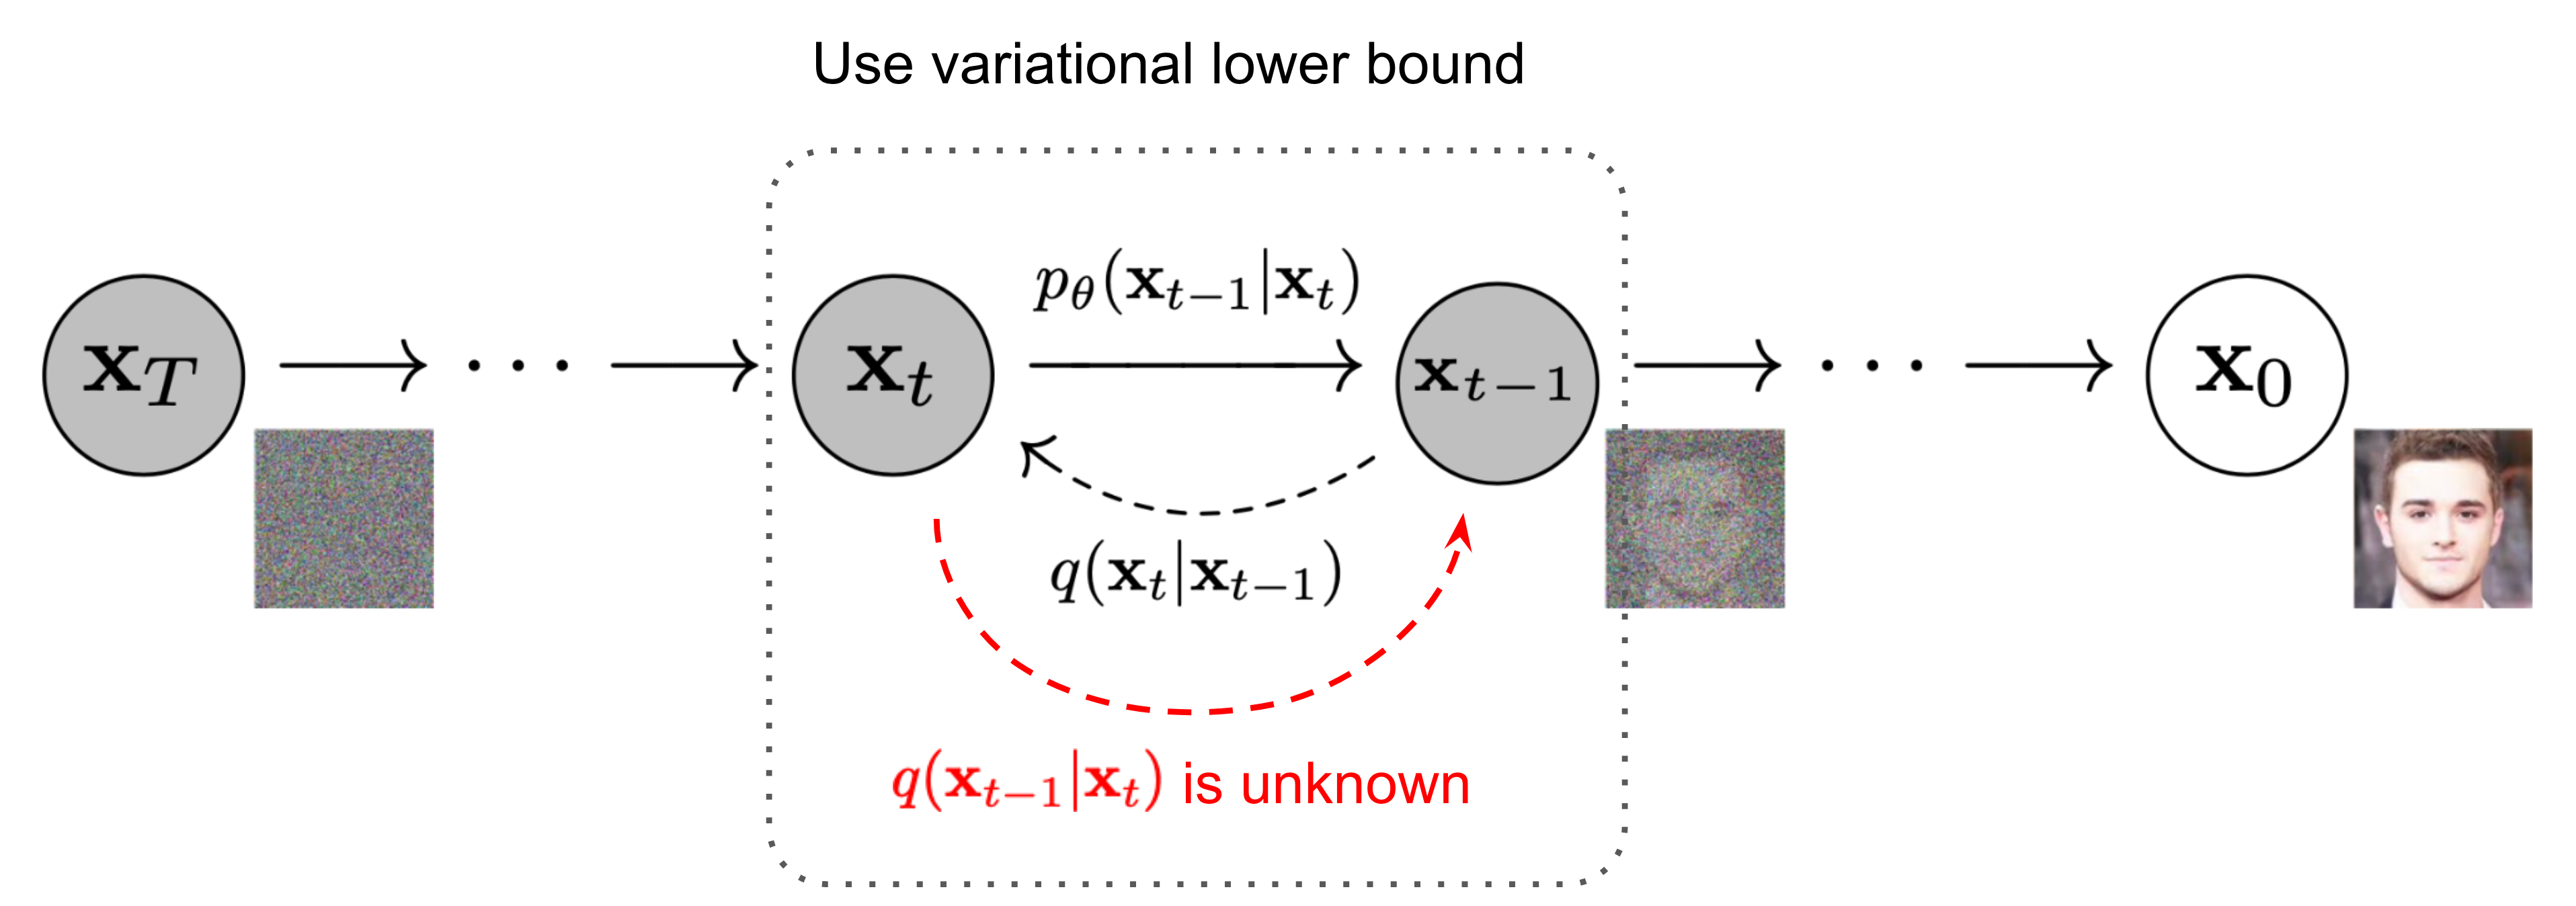
\includegraphics[scale=0.15]{image/DDPM.png}
\caption{DDPM}
\label{fig:DDPM}
\end{figure}

真实数据分布$\mathbf{x}_0 \sim q (\mathbf{x})$，这里的$x_0$可能是$512*512*3$大小的图像集合，也可能是$\mathbb{R}^{n}$中的向量，比如动画BVH解析出的数据表示。

前向扩散过程定义为$T$步的马尔科夫过程，转移概率为$q(\mathbf{x}_t|\mathbf{x}_{t-1}), t \in \mathbb{N}$。对于给定数据$\mathbf{x}_0$，向其添加同维度的高斯样本(微小扰动)，然后递推。设置好每一步添加样本的均值和方差，使得输入样本$x_0$变为标准正太分布的样本，如图4.1所示。比如序列$\left\{\beta_t \in(0,1)\right\}_{t=1}^T, \beta_1 < \beta_2 < \cdots < \beta_T\}$，将转移概率(条件概率)定义为$q\left(\mathbf{x}_t \mid \mathbf{x}_{t-1}\right)=\mathcal{N}\left(\mathbf{x}_t ; \sqrt{1-\beta_t} \mathbf{x}_{t-1}, \beta_t \mathbf{I}\right)$ 当累积信号系数 $\bar\alpha_T\to0$ 时，终端边缘 $q(\mathbf x_T)$ 才趋近标准高斯；单步转移核并不因此变成标准高斯。

令
\begin{equation}
\alpha_t = 1 - \beta_t, \bar{\alpha_{t}} = \prod_{i=1}^{t}\alpha_i.
\end{equation}
对于$q\left(\mathbf{x}_t \mid \mathbf{x}_{t-1}\right)$，由重参数化得
$\mathbf{x}_t =\sqrt{\alpha_t} \mathbf{x}_{t-1}+\sqrt{1-\alpha_t} \epsilon_{t-1}$，
又由高斯分布的叠加特性，可得
$\mathbf{x_0} \rightarrow \mathbf{x_t}$的转化：
\begin{equation}
\begin{array}{rlr}
\mathbf{x}_t & =\sqrt{\alpha_t} \mathbf{x}_{t-1}+\sqrt{1-\alpha_t} \epsilon_{t-1} & \quad ;  \epsilon_{t-1}, \epsilon_{t-2}, \cdots \sim \mathcal{N}(\mathbf{0}, \mathbf{I}) \\
& =\sqrt{\alpha_t \alpha_{t-1}} \mathbf{x}_{t-2}+\sqrt{1-\alpha_t \alpha_{t-1}} \bar{\epsilon}_{t-2}  \\
& =\cdots & \\
& =\sqrt{\bar{\alpha}_t} \mathbf{x}_0+\sqrt{1-\bar{\alpha}_t} \boldsymbol{\epsilon}
\end{array}
\end{equation}
其中合并的高斯分布$\bar{\epsilon}_{t-2} = [\sqrt{\alpha_t(1-\alpha_{t-1})}\epsilon_{t-2}+\sqrt{1-\alpha_t}\epsilon_{t-1}]/\sqrt{1-\alpha_t\alpha_{t-1}}$，归一化后仍为标准高斯。
于是得到
\begin{equation}
q\left(\mathbf{x}_t \mid \mathbf{x}_0\right)=\mathcal{N}\left(\mathbf{x}_t ; \sqrt{\bar{\alpha}_t} \mathbf{x}_0,\left(1-\bar{\alpha}_t\right) \mathbf{I}\right)
\end{equation}
根据变换关系，有$\bar{\alpha_1} > \cdots > \bar{\alpha_T}$。

前向过程：人为设计一个马尔科夫扩散过程，将任意分布(有限维度)，在有限步数之内，逼近一个标准正太分布。

关于DL的建模，可以简单理解为将目标转化特定的语言体系，然后在该体系中构建一个闭环，而且需要梳理一下闭环中的链接关系，并在优化中把这些关系体现出来。

这里的任务是生成训练数据对应空间的样本，由贝叶斯定理，
只要知道$q(\mathbf{x}_t \mid \mathbf{x}_{t-1}), t=1,\cdots, T$整个链条闭环就有了。首先数据的分布$q(\mathbf{x}_0)$是未知的，
且数据分布是我们的目标，但我们会准备很多数据，所以可以假想$q(\mathbf{x}_0)$已知，又前向是已知的，于是，整个链条中，
只剩下反向$q(\mathbf{x}_{t-1} \mid \mathbf{x}_t)$，可用参数模型$\mathcal{N}\left(\mathbf{x}_{t-1} ;
 \boldsymbol{\mu}_\theta\left(\mathbf{x}_t, t\right), \boldsymbol{\Sigma}_\theta\left(\mathbf{x}_t, t\right)\right)$来表示。

前向和反向的闭环，前向：
\begin{equation}
q\left(\mathbf{x}_0, \mathbf{x}_1, \cdots, \mathbf{x}_T\right)=q(\mathbf{x}_{0:T}):=q\left(\mathbf{x}_0\right) \prod_{t=1}^T q\left(\mathbf{x}_t \mid \mathbf{x}_{t-1}\right)
\end{equation}
反向：
\begin{equation}
p_\theta\left(\mathbf{x}_0, \mathbf{x}_1, \cdots, \mathbf{x}_T\right)=p_\theta(\mathbf{x}_{0:T}):=p\left(\mathbf{x}_T\right) \prod_{t=1}^T p_\theta\left(\mathbf{x}_{t-1} \mid \mathbf{x}_t\right)
\end{equation}
这两者都定义了整条轨迹的联合分布，但并不会自动相等；学习的目标是让反向模型尽量逼近前向过程所定义的联合分布。
要优化这两分布，就要找一个刻画两分布的距离的函数。其中KL散度，交叉熵，Stein's score函数均可。
对于KL散度，有
\begin{equation}
\label{orig:path-kl}
\begin{aligned}
& \quad \mathbf{KL}\left(q\left(\mathbf{x}_0, \mathbf{x}_1, \cdots, \mathbf{x}_T\right) \| p_\theta\left(\mathbf{x}_0, \mathbf{x}_1, \cdots, \mathbf{x}_T\right)\right) \\
& \stackrel{(i)}{=}-\mathbb{E}_{q\left(\mathbf{x}_0, \mathbf{x}_1, \cdots, \mathbf{x}_T\right)}\left[\log p_\theta\left(\mathbf{x}_0, \mathbf{x}_1, \cdots, \mathbf{x}_T\right)\right]+\mathbf{const} \\
& \stackrel{(i i)}{=} \underbrace{\mathbb{E}_{q\left(\mathbf{x}_0, \mathbf{x}_1, \cdots, \mathbf{x}_T\right)}\left[-\log p\left(\mathbf{x}_T\right)-\sum_{t=1}^T \log \frac{p_\theta\left(\mathbf{x}_{t-1} \mid \mathbf{x}_t\right)}{q\left(\mathbf{x}_t \mid \mathbf{x}_{t-1}\right)}\right]}_{:=L_{\mathbf{VLB}}}+\mathbf{const} \\
& \stackrel{(i i i)}{\geq} \mathbb{E}\left[-\log p_\theta\left(\mathbf{x}_0\right)\right]+\text { const, }
\end{aligned}
\end{equation}

这里仍沿用前文的符号约定：最大化 ELBO，等价于最小化负 ELBO；后者在下面记为 $L_{\rm VLB}$。阅读其它资料时，应以具体公式的正负号为准。

从式\eqref{orig:path-kl}的推导中看到
\begin{equation}
\log \frac{p_\theta\left(\mathbf{x}_{t-1} \mid \mathbf{x}_t\right)}{q\left(\mathbf{x}_t \mid \mathbf{x}_{t-1}\right)}
\end{equation}
是关键。这里前向$q(\mathbf{x}_t \mid \mathbf{x}_{t-1})$均值、方差已知，而逆向我们假设也满足高斯分布，
利用网络$\mathbf{s}_\theta(\mathbf{x}_t, t)$来表示它。当前情况可以做优化，但是实际没有选择这个，而是考虑到前向的马尔可夫性，
有$q(\mathbf{x}_t \mid \mathbf{x}_{t-1})=q(\mathbf{x}_t \mid \mathbf{x}_{t-1}, x_0)$，然后利用贝叶斯法则，
将三元组$(\mathbf{x}_0, \mathbf{x}_t, \mathbf{x}_{t-1})$做个逆向变形，得到$q(\mathbf{x}_{t-1} \mid \mathbf{x}_t,\mathbf{x}_0)$
的具体计算表达式。然后相关的式子都有表达式，于是可以对$q(\mathbf{x}_t \mid \mathbf{x}_{t-1}, x_0)=q(\mathbf{x}_t \mid \mathbf{x}_{t-1})$
做等量替换。细节如下：
\begin{equation}
\begin{aligned}
q\left(\mathbf{x}_{t-1} \mid \mathbf{x}_t, \mathbf{x}_0\right) & =q\left(\mathbf{x}_t \mid \mathbf{x}_{t-1}, \mathbf{x}_0\right) \frac{q\left(\mathbf{x}_{t-1} \mid \mathbf{x}_0\right)}{q\left(\mathbf{x}_t \mid \mathbf{x}_0\right)} \\
& \propto \exp \left(-\frac{1}{2}\left(\frac{\left(\mathbf{x}_t-\sqrt{\alpha_t} \mathbf{x}_{t-1}\right)^2}{\beta_t}+\frac{\left(\mathbf{x}_{t-1}-\sqrt{\bar{\alpha}_{t-1}} \mathbf{x}_0\right)^2}{1-\bar{\alpha}_{t-1}}-\frac{\left(\mathbf{x}_t-\sqrt{\bar{\alpha}_t} \mathbf{x}_0\right)^2}{1-\bar{\alpha}_t}\right)\right) \\
& =\exp \left(-\frac{1}{2}\left(\frac{\mathbf{x}_t^2-2 \sqrt{\alpha_t} \mathbf{x}_t \mathbf{x}_{t-1}+\alpha_t \mathbf{x}_{t-1}^2}{\beta_t}+\frac{\mathbf{x}_{t-1}^2-2 \sqrt{\bar{\alpha}_{t-1}} \mathbf{x}_0 \mathbf{x}_{t-1}+\bar{\alpha}_{t-1} \mathbf{x}_0^2}{1-\bar{\alpha}_{t-1}}-\frac{\left(\mathbf{x}_t-\sqrt{\bar{\alpha}_t} \mathbf{x}_0\right)^2}{1-\bar{\alpha}_t}\right)\right) \\
& =\exp \left(-\frac{1}{2}\left(\left(\frac{\alpha_t}{\beta_t}+\frac{1}{1-\bar{\alpha}_{t-1}}\right) \mathbf{x}_{t-1}^2-\left(\frac{2 \sqrt{\alpha_t}}{\beta_t} \mathbf{x}_t+\frac{2 \sqrt{\bar{\alpha}_{t-1}}}{1-\bar{\alpha}_{t-1}} \mathbf{x}_0\right) \mathbf{x}_{t-1}+C\left(\mathbf{x}_t, \mathbf{x}_0\right)\right)\right)
\end{aligned}
\end{equation}
其中$C\left(\mathbf{x}_t, \mathbf{x}_0\right)$是和$\mathbf{x}_{t-1}$无关的量，$\propto $表示前面的比例项去掉了，从上面看到，对于逆向的某一步，增加初始数据$\mathbf{x}_0$的条件下，仍然是一个高斯分布，且能计算。
也即
\begin{equation}
q\left(\mathbf{x}_{t-1} \mid \mathbf{x}_t, \mathbf{x}_0\right)=\mathcal{N}\left(\mathbf{x}_{t-1} ; \tilde{\boldsymbol{\mu}}\left(\mathbf{x}_t, \mathbf{x}_0\right), \tilde{\beta}_t \mathbf{I}\right)
\end{equation}
其中$\tilde{\beta}_t=1 /\left(\frac{\alpha_t}{\beta_t}+\frac{1}{1-\bar{\alpha}_{t-1}}\right)=1 /\left(\frac{\alpha_t-\bar{\alpha}_t+\beta_t}{\beta_t\left(1-\bar{\alpha}_{t-1}\right)}\right)=\frac{1-\bar{\alpha}_{t-1}}{1-\bar{\alpha}_t} \cdot \beta_t$

\begin{equation}
\begin{aligned}
\tilde{\boldsymbol{\mu}}_t\left(\mathbf{x}_t, \mathbf{x}_0\right) & =\left(\frac{\sqrt{\alpha_t}}{\beta_t} \mathbf{x}_t+\frac{\sqrt{\bar{\alpha}_{t-1}}}{1-\bar{\alpha}_{t-1}} \mathbf{x}_0\right) /\left(\frac{\alpha_t}{\beta_t}+\frac{1}{1-\bar{\alpha}_{t-1}}\right) \\
& =\left(\frac{\sqrt{\alpha_t}}{\beta_t} \mathbf{x}_t+\frac{\sqrt{\bar{\alpha}_{t-1}}}{1-\bar{\alpha}_{t-1}} \mathbf{x}_0\right) \frac{1-\bar{\alpha}_{t-1}}{1-\bar{\alpha}_t} \cdot \beta_t \\
& =\frac{\sqrt{\alpha_t}\left(1-\bar{\alpha}_{t-1}\right)}{1-\bar{\alpha}_t} \mathbf{x}_t+\frac{\sqrt{\bar{\alpha}_{t-1}} \beta_t}{1-\bar{\alpha}_t} \mathbf{x}_0
\end{aligned}
\end{equation}
将前向过程$\mathbf{x}_0$和$\mathbf{x}_t$的关系代入，得到
\begin{equation}
\begin{aligned}
\tilde{\boldsymbol{\mu}}_t & =\frac{\sqrt{\alpha_t}\left(1-\bar{\alpha}_{t-1}\right)}{1-\bar{\alpha}_t} \mathbf{x}_t+\frac{\sqrt{\bar{\alpha}_{t-1}} \beta_t}{1-\bar{\alpha}_t} \frac{1}{\sqrt{\bar{\alpha}_t}}\left(\mathbf{x}_t-\sqrt{1-\bar{\alpha}_t} \epsilon_t\right) \\
& =\frac{1}{\sqrt{\alpha_t}}\left(\mathrm{x}_t-\frac{1-\alpha_t}{\sqrt{1-\bar{\alpha}_t}} \epsilon_t\right)
\end{aligned}
\end{equation}

而这个时候，只需要将优化目标\eqref{orig:path-kl}的 $ii$ 项中的$q(\mathbf{x}_t \mid \mathbf{x}_{t-1})$
通过贝叶斯公式改写为含 $q(\mathbf{x}_{t-1}\mid\mathbf{x}_t,\mathbf{x}_0)$ 的项，并将边缘比值连乘相消，即得到最终可计算的优化目标。

具体如下：
\begin{equation}
\begin{aligned}
& L_{\mathrm{VLB}}=\mathbb{E}_{q\left(\mathbf{x}_{0: T}\right)}\left[\log \frac{q\left(\mathbf{x}_{1: T} \mid \mathbf{x}_0\right)}{p_\theta\left(\mathbf{x}_{0: T}\right)}\right] \\
& =\mathbb{E}_q\left[\log \frac{\prod_{t=1}^T q\left(\mathbf{x}_t \mid \mathbf{x}_{t-1}\right)}{p_\theta\left(\mathbf{x}_T\right) \prod_{t=1}^T p_\theta\left(\mathbf{x}_{t-1} \mid \mathbf{x}_t\right)}\right] \\
& =\mathbb{E}_q\left[-\log p_\theta\left(\mathbf{x}_T\right)+\sum_{t=1}^T \log \frac{q\left(\mathbf{x}_t \mid \mathbf{x}_{t-1}\right)}{p_\theta\left(\mathbf{x}_{t-1} \mid \mathbf{x}_t\right)}\right] \\
& =\mathbb{E}_q\left[-\log p_\theta\left(\mathbf{x}_T\right)+\sum_{t=2}^T \log \frac{q\left(\mathbf{x}_t \mid \mathbf{x}_{t-1}\right)}{p_\theta\left(\mathbf{x}_{t-1} \mid \mathbf{x}_t\right)}+\log \frac{q\left(\mathbf{x}_1 \mid \mathbf{x}_0\right)}{p_\theta\left(\mathbf{x}_0 \mid \mathbf{x}_1\right)}\right] \\
& =\mathbb{E}_q\left[-\log p_\theta\left(\mathbf{x}_T\right)+\sum_{t=2}^T \log \left(\frac{q\left(\mathbf{x}_{t-1} \mid \mathbf{x}_t, \mathbf{x}_0\right)}{p_\theta\left(\mathbf{x}_{t-1} \mid \mathbf{x}_t\right)} \cdot \frac{q\left(\mathbf{x}_t \mid \mathbf{x}_0\right)}{q\left(\mathbf{x}_{t-1} \mid \mathbf{x}_0\right)}\right)+\log \frac{q\left(\mathbf{x}_1 \mid \mathbf{x}_0\right)}{p_\theta\left(\mathbf{x}_0 \mid \mathbf{x}_1\right)}\right] \\
& =\mathbb{E}_q\left[-\log p_\theta\left(\mathbf{x}_T\right)+\sum_{t=2}^T \log \frac{q\left(\mathbf{x}_{t-1} \mid \mathbf{x}_t, \mathbf{x}_0\right)}{p_\theta\left(\mathbf{x}_{t-1} \mid \mathbf{x}_t\right)}+\sum_{t=2}^T \log \frac{q\left(\mathbf{x}_t \mid \mathbf{x}_0\right)}{q\left(\mathbf{x}_{t-1} \mid \mathbf{x}_0\right)}+\log \frac{q\left(\mathbf{x}_1 \mid \mathbf{x}_0\right)}{p_\theta\left(\mathbf{x}_0 \mid \mathbf{x}_1\right)}\right] \\
& =\mathbb{E}_q\left[-\log p_\theta\left(\mathbf{x}_T\right)+\sum_{t=2}^T \log \frac{q\left(\mathbf{x}_{t-1} \mid \mathbf{x}_t, \mathbf{x}_0\right)}{p_\theta\left(\mathbf{x}_{t-1} \mid \mathbf{x}_t\right)}+\log \frac{q\left(\mathbf{x}_T \mid \mathbf{x}_0\right)}{q\left(\mathbf{x}_1 \mid \mathbf{x}_0\right)}+\log \frac{q\left(\mathbf{x}_1 \mid \mathbf{x}_0\right)}{p_\theta\left(\mathbf{x}_0 \mid \mathbf{x}_1\right)}\right] \\
& =\mathbb{E}_q\left[\log \frac{q\left(\mathbf{x}_T \mid \mathbf{x}_0\right)}{p_\theta\left(\mathbf{x}_T\right)}+\sum_{t=2}^T \log \frac{q\left(\mathbf{x}_{t-1} \mid \mathbf{x}_t, \mathbf{x}_0\right)}{p_\theta\left(\mathbf{x}_{t-1} \mid \mathbf{x}_t\right)}-\log p_\theta\left(\mathbf{x}_0 \mid \mathbf{x}_1\right)\right] \\
& =\mathbb{E}_q[\underbrace{D_{\mathrm{KL}}\left(q\left(\mathbf{x}_T \mid \mathbf{x}_0\right) \| p_\theta\left(\mathbf{x}_T\right)\right)}_{L_T}+\sum_{t=2}^T \underbrace{D_{\mathrm{KL}}\left(q\left(\mathbf{x}_{t-1} \mid \mathbf{x}_t, \mathbf{x}_0\right) \| p_\theta\left(\mathbf{x}_{t-1} \mid \mathbf{x}_t\right)\right)}_{L_{t-1}} \underbrace{-\log p_\theta\left(\mathbf{x}_0 \mid \mathbf{x}_1\right)}_{L_0}] \\
&
\end{aligned}
\end{equation}
看起来比较长，其实非常简单，核心就是第4个等式到第5个等式的变换，变换是根据建模的基本假设来做的，容易想到。上面的KL散度是
关于两个高斯分布的散度，且取了对数，容易得到，损失函数是关于高斯分布均值的平方差的式子(令方差为常数)。
从DL的角度来说，只需让模型预测每一步的均值即可，也即
\begin{equation}
p_\theta(\mathbf x_{t-1}\mid\mathbf x_t)=\mathcal{N}\left(\mathbf{x}_{t-1} ; \frac{1}{\sqrt{\alpha_t}}\left(\mathbf{x}_t-\frac{1-\alpha_t}{\sqrt{1-\bar{\alpha}_t}} \boldsymbol{\epsilon}_\theta\left(\mathbf{x}_t, t\right)\right), \mathbf{\Sigma}_\theta\left(\mathbf{x}_t, t\right)\right)
\end{equation}
其中$\boldsymbol{\epsilon}_\theta\left(\mathbf{x}_t, t\right)$表示神经网络。
进一步选择重新加权的简化训练目标，得到
\begin{equation}
\begin{aligned}
L_t^{\text {simple }} & =\mathbb{E}_{t \sim[1, T], \mathbf{x}_0, \epsilon_t}\left[\left\|\boldsymbol{\epsilon}_t-\boldsymbol{\epsilon}_\theta\left(\mathbf{x}_t, t\right)\right\|^2\right] \\
& =\mathbb{E}_{t \sim[1, T], \mathbf{x}_0, \epsilon_t}\left[\left\|\boldsymbol{\epsilon}_t-\boldsymbol{\epsilon}_\theta\left(\sqrt{\bar{\alpha}_t} \mathbf{x}_0+\sqrt{1-\bar{\alpha}_t} \epsilon_t, t\right)\right\|^2\right]
\end{aligned}
\end{equation}
从中可以看到，只需要预测所有前向步骤所添加的噪声。最终得到训练和推理算法如下：
\begin{figure}[h!]
\centering
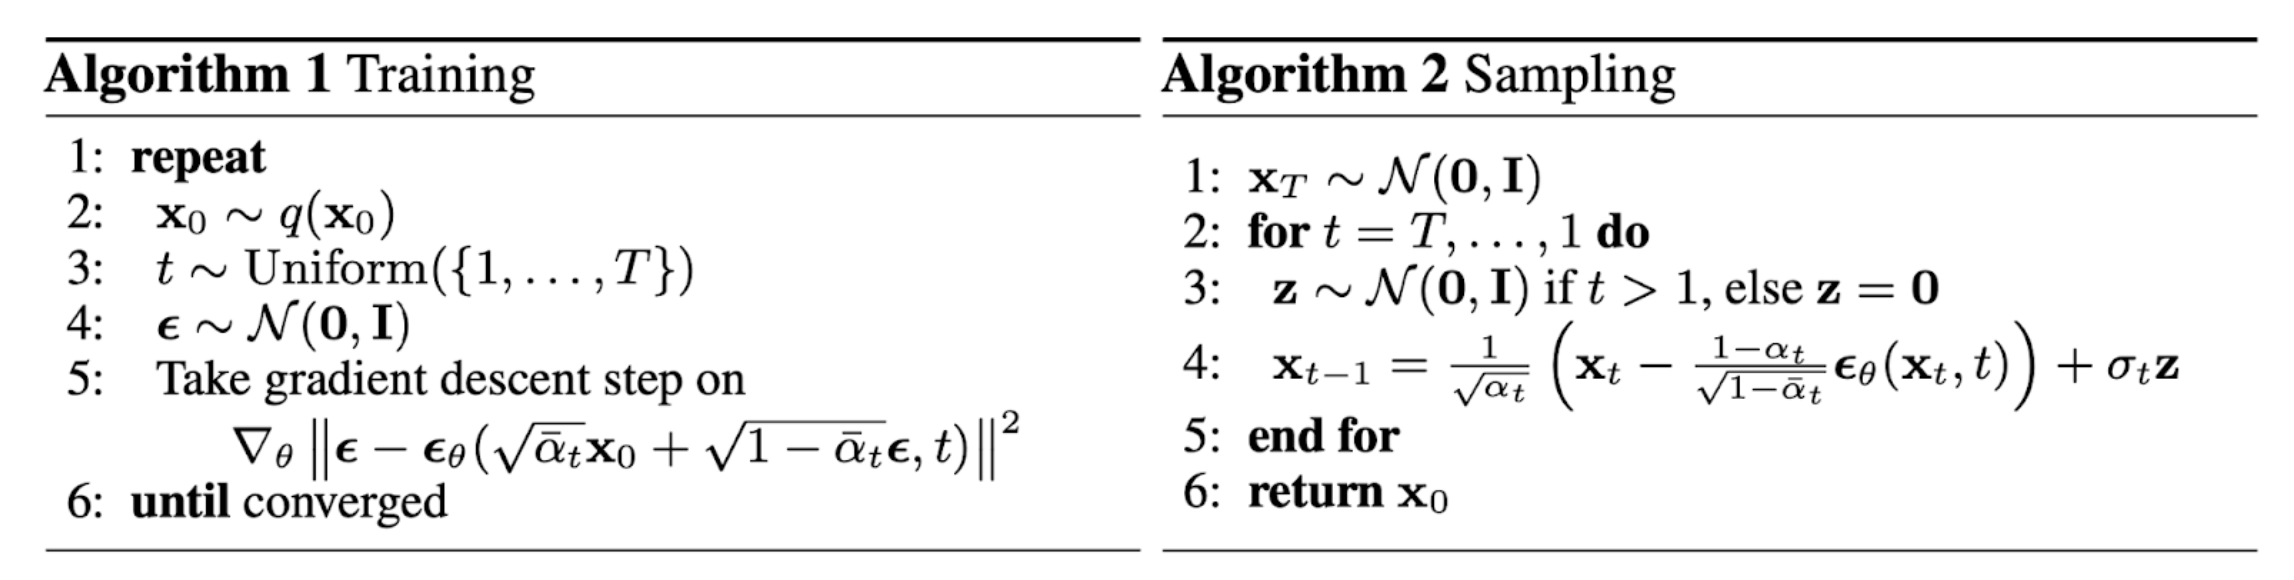
\includegraphics[scale=0.3]{image/DDPM-algo.png}
\caption{DDPM algo}
\label{fig:DDPM-algo}
\end{figure}

这里还有两点需要从上面的推导中单独拎出来。
第一，能够配方算出的，是给定 $\mathbf x_0$ 的
$q(\mathbf x_{t-1}\mid\mathbf x_t,\mathbf x_0)$。
训练时原始样本已知，可以用它计算监督；生成时只知道当前 $\mathbf x_t$，
不能把这个带有干净条件的后验直接当作可执行的逆过程。
网络正是在学习用 $\mathbf x_t,t$ 代替未知干净条件的影响。

第二，固定反向方差 $\nu_t^2I$ 后，两个高斯的 KL 中与均值有关的部分是
\[
\frac1{2\nu_t^2}\|\tilde\mu_t-\mu_\theta(\mathbf x_t,t)\|^2.
\]
把前面得到的均值表达代进去，变为
\[
\frac{\beta_t^2}{2\nu_t^2\alpha_t(1-\bar\alpha_t)}
\|\epsilon-\epsilon_\theta(\mathbf x_t,t)\|^2.
\]
因此，最后常用的无权重噪声 MSE 是一种重新加权。
它便于训练，但不能说时间相关系数在数学上都不影响优化。
如果所有时间步共用同一组参数，不同权重会改变各个噪声级争取模型容量的方式。

再回到采样。均值网络算出 $\mu_\theta$ 后，通常还要执行
$\mathbf x_{t-1}=\mu_\theta(\mathbf x_t,t)+\nu_t z$。
这里重新抽取的 $z$，与训练时用来构造 $\mathbf x_t$ 的噪声标签不是同一个对象。
这就把“前向加噪得到训练对”“回归逆过程参数”“执行逆过程生成”三步接上了。
下面换到 NCSN 的分数视角时，这条关系还会出现。\cite{ddpm,theorybook}



\section{NCSN}

% \begin{itemize}
%     \item Langevin MCMC 
%     \item  ancestral sampling
%     \item  
% \end{itemize}

% generalize  Perturbing data with multiple noise scales to infinite number of noise scales,
% 把系列离散扰动数据的分布连续化为能用随机微分方程来刻画。

% 把任意数据分布映射到先验分布（高斯分布）。

% SMLD的离散化：

% DDPM的离散化：

% 如何训练一个时间相关的分数模型：

% \begin{equation}
% \boldsymbol{\theta}^*=\underset{\boldsymbol{\theta}}{\arg \min } \mathbb{E}_t\left\{\lambda(t) \mathbb{E}_{\mathbf{x}(0)} \mathbb{E}_{\mathbf{x}(t) \mid \mathbf{x}(0)}\left[\left\|\mathbf{s}_{\boldsymbol{\theta}}(\mathbf{x}(t), t)-\nabla_{\mathbf{x}(t)} \log p_{0 t}(\mathbf{x}(t) \mid \mathbf{x}(0))\right\|_2^2\right]\right\}
% \end{equation}

% 概率流联系常微分的数值解：reverse-time SDE存在一个对应的ODE数值解法。对任意的扩散过程，存在一个确定的过程，其迹和SDE的边缘概率密度分布一致。该确定过程能用如下ODE刻画：
% \begin{equation}
% \mathbf{d} \mathbf{x}=\left[\mathbf{f}(\mathbf{x}, t)-\frac{1}{2} g(t)^2 \nabla_{\mathbf{x}} \log p_t(\mathbf{x})\right] \mathbf{d} t
% \end{equation}
% 该方程被称为：probability flow ODE。
% 该常微分方程的解迹在$t$处的采样样本的概率密度为$p_{t}(x)$。

% 令$\mathbf{f}(\mathbf{x}, t)=\mathbf{0}, g(t)=\sqrt{2t}$，(此时，$p_t(\mathbf{x})=p_{\text {data }}(\mathbf{x}) \otimes \mathcal{N}\left(\mathbf{0}, t^2 \boldsymbol{I}\right)$，其中$\otimes$表示卷积，分数模型$s_\phi(\mathbf{x}, t) \approx \nabla \log p_t(\mathbf{x})$)，
% 得到 经验 PF ODE：

% \begin{equation}
% \frac{\mathbf{d} \mathbf{x}_t}{\mathbf{~d} t}=-t s_\phi\left(\mathbf{x}_t, t\right)
% \end{equation}
% $X_T$初始化，用欧拉或Heun法求解得到解迹：$\left\{\hat{\mathbf{x}}_t\right\}_{t \in[0, T]}$。$t=0$符合$p_{data}(\mathbf{x})$。 将图像映射到$[-1,1]$后，设置$T=80, s=0.002$，$s$是采样步长。

% 条件逆扩散：
% \begin{equation}
% \mathbf{d} \mathbf{x}=\left\{\mathbf{f}(\mathbf{x}, t)-g(t)^2\left[\nabla_{\mathbf{x}} \log p_t(\mathbf{x})+\nabla_{\mathbf{x}} \log p_t(\mathbf{y} \mid \mathbf{x})\right]\right\} \mathbf{d} t+g(t) \mathbf{d} \overline{\mathbf{w}}
% \end{equation}

数据样本$\left\{\mathbf{x}_i \in \mathbb{R}^D\right\}_{i=1}^N$ 满足独立同分布，数据的分布用$p_{data}(\mathbf{x})$表示，概率密度$p(\mathbf{x})$的分数定义为$\nabla_{\mathbf{x}} \log p(\mathbf{x})$，分数网络score network $s_{\theta}:\mathbb{R}^D \rightarrow \mathbb{R}^D$，其中$\theta$表示网络参数。用分数网络来刻画数据分布，因为若概率密度的分数已知，则可以利用郎之万动力采样，其采样出的数据符合数据原始分布。 因此基于分数的生成模型的核心，就是分数匹配和郎之万动力采样。

能量模型定义为：
\begin{equation}
p_m(\mathbf{x} ; \boldsymbol{\theta})=\frac{\tilde{p}_m(\mathbf{x} ; \boldsymbol{\theta})}{Z_{\boldsymbol{\theta}}}, \quad Z_{\boldsymbol{\theta}}=\int \tilde{p}_m(\mathbf{x} ; \boldsymbol{\theta}) \mathrm{d} \mathbf{x}
\end{equation}
其分数则为：
\begin{equation}
\mathbf{s}_m(\mathbf{x} ; \boldsymbol{\theta}) \triangleq \nabla_{\mathbf{x}} \log p_m(\mathbf{x} ; \boldsymbol{\theta})=\nabla_{\mathbf{x}} \log \tilde{p}_m(\mathbf{x} ; \boldsymbol{\theta}), \quad  \mathbf{s}_d(\mathbf{x} ; \boldsymbol{\theta}) \triangleq \nabla_{\mathbf{x}} \log p_d(\mathbf{x} ; \boldsymbol{\theta})
\end{equation}
消去了$Z_{\boldsymbol{\theta}}$，其中$p_d$是$p_{data}$的简写。

若写成 $\tilde p_m(x;\theta)=\exp[-E_\theta(x)]$，就得到常见的能量形式，
空间分数为 $-\nabla_xE_\theta(x)$。这里消去的是对 $x$ 求导时的归一化常数，
对参数求导的极大似然训练仍然会遇到 $Z_\theta$。



上述分数匹配于2005(Hyvärinen, 2005)年被提出，主要用来解决基于能量的概率密度估计(极大似然建模)分母归一化因子难处理的问题，原始优化目标为：
\begin{equation}
\frac{1}{2} \mathbb{E}_{p_{\text {data }}}\left[\left\|\mathbf{s}_{\boldsymbol{\theta}}(\mathbf{x})-\nabla_{\mathbf{x}} \log p_{\text {data }}(\mathbf{x})\right\|_2^2\right]
\end{equation}
该论文得出其等价形式：
\begin{equation}
\label{orig:score-loss}
J(\boldsymbol{\theta}) \triangleq \mathbb{E}_{p_d}\left[\operatorname{tr}\left(\nabla_{\mathbf{x}} \mathbf{s}_m(\mathbf{x} ; \boldsymbol{\theta})\right)+\frac{1}{2}\left\|\mathbf{s}_m(\mathbf{x} ; \boldsymbol{\theta})\right\|_2^2\right],
\end{equation}
其中$tr$表示矩阵的迹，上述公式需要计算 log-density的Hessian矩阵，计算量非常大。

在数学上，1981年就有了相关定理。参考数学基础部分。

Sliced Score Matching一文对(Hyvärinen, 2005)做了改进，
得出
\begin{equation}
\mathbb{E}_{p_{\mathbf{v}}} \mathbb{E}_{p_{\text {data }}}\left[\mathbf{v}^{\top} \nabla_{\mathbf{x}} \mathbf{s}_{\boldsymbol{\theta}}(\mathbf{x}) \mathbf{v}+\frac{1}{2}\left\|\mathbf{s}_{\boldsymbol{\theta}}(\mathbf{x})\right\|_2^2\right]
\end{equation}
其中$p_{\mathbf{v}}$是一个简单分布的随机向量，比如多元标准高斯分布。该结论表明，将原始高维矩阵关于随机向量做投影，去逼近式\eqref{orig:score-loss}中的迹，能减少计算量的同时，保持无偏估计。

另外，2011年的文章 A Connection Between Score Matching and Denoising Autoencoders 提出的去噪分数匹配，避免了损失中对分数网络输入求导的迹计算；网络参数仍需正常反向传播。它估计的是扰动后的数据分数。具体来说，定义扰动后的数据分布为：
\begin{equation}
q_\sigma(\tilde{\mathbf{x}}) \triangleq \int q_\sigma(\tilde{\mathbf{x}} \mid \mathbf{x}) p_{\text {data }}(\mathbf{x}) \mathrm{d} \mathbf{x}
\end{equation}
于是优化目标
\begin{equation}
\frac{1}{2} \mathbb{E}_{q_\sigma(\tilde{\mathbf{x}} \mid \mathbf{x}) p_{\text {data }}(\mathbf{x})}\left[\left\|\mathbf{s}_{\boldsymbol{\theta}}(\tilde{\mathbf{x}})-\nabla_{\tilde{\mathbf{x}}} \log q_\sigma(\tilde{\mathbf{x}} \mid \mathbf{x})\right\|_2^2\right]
\end{equation}
的最优解$\mathbf{s}_{\boldsymbol{\theta}^*}(\mathbf{x})$当扰动很小的时候，有：
\begin{equation}
\mathbf{s}_{\boldsymbol{\theta}^*}(\mathbf{x})=\nabla_{\mathbf{x}} \log q_\sigma(\mathbf{x}) \approx \nabla_{\mathbf{x}} \log p_{\text {data }}(\mathbf{x})
\end{equation}

朗之万动力学在已知分数函数$\nabla_{\mathbf{x}} \log p(\mathbf{x})$的情况下，可以采样出概率密度为$p(\mathbf{x})$的样本。
具体来说：
\begin{equation}
\label{orig:langevin}
\tilde{\mathbf{x}}_t=\tilde{\mathbf{x}}_{t-1}+\frac{\epsilon}{2} \nabla_{\mathbf{x}} \log p\left(\tilde{\mathbf{x}}_{t-1}\right)+\sqrt{\epsilon} \mathbf{z}_t
\end{equation}
其中$\epsilon$表示固定的步长大小，$\tilde{\mathbf{x}}_0 \sim \pi(\mathbf{x})$是一个先验分布，$z_t \sim \mathcal{N}(0, I)$。当$\epsilon \rightarrow 0, T \rightarrow \infty$，在一些正则条件下，$
\tilde{\mathbf{x}}_T \sim p(\mathbf{x})$。
具体分析见：
\href{https://www.stats.ox.ac.uk/~teh/research/compstats/WelTeh2011a.pdf}{Bayesian Learning via Stochastic Gradient Langevin Dynamics 2011}。

NCSN是在以上基础上提出的，作者分析了基于分数的生成模型的两个问题。基于一些基础实验，1：Sliced score matching在原始数据上的迭代损失曲线没添加噪声后的迭代平稳，而且前者是极度不平稳，上下波动很大，对此作者给出了基于流形假设的分析；2.通过分数匹配的方法，去做一个混合高斯分布的分数估计，发现在低密度区域匹配的很不准确，同时混合模型的权重因子失效严重，在混合区域，使用郎之万动力采样，是极度缓慢才能收敛到实际情况，因为分数函数关于不同混合密度的支撑集上的函数值，是和混合因子无关的，导致优化很难处理混合模型各自的连接区域的密度情况，以至于采样不准确。

基于这些基本观察，分析，作者提出了带尺度的扰动分数模型：Noise Conditional Score Networks。一来解决了高低密度不均匀难以优化，导致采样不准的问题，二来解决了数据在高维空间的低维嵌入的普遍现象导致的分数模型无法正确优化的问题。因为将数据不断扰动，能使其充满整个空间，同时，低密度区域得到了有效填充，另外不同尺度，从极小扰动到不断增幅扰动因子，使得一个分数模型在全空间中去拟合不同尺度的扰动，得到非常充分的训练，因此其逆向采样，能更好的近似到原始分布。

称$\mathbf{s}_{\boldsymbol{\theta}}(\mathbf{x}, \sigma)$为Noise Conditional Score Network (NCSN)是指：
设扰动因子$\{\sigma_i\}_{i=1}^{L}$满足$\frac{\sigma_1}{\sigma_2}=\dots=\frac{\sigma_{L-1}}{\sigma_L}>1 $，
定义扰动尺度为$\sigma$的数据分布
\begin{equation}
q_\sigma(\tilde{\mathbf{x}}) \triangleq \int p_{\text {data }}(\mathbb{t}) \mathcal{N}(\tilde{\mathbf{x}} \mid \mathbb{t}, \sigma^2I)\,\mathrm d\mathbb t
\end{equation}
训练一个
\begin{equation}
\forall \sigma \in\left\{\sigma_i\right\}_{i=1}^L: \mathbf{s}_{\boldsymbol{\theta}}(\tilde{\mathbf{x}}, \sigma) \approx \nabla_{\mathbf{x}} \log q_\sigma(\tilde{\mathbf{x}})
\end{equation}
的网络，其中$ \mathbf{x} \in \mathbb{R}^{D}, \mathbf{s}_{\boldsymbol{\theta}} \in \mathbb{R}^{D}$。

因$q_\sigma(\tilde{\mathbf{x}} \mid \mathbf{x})=\mathcal{N}\left(\tilde{\mathbf{x}} \mid \mathbf{x}, \sigma^2 I\right)$，有$\nabla_{\tilde{\mathbf{x}}} \log q_\sigma(\tilde{\mathbf{x}} \mid \mathbf{x})=-(\tilde{\mathbf{x}}-\mathbf{x}) / \sigma^2$，于是对于给定的尺度$\sigma$，其去噪分数匹配损失为：
\begin{equation}
\ell(\boldsymbol{\theta} ; \sigma) \triangleq \frac{1}{2} \mathbb{E}_{p_{\text {data }}(\mathbf{x})} \mathbb{E}_{\tilde{\mathbf{x}} \sim \mathcal{N}\left(\mathbf{x}, \sigma^2 I\right)}\left[\left\|\mathrm{s}_{\boldsymbol{\theta}}(\tilde{\mathbf{x}}, \sigma)+\frac{\tilde{\mathbf{x}}-\mathrm{x}}{\sigma^2}\right\|_2^2\right]
\end{equation}
对于所有尺度$\forall \sigma \in\left\{\sigma_i\right\}_{i=1}^L$得到最终的优化目标：
\begin{equation}
\mathcal{L}\left(\boldsymbol{\theta} ;\left\{\sigma_i\right\}_{i=1}^L\right) \triangleq \frac{1}{L} \sum_{i=1}^L \lambda\left(\sigma_i\right) \ell\left(\boldsymbol{\theta} ; \sigma_i\right)
\end{equation}其中$ \lambda\left(\sigma_i\right)>0$，为依赖于$\sigma_i$的系数函数。

该目标函数的最优解$\mathbf{s}_{\boldsymbol{\theta}^*}(\mathbf{x}, \sigma)$满足
$\forall i \in \{1, 2, \cdots, L \}, \mathbf{s}_{\boldsymbol{\theta}^*}\left(\mathbf{x}, \sigma_i\right)=\nabla_{\mathbf{x}} \log q_{\sigma_i}(\mathbf{x})$。$\lambda(\cdot)$选择使得所有尺度因子的数量级一致，经验得知，一个训练好的分数模型，其范数正比于尺度的倒数，又$\frac{\tilde{\mathbf{x}}-\mathbf{x}}{\sigma} \sim \mathcal{N}(0, I)$，因此，选择$\lambda(\sigma)=\sigma^2$，使得$\left\|\sigma \mathbf{s}_{\boldsymbol{\theta}}(\mathbf{x}, \sigma)\right\|_2 \propto 1$。

最后论文提出了annealed Langevin dynamics采样算法（对比式\eqref{orig:langevin}）：
将原始步长$\epsilon$改进为$\epsilon \cdot \sigma^2_i / \sigma^2_L$。
\begin{figure}[h!]
\centering
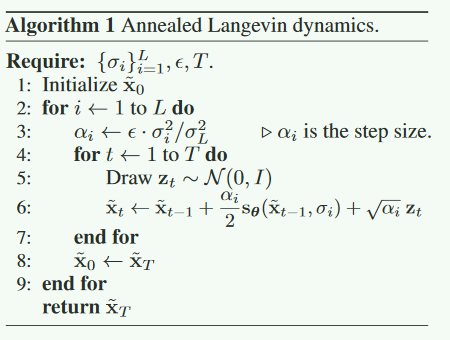
\includegraphics[scale=0.9]{image/NCSNLD.jpg}
\caption{NCSN annealed Langevin dynamics}
\label{fig:NCSN}
\end{figure}

\subsection{score matching}

上面已经列出了分数匹配与去噪分数匹配的目标，这里把它们等价的原因再写一步，
否则容易误以为只是在两个损失之间换了个名字。

先看原始分数匹配。将平方误差展开，唯一含有未知真实分数的交叉项是
\[
-\int p(x)s_\theta(x)^\top\nabla\log p(x)\,\mathrm dx
=-\int s_\theta(x)^\top\nabla p(x)\,\mathrm dx.
\]
在边界项消失时，对每个坐标做分部积分，得到
$\int p(x)\nabla\cdot s_\theta(x)\,\mathrm dx$。
其它关于真实分数的平方项不依赖网络参数，因此得到前面写出的迹与分数平方目标。
这里去掉的是与参数无关的常数，不是随意删掉含有 $\theta$ 的项。

去噪分数匹配再向前走了一步。记扰动边缘为
$q_\sigma(\tilde x)=\int q_\sigma(\tilde x\mid x)p_{\rm data}(x)\,\mathrm dx$，
对 $\tilde x$ 求导并除以 $q_\sigma(\tilde x)$：
\begin{align}
\nabla_{\tilde x}\log q_\sigma(\tilde x)
&=\int\frac{q_\sigma(\tilde x\mid x)p_{\rm data}(x)}{q_\sigma(\tilde x)}
 \nabla_{\tilde x}\log q_\sigma(\tilde x\mid x)\,\mathrm dx\\
&=\mathbb E[\nabla_{\tilde x}\log q_\sigma(\tilde X\mid X)\mid\tilde X=\tilde x].
\end{align}
也就是说，已知条件分数的条件平均，恰好等于我们想学的边缘分数。
而平方回归的最优解正是标签在给定输入下的条件平均，
所以用可计算的条件分数作监督，仍然能够学到未知的边缘分数。

对高斯扰动，条件分数是 $-(\tilde x-x)/\sigma^2$，还可以整理为
\[
\mathbb E[X\mid\tilde X=\tilde x]
=\tilde x+\sigma^2\nabla\log q_\sigma(\tilde x).
\]
这就是此设定下的 Tweedie 公式。分数模型、噪声预测与干净样本估计在这里接了起来。
不过右边给出的是后验均值：噪声很大、一个观测可能对应多个原始样本时，
均值并不一定是其中某个真实样本，更不能由它推断一步就能完成所有生成。\cite{theorybook}



\subsection{极大似然的计算}
Yang Song继其SGM模型，给出了SDE解的边缘分布同数据的分布的KL散度与SM模型优化对象的存在一个不等关系，说明在指定权重与正则条件下，分数匹配误差可控制反向 SDE 的数据分布误差。这个界本身不是逐样本似然的计算公式。

具体来讲：
\begin{equation}
D_{\mathrm{KL}}\left(p \| p_{\boldsymbol{\theta}}^{\mathrm{SDE}}\right) \leq \mathcal{J}_{\mathrm{SM}}\left(\boldsymbol{\theta} ; g(\cdot)^2\right)+D_{\mathrm{KL}}\left(p_T \| \pi\right)
\end{equation}
这里的训练对象仍是分数网络；概率流 ODE 是由它进一步构造的。

在此基础上Cheng Lu等人，给出了扩散对应的ODE的似然函数的上界。
\begin{equation}
\mathcal{J}_{\mathrm{ODE}}(\theta) \leq \sqrt{\mathcal{J}_{\mathrm{SM}}(\theta)} \cdot \sqrt{\mathcal{J}_{\text {Fisher }}(\theta)}
\end{equation}

相关分析表明，一阶分数匹配误差本身不足以无条件控制 ODE 的似然误差；在相应假设下，高阶分数误差也进入控制关系，由此提出高阶去噪分数匹配训练。似然改善与样本质量仍应分别评估。

这里把“似然的计算”和“用什么目标训练”分开一下。
前面的不等式说明：在相应路径正则性与权重设定下，控制分数误差，
可以控制反向 SDE 生成分布的误差；它并没有直接给出每个输入样本的概率密度值。

若使用后面要介绍的概率流 ODE，记其速度为 $v_\theta(x,t)$。
一个小时间步的映射是 $x\mapsto x+h v_\theta(x,t)$，
Jacobian 为 $I+hD_xv_\theta$。利用
$\log\det(I+hD_xv_\theta)=h\operatorname{tr}(D_xv_\theta)+O(h^2)$，
变量替换公式沿轨迹给出
\[
\frac{\mathrm d}{\mathrm dt}\log p_t^\theta(x_t)
=-\nabla\cdot v_\theta(x_t,t).
\]
所以从一个观测 $x_0$ 正向积分到 $x_T$ 后，
\[
\log p_0^\theta(x_0)=\log\pi(x_T)
 +\int_0^T\nabla\cdot v_\theta(x_t,t)\,\mathrm dt.
\]
先验密度可以计算，积分项又由网络向量场决定，这就是计算模型似然的路径。
网络不是完美分数时，仍可在可逆性等条件下定义它所诱导的 ODE 模型密度；
但这个密度是否逼近真实数据，是另一个学习问题。
实际数值积分和随机迹估计也会有误差。

因此，一阶分数训练不是“不能计算 ODE 的似然”，
而是不能仅凭一个很小的一阶训练误差，就无条件保证 ODE 模型的似然误差也很小。
有关高阶分数误差的结果是在附加假设下分析这种控制关系，
不是要求每个可以计算似然的模型都必须另训二阶和三阶网络。\cite{sde,theorybook}



\section{连续版Score SDE}

这一小节沿用原文献的部分符号：下式的 $\alpha_i$ 是累积信号强度，
对应 DDPM 小节的 $\bar\alpha_i$，不是单步 $1-\beta_i$。
NCSN 原先将噪声级按从大到小编号；下面转而按前向加噪时间从小到大编号。
只是索引顺序改变，不是把训练过程改成逐步去噪。


SDE中的噪声尺度因子，和NCSN的写法就大小比较在指标上是相反的，原因在于使用DDPM的方式，重新定义了NCSN中的优化目标，得到
\begin{equation}
\label{orig:discrete-score}
\boldsymbol{\theta}^*=\underset{\boldsymbol{\theta}}{\arg \min } \sum_{i=1}^N\left(1-\alpha_i\right) \mathbb{E}_{p_{\text {data }}(\mathbf{x})} \mathbb{E}_{p_{\alpha_i}(\tilde{\mathbf{x}} \mid \mathbf{x})}\left[\left\|\mathbf{s}_{\boldsymbol{\theta}}(\tilde{\mathbf{x}}, i)-\nabla_{\tilde{\mathbf{x}}} \log p_{\alpha_i}(\tilde{\mathbf{x}} \mid \mathbf{x})\right\|_2^2\right] .
\end{equation}
和逆向马尔科夫链(采样)
\begin{equation}
\mathbf{x}_{i-1}=\frac{1}{\sqrt{1-\beta_i}}\left(\mathbf{x}_i+\beta_i \mathbf{s}_{\boldsymbol{\theta}^*}\left(\mathbf{x}_i, i\right)\right)+\sqrt{\beta_i} \mathbf{z}_i, \quad i=N, N-1, \cdots, 1
\end{equation}
论文中将其称为ancestral sampling。

问题是式\eqref{orig:discrete-score}能通过ELBO推导出来？通过ELBO推导出来，优化的是均值，而转移概率为高斯，对数求导后，差不多也是均值。仔细检查下，应该就是通过ELBO得到式\eqref{orig:discrete-score}所示的分数表达形式。

两者的分数表达形式和采样形式差别不大，将其连续化，并做形式上的推广，得到$It\hat{o}$ SDE方程：
\begin{equation}
\mathrm{d} \mathbf{x}=\mathbf{f}(\mathbf{x}, t) \mathrm{d} t+g(t) \mathrm{d} \mathbf{w}
\end{equation}
而Anderson (1982) 的论文表示，其逆向也是扩散过程， reverse-time SDE为：
\begin{equation}
\mathrm{d} \mathbf{x}=\left[\mathbf{f}(\mathbf{x}, t)-g(t)^2 \nabla_{\mathbf{x}} \log p_t(\mathbf{x})\right] \mathrm{d} t+g(t) \mathrm{d} \overline{\mathbf{w}}
\end{equation}
其对应的优化目标可写为：
\begin{equation}
\boldsymbol{\theta}^*=\underset{\boldsymbol{\theta}}{\arg \min } \mathbb{E}_t\left\{\lambda(t) \mathbb{E}_{\mathbf{x}(0)} \mathbb{E}_{\mathbf{x}(t) \mid \mathbf{x}(0)}\left[\left\|\mathbf{s}_{\boldsymbol{\theta}}(\mathbf{x}(t), t)-\nabla_{\mathbf{x}(t)} \log p_{0 t}(\mathbf{x}(t) \mid \mathbf{x}(0))\right\|_2^2\right]\right\} .
\end{equation}
其中$\lambda:[0, T] \rightarrow \mathbb{R}_{>0}, t\in [0, T], \mathbf{x}(0) \sim p_0(\mathbf{x}), \mathbf{x}_t \sim p_{0t}(\mathbf{x}(t) \mid \mathbf{x}(0))$
其解$\mathbf{s}_{\boldsymbol{\theta}^*}\left(\mathbf{x}, t\right)=\nabla_{\mathbf{x}} \log p_{t}(\mathbf{x})$对几乎所有$\mathbf{x}, t$成立。
另外需要注意的是，对这里预先规定的前向过程，若$\mathbf{f}(\cdot, t)$是仿射的，则转移核是高斯分布。均值和方差能通过相应方程计算出来，参考( Arno Solin 2019)Applied stochastic differential equations。

这里需要注意的是，论文2.1节指出，NCSN尺度上的逆向描述被简写为SMLD(DENOISING SCORE MATCHING WITH LANGEVIN  DYNAMICS)，另外在3.4节，对其做连续化SDE推导的时候，扩散过程也是满足马尔可夫性的。这点和NCSN中从大到小尺度添加噪声训练分数匹配模型NCSN是不同的，其扰动核没有马尔可夫性假设，但是蕴含了马尔科夫性。
具体来说，$p_{\sigma_i}(\mathbf{x} \mid \mathbf{x_0})$对应的$\mathbf{x}_i$满足如下的马尔科夫链：
\begin{equation}
\mathbf{x}_i=\mathbf{x}_{i-1}+\sqrt{\sigma_i^2-\sigma_{i-1}^2} \mathbf{z}_{i-1}, \quad i=1, \cdots, N
\end{equation}
这里方差是$\sigma_i^2-\sigma_{i-1}^2$的原因在于SMLD并不是DDPM那样递归的定义，而是在$\mathbf{x}_0$上，逐级的增加扰动噪声$\mathbf{x}_{\sigma_i}=\mathbf{x}_0+\sigma_i z$，$z\sim\mathcal N(0,I)$。上式连续化得到
\begin{equation}
\mathrm{d} \mathbf{x}=\sqrt{\frac{\mathrm{d}\left[\sigma^2(t)\right]}{\mathrm{d} t}} \mathrm{~d} \mathbf{w} .
\end{equation}
表达了$\{\mathbf{x}(t)\}^{1}_{t=0}$的前向过程的SDE形式。

DDPM的扰动核$\left\{p_{\alpha_i}\left(\mathbf{x} \mid \mathbf{x}_0\right)\right\}_{i=1}^N$
对应的离散马尔科夫链：
\begin{equation}
\mathbf{x}_i=\sqrt{1-\beta_i} \mathbf{x}_{i-1}+\sqrt{\beta_i} \mathbf{z}_{i-1}, \quad i=1, \cdots, N
\end{equation}
当$N \rightarrow \infty$时，收敛到如下SDE：

\begin{equation}
\mathrm{d} \mathbf{x}=-\frac{1}{2} \beta(t) \mathbf{x} \mathrm{d} t+\sqrt{\beta(t)} \mathrm{d} \mathbf{w}
\end{equation}

论文称SMLD的SDE为Variance Exploding (VE) SDE， 称DDPM的SDE为Variance Preserving (VP) SDE， 并给出了 sub-VP SDE：
\begin{equation}
\mathrm{d} \mathbf{x}=-\frac{1}{2} \beta(t) \mathbf{x} \mathrm{d} t+\sqrt{\beta(t)\left(1-e^{-2 \int_0^t \beta(s) \mathrm{d} s}\right)} \mathrm{d} \mathbf{w}
\end{equation}其在似然函数的计算上更加准确。

当得到分数模型后，就可以利用reverse-time SDE 采样得到生成样本。数值求解器也可以提供来自SDEs的近似轨迹，比如Euler-Maruyama，Runge-Kutta methods等方法，可以用来求解reverse-time SDE，获得生成样本。
另外DDPM的祖先采样法，不能用在VE SDE，作者这里提出了reverse diffusion samplers，具体分析细节可看附录E部分。因为这里有训练好的分数模型，有利于求解，而分数模型有对应的郎之万MCMC采样，因此作者综合考虑这些特性，给出了Predictor-Corrector(PC) samplers 采样器，其结合了分数模型的采样特点，也考虑了SDE的数值求解，同时也考虑了DDPM等的采样方法。
细节见附录部分。
\begin{figure}[h!]
\centering
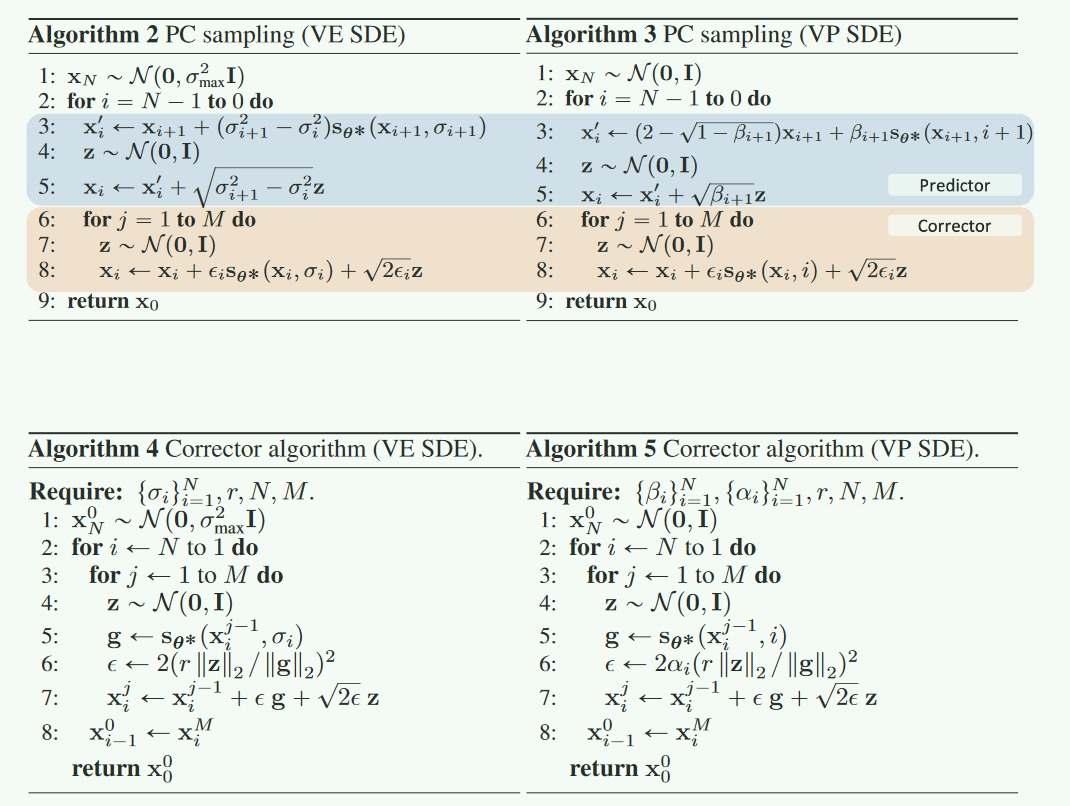
\includegraphics[scale=0.5]{image/PredictorCorrector.jpg}
\caption{SDE Predictor Corrector}
\label{fig:PC}
\end{figure}

另外SDE有对应的常微分方程，
\begin{equation}
\mathrm{d} \mathbf{x}=\left[\mathbf{f}(\mathbf{x}, t)-\frac{1}{2} g(t)^2 \nabla_{\mathbf{x}} \log p_t(\mathbf{x})\right] \mathrm{d} t
\end{equation}
该常微分方程的解，保持SDE所有边缘分布，且构成是确定的。作者将其称为probability flow ODE。当分析模型得到恰当的训练后，它就是一个neural network(Neural Ordinary Differential Equations)，且能用来精确的计算数据(在量化的意义下)的似然值。这块内容在“极大似然的计算”章节中细讲。
% \subsection{stochastic gradient Langevin dynamics}

为什么上式恰好多出一个 $1/2$，可以直接用前面已经推导的 Fokker--Planck 方程看出来。
在扩散系数只依赖时间、且各方向相同的情形，原 SDE 的密度满足
\[
\partial_t p_t=-\nabla\cdot(\mathbf f p_t)+\tfrac12g(t)^2\Delta p_t.
\]
因为 $\nabla p_t=p_t\nabla\log p_t$，扩散项也可以写成散度：
\[
\partial_t p_t=-\nabla\cdot\left[
 p_t\left(\mathbf f-\tfrac12g(t)^2\nabla\log p_t\right)\right].
\]
这已经是一个确定性速度场的连续性方程。
所以，在精确分数和匹配的初始分布等条件下，
这个速度场驱动的 ODE 与原 SDE 具有相同的逐时边缘密度。
系数 $1/2$ 来自扩散通量的改写，不是把反向 SDE 的噪声项简单删掉。

还需要留意时间的方向。前面 reverse-time SDE 的写法仍使用原来的 $t$，
生成时 $t$ 从 $T$ 走向0，$\mathrm dt$ 为负。
若另设 $r=T-t$，把它改写成正步长过程，漂移应写为
\[
\mathrm dY_r=\left[-\mathbf f(Y_r,T-r)+g(T-r)^2s_\theta(Y_r,T-r)\right]\mathrm dr
 +g(T-r)\mathrm dB_r.
\]
这两种时钟描述同一个逆向过程，不能只把步长改成正数而不改漂移。

最后，相同边缘分布不等于相同轨迹。
SDE 中一个样本的运动包含新的随机增量，ODE 则由起点与向量场确定。
因此它们可以在每个时刻给出相同的样本总体分布，
却对同一个初始样本给出不同的路径和端点对应关系。
后面讨论 DDIM 与一致性模型时，需要用到这个区别。\cite{sde,theorybook}


\subsection{噪声、分数、干净样本与速度的换算}
到这里可以回答前面反复出现的疑问：为什么 DDPM 与分数模型能够互换表达。
把一个时刻的高斯扰动统一写为
\[
X_t=a_tX_0+b_t\epsilon,\qquad \epsilon\sim\mathcal N(0,I).
\]
这里 $a_t,b_t$ 是整体路径的信号与噪声尺度，
DDPM 中分别为 $\sqrt{\bar\alpha_t}$ 与 $\sqrt{1-\bar\alpha_t}$。
对每个固定的 $t$，平方回归的最优噪声预测是
$\hat\epsilon(x,t)=\mathbb E[\epsilon\mid X_t=x]$。
由前面的条件分数平均公式，依次得到
\[
s_t(x)=-\frac{\hat\epsilon(x,t)}{b_t},\qquad
\hat x_0(x,t)=\frac{x-b_t\hat\epsilon(x,t)}{a_t}.
\]
换算分母非零时，已知其中一个就能算出另外两个。
但这不意味着不同参数化下使用相同的无权 MSE 就是相同训练。
例如 $\|s_\theta-s_t\|^2=\|\epsilon_\theta-\hat\epsilon\|^2/b_t^2$，
噪声尺度带来的权重仍然存在。

如果还关心这条路径的确定性速度，对插值求导再作条件平均，得到
\begin{align}
v_t(x)&=\mathbb E[\dot a_tX_0+\dot b_t\epsilon\mid X_t=x]\\
&=\frac{\dot a_t}{a_t}x+
 \left(\dot b_t-\frac{\dot a_tb_t}{a_t}\right)\hat\epsilon(x,t).
\end{align}
对于由线性前向 SDE 产生的高斯路径，代入尺度满足的方程，
这个式子正是前面的概率流速度。对更一般的插值，它给出了后面 Flow Matching 的入口。

还有一种常见的 $v$-prediction：在 $a_t^2+b_t^2=1$ 时定义标签
$V_t=a_t\epsilon-b_tX_0$。它与 $X_t$ 构成旋转变换，故
\[
\hat x_0=a_tx-b_t\hat V_t,\qquad
\hat\epsilon=b_tx+a_t\hat V_t.
\]
这个 $V_t$ 一般不等于上面的时间速度 $v_t$。
只有特定路径和时钟下两者才会相等或相差一个时间因子；读公式和代码时要先核对定义。
这些等价关系也都发生在给定路径的同一时刻，不能据此推出不同采样器有相同的逐样本轨迹。
\cite{theorybook,flow-guide}




\section{一些理论结果}
分数匹配的误差在什么条件下能控制生成分布的误差？先看前面提到的这个界：
\begin{equation}
  \begin{aligned} \mathbf{KL}\left(p_0(\mathbf{x}) \| p_\theta(\mathbf{x})\right) \leq \frac{T}{2} \mathbb{E}_{t \in \mathcal{U}(0, T)} \mathbb{E}_{p_t(\mathbf{x})}\left[\lambda(t) \| \nabla_{\mathbf{x}} \log p_t(\mathbf{x})-\right. 
    & \left.\mathbf{s}_\theta(\mathbf{x}, t) \|_2^2\right] \\ + 
    & \operatorname{KL}\left(p_T \| \pi\right)
  \end{aligned}
\end{equation}
先说明前面误差界里各项的含义。$p_0$ 是数据分布，$p_T$ 是人为加噪后的终端分布，
$\pi$ 是实际开始生成时采用的先验。即使分数网络已经足够准确，
若 $p_T$ 与 $\pi$ 差别很大，从 $\pi$ 出发仍会留下误差。
对反向 SDE，在适当正则性、可积性和路径绝对连续条件下，
常见的控制形式是
\[
D_{\rm KL}(p_0\|p_0^\theta)
\leq D_{\rm KL}(p_T\|\pi)
 +\frac12\int_0^Tg(t)^2\mathbb E_{p_t}
 \|s_\theta(X_t,t)-\nabla\log p_t(X_t)\|^2\,\mathrm dt.
\]
它来自路径分布的相对熵控制，再利用取端点边缘不会增加 KL。
因此原稿前面出现的 $\lambda(t)$ 在这个结论中要取相应的似然权重，
不能任意取一个正权重就声称仍有同一个界。这里也暂未计入有限步采样的数值误差。
\cite{sde,theorybook}

对 ODE 的轨迹误差，可以从更直接的估计入手。
设真实速度 $v$ 关于空间是 $L$-Lipschitz，近似速度沿近似轨迹的误差不超过 $\delta(t)$。
若两条轨迹的距离为 $e(t)$，则积分形式给出
\[
e(t)\leq e(0)+\int_0^t\bigl(Le(r)+\delta(r)\bigr)\,\mathrm dr
\leq e^{Lt}e(0)+\int_0^te^{L(t-r)}\delta(r)\,\mathrm dr.
\]
这一步说明了局部预测误差如何随积分过程累积。
但训练损失给出的通常是分布平均下的均方误差，
不能不加条件就用它替换这里的逐轨迹界；轨迹距离也不自动等于密度的 KL 误差。
后面的采样加速是在这样的误差基础上减少数值求解成本，
并不能把模型误差一并消除。靠近零噪声时，分数可能很大，
实际算法还需要明确终止噪声、最后一步去噪与数据量化的处理。



\section{采样加速}
\subsection{DDIM}

下面保留 DDIM 原文的 $\alpha_t$ 写法，它表示前文的累积系数 $\bar\alpha_t$。
本小节里的 $\sigma_t$ 则是一次逆向转移注入噪声的标准差，
不要与 NCSN 对完整数据扰动使用的 $\sigma_i$ 混为一谈。


将DDPM的前向马尔科夫链推广为非马尔科夫过程。
$$
q_\sigma\left(x_{1: T} \mid x_0\right):=q_\sigma\left(x_T \mid x_0\right) \prod_{t=2}^T q_\sigma\left(x_{t-1} \mid x_t, x_0\right)
$$
where $q_\sigma\left(\boldsymbol{x}_T \mid \boldsymbol{x}_0\right)=\mathcal{N}\left(\sqrt{\alpha_T} \boldsymbol{x}_0,\left(1-\alpha_T\right) \boldsymbol{I}\right)$ and for all $t>1$,
$$
q_\sigma\left(x_{t-1} \mid x_t, x_0\right)=\mathcal{N}\left(\sqrt{\alpha_{t-1}} x_0+\sqrt{1-\alpha_{t-1}-\sigma_t^2} \cdot \frac{x_t-\sqrt{\alpha_t} x_0}{\sqrt{1-\alpha_t}}, \sigma_t^2 \boldsymbol{I}\right) .
$$

The mean function is chosen to order to ensure that $q_\sigma\left(x_t \mid x_0\right)=\mathcal{N}\left(\sqrt{\alpha_t} x_0,\left(1-\alpha_t\right) \boldsymbol{I}\right)$ for all $t$ (see Lemma 1 of Appendix B), so that it defines a joint 
inference distribution that matches the "marginals" as desired. The forward process ${ }^3$ can be derived from Bayes' rule:
$$
q_\sigma\left(x_t \mid x_{t-1}, x_0\right)=\frac{q_\sigma\left(x_{t-1} \mid x_t, x_0\right) q_\sigma\left(x_t \mid x_0\right)}{q_\sigma\left(x_{t-1} \mid x_0\right)}
$$
因为这篇文章是在SGM之后，所以也做了ODE的分析。推导过程和ELBO一致，不赘述。

后续文章ANALYTIC-DPM证明了DDPM，DDIM论文中轨迹中的最优均值和最优方差，均可解析解到，但是，解是用分数函数来表达的，其实就相当于没有，因为分数模型的训练就是DDPM模型的训练。ANALYTIC-DPM一文的前向是DDIM的模式，但是在推导过程中，作者把均值用DDIM模型表达的式子替换为理论上等价的分数模型，因分数模型有具体的表达式，因此整个计算能走下去。

上面的构造保留了每个时刻给定 $x_0$ 的边缘分布，
所以训练时仍可直接构造 $x_t$，复用已经训练好的噪声预测网络。
变化发生在怎样把这些时刻连接起来，而不是突然知道了每个样本的原始噪声。
为避免与本小节沿用论文的 $\alpha_t$ 混淆，下面恢复前文的累积记号 $\bar\alpha_t$。
对任意两个被选中的时刻 $s<t$，先用当前预测估计干净样本：
\[
\hat x_0=\frac{x_t-\sqrt{1-\bar\alpha_t}\epsilon_\theta(x_t,t)}
 {\sqrt{\bar\alpha_t}}.
\]
再写出一步更新
\[
x_s=\sqrt{\bar\alpha_s}\hat x_0+
 \sqrt{1-\bar\alpha_s-\sigma_{t\to s}^2}\epsilon_\theta(x_t,t)
 +\sigma_{t\to s}z,
\]
其中 $z\sim\mathcal N(0,I)$。常用的随机性参数为
\[
\sigma_{t\to s}=\eta\sqrt{\frac{1-\bar\alpha_s}{1-\bar\alpha_t}}
 \sqrt{1-\frac{\bar\alpha_t}{\bar\alpha_s}}.
\]
$\eta=0$ 时不再注入新噪声，给定起点后更新是确定的。
加速来自只选取一部分时刻进行更新，例如直接从 $t$ 跳到较远的 $s$。
跳得越远，网络预测与数值近似的误差也可能越明显，
所以“训练目标可复用”并不保证任意少的步数都能保持质量。\cite{ddim}



\subsection{ODE求解:dpm++等}
DPM-Solver是用SDE的思路，写出DDPM的reverse time SDE 和diffusion  ODE，并利用变量替换法精确积分已知的线性部分，剩余网络积分再作数值近似，从而用更少的网络调用达到加速效果。

DPM-Solver++是在DPM-Solver的基础上，考虑了引导因子(guide scale)$s$，并在多阶展开逼近上，给出了较DPM-Solver更具体的多阶求解器，同时证明了DDIM是其一阶求解器。另外考虑引导因子，是因为扩散模型训练中发现增加无分类器引导（classifier-free guidance），能带来更好的生成效果。

因为算法本身和训练无关，只用在采样生成样本中，因此法只需要不多的代码，就能实现，而且在实际中成为比较好的加速版的采样求解器。

这里把“具体解”展开，看看哪些部分是精确积分，哪些部分仍需近似。
沿用 $x_t=a_tx_0+b_t\epsilon$，令半对数信噪比
$\lambda_t=\log(a_t/b_t)$。高斯扩散的概率流 ODE 可写成
\[
\frac{\mathrm dx}{\mathrm dt}=\frac{\dot a_t}{a_t}x
 -b_t\dot\lambda_t\epsilon_\theta(x_t,t).
\]
先除去已知的线性尺度 $a_t$，便有
\[
\mathrm d(x_t/a_t)=-e^{-\lambda}\epsilon_\theta(x_\lambda,\lambda)\,\mathrm d\lambda.
\]
因此从高噪声 $t$ 到低噪声 $s<t$，得到精确的积分表示
\[
x_s=\frac{a_s}{a_t}x_t-a_s\int_{\lambda_t}^{\lambda_s}
 e^{-\lambda}\epsilon_\theta(x_\lambda,\lambda)\,\mathrm d\lambda.
\]
网络在积分区间内的值未知，所以这还不是无需迭代的闭式解。
若把网络输出冻结为起点值，令 $h=\lambda_s-\lambda_t$，可积分为
\[
x_s=\frac{a_s}{a_t}x_t-b_s(e^h-1)\epsilon_\theta(x_t,t).
\]
将前面的 $\hat x_0$ 代入确定性 DDIM 更新，整理后就是同一个式子。
高阶 DPM-Solver 则继续近似积分中网络输出随 $\lambda$ 的变化，
而不是近似已经能够精确处理的线性部分。\cite{dpm}

DPM-Solver++ 改用干净样本预测 $D_\theta$ 表达积分。
同一条 ODE 也满足 $\mathrm d(x/b)=e^\lambda D_\theta\,\mathrm d\lambda$，
于是对应的一阶更新为
\[
x_s=\frac{b_s}{b_t}x_t+a_s(1-e^{-h})D_\theta(x_t,t).
\]
这也解释了为什么它不是简单在原求解器上加一个 guidance scale。
参数化、数值展开与大引导下的稳定性需要一起考虑。\cite{dpmpp}

再补上 EDM 对这件事的观察：时间网格、网络输入输出的尺度、损失权重与求解器，
都会影响最终采样。以加性噪声 $x=x_0+\sigma\epsilon$ 为例，常用去噪器写为
\[
D_\theta(x,\sigma)=c_{\rm skip}(\sigma)x+
 c_{\rm out}(\sigma)F_\theta(c_{\rm in}(\sigma)x,c_{\rm noise}(\sigma)).
\]
这些系数用于改善不同噪声级的数值尺度，不是另一个前向扩散定律。
比较速度时也应记录网络调用数 NFE：一次 Heun 步通常需要两次速度求值，
多步方法则会复用历史值，名义上的“步数”不一定代表相同计算成本。
降低数值误差的求解器还受制于模型误差，不能保证步数越多生成就必然越好。\cite{edm}


\subsection{蒸馏}

前面的求解器保持网络不变，主要减少积分所需的调用次数。
蒸馏则重新训练学生，使一次学生调用完成教师多次调用完成的事情。
例如教师用两个小步从 $x_t$ 到达 $x_s$，记结果为
$\hat x_s=\Phi_{r\to s}(\Phi_{t\to r}(x_t))$。
学生直接预测这两个时刻间的映射 $G_\theta(x_t,t,s)$，可最小化
\[
\mathbb E\|G_\theta(x_t,t,s)-\operatorname{sg}(\hat x_s)\|^2.
\]
$\operatorname{sg}$ 表示目标不参与反向传播。
逐次将两个步骤合为一个，就是渐进式蒸馏的基本思路。
它学习的是教师给出的对应关系，教师本身的偏差和离线目标构造的成本也会随之带入。

另一条路线不要求学生逐样本模仿教师轨迹，而要求学生输出的整体分布接近教师分布。
设 $x_0=G_\theta(z)$，在噪声级 $t$ 上加噪，学生诱导的边缘分布记为 $q_t^\theta$。
分布匹配的一类理想目标是
$\mathbb E_t[w(t)D_{\rm KL}(q_t^\theta\|p_t^{\rm teacher})]$。
在可交换求导等条件下，其梯度涉及
\[
\mathbb E\left[w(t)a_t
 \bigl(s_{q_t^\theta}(x_t)-s_{p_t^{\rm teacher}}(x_t)\bigr)^\top
 \partial_\theta G_\theta(z)\right].
\]
教师分数可以由预训练扩散模型提供，但学生分布的分数仍要估计。
学生不断变化，后一种估计也要跟着更新。
DMD2 等方法继续处理这种训练稳定性，并结合额外分布约束；
上式用于说明两种分布的分数为什么出现，不是完整复现它的全部训练目标。
与轨迹回归相比，这条路线允许学生改变噪声与输出的对应关系。
下面的一致性模型又从“同一条轨迹的不同点应有同一个终点”出发建立训练约束。
\cite{theorybook,dmd2}




\section{一致性模型}
PF ODE将数据光滑的映射到噪声，一致性模型将ODE的迹上的任意点$x_{t^{\prime}}, x_T$映射到初始点$x_0$。这些所有映射被称为一致性模型，因为其在一个迹上的输出都被映射到迹中初始点了。 A notable property of our model is self-consistency: points on the same trajectory map to the same initial point.

这里的一致性主要为了加速采样的。
两种训练方式：需要一个扩散模型+对应的ODE，在PF ODE的迹上生成成对的相邻点。最小化这些成对点关于模型的输出的差(L1/L2)值。二种方式是单独训练一致性模型。
蒸馏训练：

$$\begin{aligned} & \mathcal{L}_{C D}^N\left(\boldsymbol{\theta}, \boldsymbol{\theta}^{-} ; \boldsymbol{\phi}\right):= \\ & \quad \mathbb{E}\left[\lambda\left(t_n\right) d\left(\boldsymbol{f}_{\boldsymbol{\theta}}\left(\mathbf{x}_{t_{n+1}}, t_{n+1}\right), \boldsymbol{f}_{\boldsymbol{\theta}^{-}}\left(\hat{\mathbf{x}}_{t_n}^\phi, t_n\right)\right)\right]\end{aligned}$$

蒸馏方式可以将扩散模型蒸馏到一次采样。

独立训练基础：

$\text { Lemma 1. Let } \mathbf{x} \sim p_{\text {data }}(\mathbf{x}), \mathbf{x}_t \sim \mathcal{N}\left(\mathbf{x}, t^2 \boldsymbol{I}\right)$ \text {, and }  $p_t\left(\mathbf{x}_t\right)=p_{\text {data }}(\mathbf{x}) \otimes \mathcal{N}\left(\mathbf{0}, t^2 \boldsymbol{I}\right) $ \text {. We have } 
\begin{equation} 
  \nabla_{\mathbf x_t}\log p_t(\mathbf{x}_t)=-\mathbb{E}\left[\frac{\mathbf{x}_t-\mathbf{x}}{t^2} \mid \mathbf{x}_t\right] \text {. }
\end{equation}

一个随便的网络作为一致性函数的逼近表达：
$\boldsymbol{f}_{\boldsymbol{\theta}}(\mathbf{x}, t)=c_{\text {skip }}(t) \mathbf{x}+c_{\text {out }}(t) F_{\boldsymbol{\theta}}(\mathbf{x}, t)$

\subsection{LCM}
自编码$(\mathcal{E}, \mathcal{D})$：$z=\mathcal{E}(x), \bar{x}=\mathcal{D}(z)$将图像压缩到隐变量空间，在隐变量空间中，逆向扩散过程的PF-ODE为：
\begin{equation}
\frac{\mathbf{d} \boldsymbol{z}_t}{\mathbf{~d} t}=f(t) \boldsymbol{z}_t+\frac{g^2(t)}{2 \sigma_t} \boldsymbol{\epsilon}_\theta\left(\boldsymbol{z}_t, \boldsymbol{c}, t\right), \quad \boldsymbol{z}_T \sim \mathcal{N}\left(\mathbf{0}, \tilde{\sigma}^2 \boldsymbol{I}\right)
\end{equation}
其中$\boldsymbol{\epsilon}_\theta\left(\boldsymbol{z}_t, \boldsymbol{c}, t\right)$表示噪声预测模型，$\boldsymbol{c}$是条件因子，比如文本。

定义一致性函数：$f_{\boldsymbol{\theta}}:\left(z_{\boldsymbol{t}}, \boldsymbol{c}, t\right) \mapsto z_0$

\begin{equation}
\boldsymbol{f}_{\boldsymbol{\theta}}(\boldsymbol{z}, \boldsymbol{c}, t)=c_{\text {skip }}(t) \boldsymbol{z}+c_{\mathbf{out}}(t)\left(\frac{\boldsymbol{z}-\sigma_t \hat{\boldsymbol{\epsilon}}_\theta(\boldsymbol{z}, \boldsymbol{c}, t)}{\alpha_t}\right)
\end{equation}
其中$c_{skip}(0)=1, c_{out}(0)=0$, $\boldsymbol{\bar{\epsilon}}_\theta\left(\boldsymbol{z}_t, \boldsymbol{c}, t\right)$ 为一预训练扩散模型作为初始化的网络。

这里常微分的边缘解，用了DPM++这种数值解方式。
容易给出一致性蒸馏损失：
\begin{equation}
\mathcal{L}_{\mathcal{C D}}\left(\boldsymbol{\theta}, \boldsymbol{\theta}^{-} ; \Psi\right)=\mathbb{E}_{\boldsymbol{z}, \boldsymbol{c}, n}\left[d\left(\boldsymbol{f}_{\boldsymbol{\theta}}\left(\boldsymbol{z}_{t_{n+1}}, \boldsymbol{c}, t_{n+1}\right), \boldsymbol{f}_{\boldsymbol{\theta}^{-}}\left(\hat{\boldsymbol{z}}_{t_n}^{\Psi}, \boldsymbol{c}, t_n\right)\right)\right]
\end{equation}

其中$\hat{\boldsymbol{z}}_{t_n}^{\Psi}$表示使用ODE解$\Psi$ 从$t_{n+1} \rightarrow t_n$：
\begin{equation}
\hat{z}_{t_n}^{\Psi}-z_{t_{n+1}}=\int_{t_{n+1}}^{t_n}\left(f(t) z_t+\frac{g^2(t)}{2 \sigma_t} \epsilon_\theta\left(z_t, \boldsymbol{c}, t\right)\right) \mathbf{d} t \approx \Psi\left(z_{t_{n+1}}, t_{n+1}, t_n, \boldsymbol{c}\right)
\end{equation}

增加CFG对文字图像对齐，以及生成质量提高都能带来好处， 在原始扩散模型中，CFG使用如下：
\begin{equation}
\tilde{\boldsymbol{\epsilon}}_\theta\left(z_t, \omega, \boldsymbol{c}, t\right):=(1+\omega) \boldsymbol{\epsilon}_\theta\left(z_t, \boldsymbol{c}, t\right)-\omega \boldsymbol{\epsilon}_\theta\left(z_t, \varnothing, t\right)
\end{equation}
其中$\omega$称为guidance scale。
将此式作为替换项即可。
同时为了能使用DDIM, DPM++来解PF-ODE, 对替换后的式子需做如下简化：
\begin{equation}
\begin{aligned}
\hat{\boldsymbol{z}}_{t_n}^{\Psi, \omega}-\boldsymbol{z}_{t_{n+1}} & =\int_{t_{n+1}}^{t_n}\left(f(t) \boldsymbol{z}_t+\frac{g^2(t)}{2 \sigma_t} \tilde{\boldsymbol{\epsilon}}_\theta\left(\boldsymbol{z}_t, \omega, \boldsymbol{c}, t\right)\right) \mathbf{d} t \\
& =(1+\omega) \int_{t_{n+1}}^{t_n}\left(f(t) \boldsymbol{z}_t+\frac{g^2(t)}{2 \sigma_t} \boldsymbol{\epsilon}_\theta\left(\boldsymbol{z}_t, \boldsymbol{c}, t\right)\right) \mathbf{d} t-
\omega \int_{t_{n+1}}^{t_n}\left(f(t) \boldsymbol{z}_t+\frac{g^2(t)}{2 \sigma_t} \boldsymbol{\epsilon}_\theta\left(\boldsymbol{z}_t, \varnothing, t\right)\right) \mathbf{d} t \\
& \approx(1+\omega) \Psi\left(\boldsymbol{z}_{t_{n+1}}, t_{n+1}, t_n, \boldsymbol{c}\right)-\omega \Psi\left(\boldsymbol{z}_{t_{n+1}}, t_{n+1}, t_n, \varnothing\right) .
\end{aligned}
\end{equation}

\begin{figure}[h!]
\centering
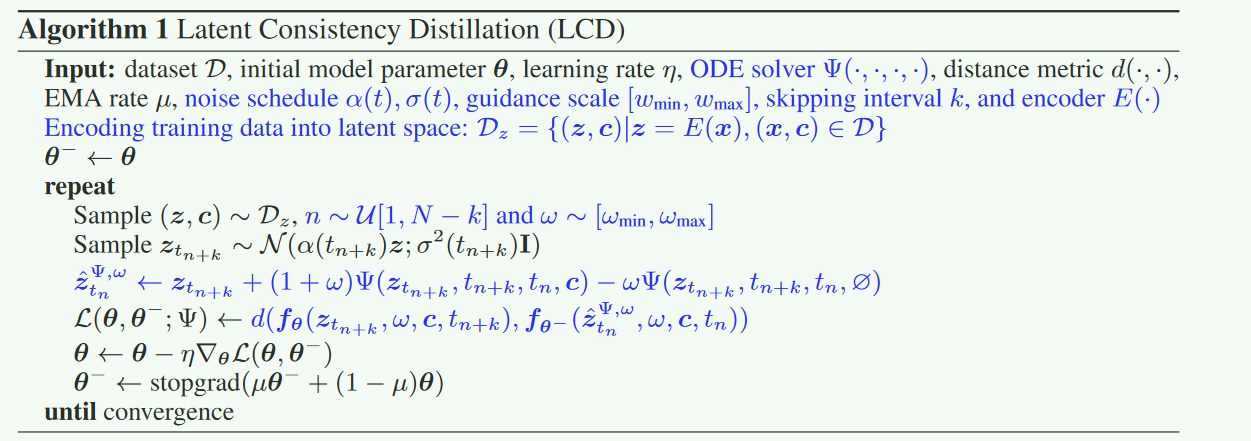
\includegraphics[width=\linewidth]{image/LCD.jpg}
\caption{Latent Consistency Distillation}
\label{fig:LCD}
\end{figure}

\subsection{从端点一致性到轨迹映射与平均速度}
前面的自一致性条件本身还不够：如果网络总输出同一个常数，成对输出也会相等。
因此需要端点边界，例如 $f(x,0)=x$；
参数化中的 $c_{\rm skip}(0)=1,c_{\rm out}(0)=0$ 就用于落实这件事。
实际训练往往在一个小的正噪声 $\varepsilon$ 处设置边界，避免直接求零噪声分数。
此外，时间对的选取、离散化与距离函数都影响训练，
iCT 改进了独立一致性训练的这些设计，并区分了它与教师蒸馏时目标网络更新的作用。
不能把“两个输出相等”单独当作完整训练方案。\cite{cm,ict}

LCM 仍主要学习到固定低噪声端点的映射。
如果将目标时刻也作为输入，写成 $G(x,t,s)$，便可学习从 $t$ 到任意较低时刻 $s$ 的轨迹映射。
理想流映射满足
\[
G(x,t,t)=x,\qquad
G(G(x,t,r),r,s)=G(x,t,s),\quad s\leq r\leq t.
\]
第二式说的是，沿同一速度场先走一段再走一段，与直接走到目标时刻相同。
CTM 沿这个方向学习概率流轨迹，并配合相应训练约束。
这是把端点一致性扩展到两时刻之间的映射，并不是角色身份的一致性。\cite{ctm}

MeanFlow 则从平均速度继续推导。为了与前文扩散记号一致，
这里仍令 $t$ 向噪声端增加，生成时从 $t$ 走向 $s<t$。
对速度场 $v$ 的真实轨迹，定义
\[
u(x_t,s,t)=\frac1{t-s}\int_s^t v(x_r,r)\,\mathrm dr,
\qquad x_s=x_t-(t-s)u(x_t,s,t).
\]
这不是仅在起点求值的瞬时速度，而是整段轨迹的平均。
固定 $s$，沿轨迹对两边 $(t-s)u=\int_s^t v\,\mathrm dr$ 求导：
\[
u+(t-s)(\partial_tu+D_xu\,v)=v,
\]
从而得到
\[
u=v-(t-s)(\partial_tu+D_xu\,v).
\]
右边的方向导数可以用 Jacobian--vector product 计算，无需显式保存完整 Jacobian。
训练还需规定条件速度标签、停止梯度和权重等细节；
这个恒等式说明的是两时刻平均速度与瞬时速度的关系，
不是说把任意已训练的瞬时速度模型做一次大 Euler 步就能精确生成。\cite{meanflow,theorybook}



\subsection{角色一致性}

这里的“角色一致性”指跨图像、跨镜头保持同一身份或外观，
与前面一致性模型的“同一 ODE 轨迹映射到相同端点”是两个不同的问题。
参考图特征、身份编码、微调与注意力条件可以提供身份约束，
但仅使用 LCM 等少步模型本身不会自动保证角色身份稳定。


\section{离散状态的扩散}
前面的空间分数使用 $\nabla_x$，要求连续坐标上的可微密度。
但这不意味着离散数据一定要先经 VAE 才能做扩散。
对于词表、类别等有限状态，可以直接规定随机替换或遮蔽的马尔可夫过程，
再学习相应的逆转移。这里用概率比值代替空间梯度。

先看一个小时间步。设从状态 $i$ 跳到 $j$ 的速率为 $Q_t(i,j)$，$i\ne j$，
并令 $Q_t(i,i)=-\sum_{j\ne i}Q_t(i,j)$。
若 $p_t$ 写为行向量，主方程就是 $\partial_tp_t=p_tQ_t$。
对逆向时钟，贝叶斯公式给出从当前 $j$ 跳回 $i$ 的速率
\[
\bar Q_t(j,i)=Q_t(i,j)\frac{p_t(i)}{p_t(j)},\qquad p_t(j)>0.
\]
推导只需将
$P(X_{t-h}=i\mid X_t=j)$ 写为正向转移概率乘以前一时刻边缘、再除以当前边缘，
对 $i\ne j$ 除以 $h$ 并取极限。
SEDD 学习的离散分数正是这样的密度比值，而不是对 token 编号求导。\cite{sedd}

掩码扩散是更具体的例子。假设一个 token 到时间 $t$ 仍保留的概率为 $\rho_t$，
否则变成吸收态 $\mathtt{MASK}$。对 $s<t$ 且 $\rho_s>\rho_t$，
在已知 $X_t=\mathtt{MASK}$ 时，逆向重新显露原 token 的概率为
\[
P(X_s\ne\mathtt{MASK}\mid X_t=\mathtt{MASK})
=\frac{\rho_s-\rho_t}{1-\rho_t}.
\]
分子是“在 $s$ 尚未遮蔽、到 $t$ 已被遮蔽”的概率，分母是当前已遮蔽概率。
至于显露成哪个 token，则由模型在上下文与时间条件下预测，
相应训练常写成带时间权重的遮蔽位置交叉熵。
多位置迭代可以并行更新，但同一步的条件独立预测、有限步采样和具体重遮蔽策略仍会影响结果。
它与自回归逐 token 分解、连续高斯去噪有联系，也各有自己的逆过程定义。\cite{mdlm,theorybook}




\section{应用}

以下保留原稿记录的训练设置与应用观察，作为阅读当时工作的笔记。
它们属于不同模型和任务，不宜直接横向比较，也不代表当前项目统一的训练预算。
具体部署与设计、短视频、短剧的简要交付流程放在完整书稿后续章节。


\begin{itemize}
    \item 1千万文本对数据，模型参数22M ：DeepSpeed ZeRO-2 +  8 V100 + 1M steps + bs=8 per GPU
    \item 5千万图文对+1千万高质量人数据：48 NVIDIA H800 GPUs (80GB) + 2 per GPU ( InstantID)
    \item 3百万图文对数据，模型参数1431.6M(367M)： 10 epochs using 8 Tesla A100 GPUs+progressive 
    \item 百万数据+万ID+caption：8 A100 GPUs + two weeks + bs=48
    \item 256-coreTPU-v3 pod, training DiT-L takes 12 hours.
    \item 通常是128*60=48*180：沉没成本比较大
    \item 组合思路难度小，混杂的库太多，数据集制作繁杂，比较占资源(意义不大)
    \item 优点：1d 扩散，simplify unet, only one bvh(400+frames) data, any topology,  4GGPU memory, 1 hour training cost, 5 infer applications，long frames generator
\end{itemize}

\subsection{多模态}

排列组合+卡+数据，太多了。

\subsubsection{VAE、CLIP、U-Net、U-ViT、DiT等模块}

前面的公式规定了“学习什么”，这里再接上“由什么模块来学”。
像素空间模型直接对图像张量加噪；潜空间模型先用编码器得到 $z=\mathcal E(x)$，
再对 $z$ 加噪、训练去噪网络，最后由 $\mathcal D$ 解码。
这样能减少空间计算量，也把生成质量的上限部分交给了编解码器。
潜变量模型的似然不能不经解码器分析就当成像素数据的似然。

U-Net 用不同分辨率的卷积特征和跳跃连接预测噪声、分数或其它标签；
U-ViT、DiT 等则把图像或潜变量转成 token，用 Transformer 建模。
预测标签由训练目标决定，换成 Transformer 并不自动改变 DDPM 或 Flow Matching 的概率原理。
时间条件告诉网络当前噪声级，CLIP 等文本编码器把提示词转成条件特征。
下式给出交叉注意力的基本运算：图像特征提供查询，文本特征提供键和值。
这里将 token 排成矩阵的行，投影矩阵乘在特征右侧，
使 $Q\in\mathbb R^{N\times d}$、$K,V\in\mathbb R^{M\times d}$，
因此 $QK^\top$ 给出每个图像位置对各文本位置的注意力权重。


\begin{equation}
  \begin{aligned} & 
    \text { Attention }(\mathbf{Q}, \mathbf{K}, \mathbf{V})=\operatorname{softmax}\left(\frac{\mathbf{Q K}^{\top}}{\sqrt{d}}\right) \cdot \mathbf{V} \\ 
    & \text { where } \mathbf Q=\varphi_i(\mathbf z_i)\mathbf W_Q^{(i)},\quad\mathbf K=\tau_\theta(y)\mathbf W_K^{(i)},\quad\mathbf V=\tau_\theta(y)\mathbf W_V^{(i)} \\ 
    & \text { and } \mathbf W_Q^{(i)}\in\mathbb R^{d_c^i\times d},\quad\mathbf W_K^{(i)},\mathbf W_V^{(i)}\in\mathbb R^{d_r\times d}, \varphi_i\left(\mathbf{z}_i\right) \in \mathbb{R}^{N \times d_c^i}, \tau_\theta(y) \in \mathbb{R}^{M \times d_r}
  \end{aligned}
\end{equation}


\subsection{Rectified Flow}

前面从加噪 SDE 推出概率流 ODE，是先规定随机过程，再导出确定性速度。
现在换一个起点：直接规定数据与噪声之间的插值，再学习能搬运这组边缘分布的速度。
这里保留 $t=0$ 为数据、$t=1$ 为噪声的约定。
取 $X_0\sim p_{\rm data}$ 与 $Z\sim\mathcal N(0,I)$ 独立，令
\[
X_t=(1-t)X_0+tZ,\qquad \dot X_t=Z-X_0.
\]
训练时两端点都已知，因此可以直接回归
\[
\mathcal L_{\rm CFM}(\theta)=
 \mathbb E_{t,X_0,Z}\|v_\theta(X_t,t)-(Z-X_0)\|^2.
\]
但生成时并不知道当前点对应哪一对 $X_0,Z$，所以模型实际学到的是条件平均
\[
v^*(x,t)=\mathbb E[Z-X_0\mid X_t=x].
\]
为什么这个条件平均仍能生成所需分布？对任意光滑测试函数 $\varphi$，
先对插值求导，再使用条件期望：
\begin{align}
\frac{\mathrm d}{\mathrm dt}\mathbb E[\varphi(X_t)]
 &=\mathbb E[\nabla\varphi(X_t)^\top(Z-X_0)]\\
 &=\int p_t(x)\nabla\varphi(x)^\top v^*(x,t)\,\mathrm dx.
\end{align}
分部积分后得到 $\partial_tp_t=-\nabla\cdot(p_tv^*)$。
因此在适当存在唯一性与边界条件下，这个速度场的 ODE 具有插值指定的逐时边缘分布。
训练时无需先数值求解 ODE 来获得监督；采样时则从噪声端反向积分。
这就是条件 Flow Matching 将困难的边缘速度回归改成已知条件标签回归的原因。
\cite{fm,rf,flow-guide}

这里的“直线”首先是每对训练端点之间的条件插值。
经过同一个 $x$ 的端点对可能很多，条件平均后的速度会随空间与时间改变，
所以由它积分出来的轨迹未必都是直线，更不保证一个 Euler 步就到达真实数据。
例如上面模型在 $t=1$ 处有 $X_1=Z$，且
$v^*(z,1)=z-\mathbb E[X_0]$。若直接从1走到0做一个 Euler 大步，
得到的是 $z-v^*(z,1)=\mathbb E[X_0]$，所有样本都坍缩为数据均值。
这与从整个时间区间积分得到正确端点分布并不矛盾。

Rectified Flow 的 reflow 再用已有流把噪声与生成端点配成新对，
在新配对上重新进行直线回归，希望减少轨迹弯曲与少步误差。
它改变的是端点耦合；独立配对、模型产生的配对与最优传输配对不是同一个东西。
二次代价最优传输寻找使 $\mathbb E\|Z-X_0\|^2$ 最小的合法耦合，
而一个小批量内的最优匹配只近似这个全分布问题。
Schrödinger Bridge 又保留了随机参考过程，在端点约束下最小化路径 KL；
它与确定性运输有联系，也不能仅凭“连接两端分布”就与 Rectified Flow 等同。
这些区别决定了训练配对、路径随机性与实际采样的含义。\cite{theorybook}


\subsubsection{条件控制}

无条件模型描述 $p_t(x)$，给定文本、类别或其它观测 $c$ 时，希望描述 $p_t(x\mid c)$。
若已有噪声条件分类器，贝叶斯公式对 $x$ 求导给出
\[
\nabla_x\log p_t(x\mid c)=\nabla_x\log p_t(x)+\nabla_x\log p_t(c\mid x).
\]
右边分类器要接收相应噪声级的 $x_t$，不能直接拿只识别干净图像的分类器代替。
这就是 classifier guidance 的分数分解。

CFG 则在训练时随机丢弃条件，让同一个网络能够预测有条件与无条件分数，采样时组合为
\[
s_{\rm cfg}=s_{\rm uncond}+w(s_{\rm cond}-s_{\rm uncond}).
\]
这里 $w=1$ 是通常的条件分数；前面 LCM 使用的
$(1+\omega)s_{\rm cond}-\omega s_{\rm uncond}$ 对应 $w=1+\omega$。
高斯路径下噪声预测与分数相差同一个时间尺度，所以也可以组合噪声预测。
对固定 $t$，理想分数的这个线性组合形式上对应
\[
\nabla_x\log\bigl[p_t(x\mid c)^w p_t(x)^{1-w}\bigr].
\]
但这些逐时倾斜密度未必共同构成原扩散的边缘路径，
不能据此无条件声称最终生成分布恰好是同样幂次的端点密度乘积。
增大引导也可能放大预测误差，损失多样性或造成数值不稳定。

对逆问题也是如此。例如观测满足 $y=Ax_0+\eta$，
反向过程需要的似然是
$p_t(y\mid x_t)=\int p(y\mid x_0)p(x_0\mid x_t)\,\mathrm dx_0$。
用去噪均值 $\hat x_0(x_t)$ 代入 $p(y\mid\hat x_0)$ 是一种近似，
它省略了整个干净后验的不确定性。外加控制网络、参考特征或奖励偏好也会改变条件建模或训练目标，
需要分别说明监督来自哪里，不能仅用“加了条件”推出精确后验采样的结论。
\cite{theorybook}


\subsection{变大}
\subsubsection{SDXL}

分辨率与模型规模提高后，同一套噪声回归仍要处理更多空间位置和更复杂条件。
SDXL 等潜空间模型增加去噪网络与条件编码能力，配合分辨率、裁剪等附加条件。
这里变化的是表示和模型容量；前向路径、预测标签及采样调度仍应逐一核对，
不能只由模型名称判断它采用哪一个损失或求解器。


\subsection{Finetune}
\subsubsection{LORA}

微调继续在目标数据上优化原有去噪或速度回归目标。
LoRA 将某个线性层的更新限制为 $\Delta W=BA$，其中
$W\in\mathbb R^{m\times n}$、$B\in\mathbb R^{m\times r}$、
$A\in\mathbb R^{r\times n}$，通常 $r\ll\min(m,n)$。
这样训练的参数从 $mn$ 降为 $r(m+n)$，原权重可以冻结。
它限制的是参数更新空间，并不单独构成新的生成概率模型；
低秩、少量数据与条件过拟合之间的取舍仍取决于具体任务。


\subsection{3D重建}

生成式先验可作为多视图重建或三维表示优化的约束，但单张图像存在深度、遮挡和视角歧义。
二维去噪得分较高，并不自动说明多个视角来自同一个三维场景。
因此需要区分图像生成先验、相机与几何约束、三维表示和最终渲染监督各自的作用。


\subsection{动画动作生成}
\subsubsection{SinMDM}

动作数据可以是关节位置、旋转或其它时序表示；扩散过程先作用于选定的数值表示。
SinMDM 一类单片段运动扩散工作利用短序列内部重复结构学习新的动作变化，
其任务设置与大规模文本条件动作生成不同。
生成后仍需检查骨长、足部接触与时间连续性；逐元素回归损失本身不会自动落实这些运动学条件。



\section{框架实现}
\subsection{Diffusers、SCEPTER}

这类框架把模型、训练组件与采样调度组织成可复用实现。
阅读代码时，可以沿“加噪器—预测标签—损失权重—采样器”检查它与前面公式的对应，
尤其注意训练时的时间编号和推理时跳步的时间网格是否一致。


\subsection{ComfyUI、WebUI、Fooocus}

这类界面将编码、条件、去噪、解码及后处理连接成工作流。
相同界面可以承载不同模型与求解器，所以复现时应记录实际权重、节点、调度、随机种子和条件设置。
服务部署的吞吐、显存与延迟问题在后面的部署章节简述。








% Detailed theory extensions follow the retained manuscript without replacing it.
\chapter{潜变量、能量模型与连续概率流}
\label{supp:objectives}

前面已经沿 DDPM、NCSN 和 Score SDE 的顺序，把扩散模型的主要推导写了一遍。
但这里还有几个问题没有展开：VAE 的编码器和解码器到底在共同优化什么？
能量模型为什么需要负样本？既然 ODE 可以算似然，为什么还要使用分数匹配与流匹配？
这些问题分别对应参考书第2、3、5章及附录C中的内容。下面从原来已经用过的公式继续推导，
不再重新写一遍 DDPM 的配方过程。\cite{theorybook}

\section{从联合分布看 VAE 的训练}
\subsection{重建项和潜变量正则项是怎么分出来的}
设生成联合分布为 $p_\theta(x,z)=p(z)p_\theta(x\mid z)$，
编码器为 $q_\phi(z\mid x)$。前面已经有
\[
\mathcal L_{\rm ELBO}(x)=\mathbb E_{q_\phi(z\mid x)}
 \log\frac{p_\theta(x,z)}{q_\phi(z\mid x)}.
\]
把联合分布拆开，而不是直接把这个式子叫作一个损失，就能看出两部分各自的作用：
\begin{align}
\mathcal L_{\rm ELBO}(x)
 &=\mathbb E_q[\log p_\theta(x\mid z)+\log p(z)-\log q_\phi(z\mid x)]\\
 &=\mathbb E_q\log p_\theta(x\mid z)
   -D_{\rm KL}(q_\phi(z\mid x)\|p(z)).
\label{supp:vae-decomposition}
\end{align}
第一项要求从编码结果恢复观测；第二项约束编码分布与生成时使用的先验之间的差异。
只把训练样本编码后重建得很好，还不能推出从先验随机抽一个 $z$ 就能解码得很好。
原因是训练时的 $z$ 来自 $q_\phi(z\mid x)$，生成时却来自 $p(z)$，这两个来源需要接起来。

例如使用对角高斯编码器和固定方差高斯解码器：
\[
q_\phi(z\mid x)=\mathcal N(\mu_\phi(x),\operatorname{diag}\sigma_\phi^2(x)),
\quad p_\theta(x\mid z)=\mathcal N(D_\theta(z),\tau^2I).
\]
取负对数，去掉与参数无关的常数，重建部分变成
\[
-\mathbb E_q\log p_\theta(x\mid z)
=\frac1{2\tau^2}\mathbb E_q\|x-D_\theta(z)\|^2+\text{const}.
\]
若先验为标准高斯，KL 项进一步成为
\[
D_{\rm KL}(q_\phi\|p)
=\frac12\sum_j\left(\mu_{\phi,j}^2+\sigma_{\phi,j}^2
 -1-\log\sigma_{\phi,j}^2\right).
\]
于是得到常见的“重建误差加 KL”。它不是两个经验损失的任意拼接，
而是相应概率假设下负 ELBO 的展开。
若把 KL 的系数另设为 $\beta\ne1$，或者加入感知、对抗损失，
则需要说明已经改变了这一原始目标，不能把修改后的全部目标仍当作同一个似然下界。

\subsection{两个误差：生成模型误差与推断误差}
定义数据与编码器组成的联合分布
$q_\phi(x,z)=p_{\rm data}(x)q_\phi(z\mid x)$。直接展开联合 KL：
\begin{align}
D_{\rm KL}(q_\phi(x,z)\|p_\theta(x,z))
 &=\mathbb E_{q_\phi}\log
 \frac{p_{\rm data}(x)q_\phi(z\mid x)}{p_\theta(x)p_\theta(z\mid x)}\\
 &=D_{\rm KL}(p_{\rm data}\|p_\theta)
 +\mathbb E_{p_{\rm data}}D_{\rm KL}(q_\phi(z\mid x)\|p_\theta(z\mid x)).
\end{align}
这里第二项是近似后验与模型后验之间的误差，非负，所以联合 KL 控制了数据边缘的 KL。
固定生成模型而只优化编码器时，确实是在缩小推断误差；
同时优化两者时，模型后验也在变化，不能仅凭 ELBO 增大就说这两项都分别单调下降。

还有一个容易忽略的点：即使编码网络足够深，输出仍若限定为单个对角高斯，
它也不能表示任意多峰后验。增加网络层数改变了均值和方差如何依赖 $x$，
没有把“单个高斯”的分布族限制消掉。使用层级潜变量、可逆变换或更复杂的后验族，
处理的就是这个问题。把潜变量展开成 $x_1,\ldots,x_T$ 并固定前向加噪，
又回到了前文 DDPM 的多层变分模型。

\section{能量模型的极大似然与负相}
前面已经写过 $p_\theta(x)=\exp[-E_\theta(x)]/Z_\theta$。
对数据负对数似然求参数梯度，先不要把 $Z_\theta$ 丢掉：
\begin{align}
\nabla_\theta[-\log p_\theta(x)]
 &=\nabla_\theta E_\theta(x)+\nabla_\theta\log Z_\theta,\\
\nabla_\theta\log Z_\theta
 &=\frac{\int-\nabla_\theta E_\theta(y)e^{-E_\theta(y)}\,\mathrm dy}{Z_\theta}
 =-\mathbb E_{p_\theta(y)}\nabla_\theta E_\theta(y).
\end{align}
所以平均损失的梯度为
\[
\nabla_\theta\mathcal J
=\mathbb E_{p_{\rm data}}\nabla_\theta E_\theta(X)
 -\mathbb E_{p_\theta}\nabla_\theta E_\theta(Y).
\label{supp:ebm-gradient}
\]
梯度下降降低真实数据的能量，同时相对提高模型当前产生的样本的能量。
后一项称为负相，需要来自当前模型的样本，因此训练内部又嵌入了采样问题。
使用短链 Langevin 代替平衡分布，会引入近似；不能把少走几步的负样本当作精确极大似然。

而空间分数 $\nabla_x\log p_\theta=-\nabla_xE_\theta$ 不含 $Z_\theta$，
所以 NCSN 的分数回归绕开了直接计算负相。这里有个边界：
一个任意向量网络未必是某个全局标量能量的梯度。
在光滑、单连通区域，梯度场的 Jacobian 应当对称；普通分数网络的参数化并未强制这一点。
即便如此，它仍能作为反向 SDE 或 ODE 的系数使用，只是不能因此声称已经显式构造出一个归一化 EBM。

若两个严格正密度在连通区域具有相同空间分数，则
$\nabla\log(p/q)=0$，故 $p=Cq$，再由归一化得到 $C=1$。
如果支撑集分成互不连通的几块，每一块却可以有不同的常数，
局部分数本身不能决定各块之间的质量比例。
高斯扰动让分布在整个空间为正，也就缓解了原稿提到的支撑与低密度连接问题。

\section{Normalizing Flow：从映射恢复密度}
\subsection{为什么要有 Jacobian 行列式}
设 $Z\sim\pi$，$X=F_\theta(Z)$，$F_\theta:\mathbb R^d\to\mathbb R^d$
可逆且 Jacobian 非奇异。局部体积满足
$\mathrm dx=|\det D_zF_\theta|\mathrm dz$。
同一小块的概率质量不变，因此
\begin{align}
p_\theta(x)\,\mathrm dx&=\pi(z)\,\mathrm dz,\\
\log p_\theta(F_\theta(z))
 &=\log\pi(z)-\log|\det D_zF_\theta(z)|.
\end{align}
例如 $x=az+b$，一维密度会除以 $|a|$。拉长区间的同时降低密度，
才能保持总概率不变。它与前面的 VAE 不同：这里的编码是生成映射的精确逆，
不用另设近似后验，但需要同维、可逆以及可计算的行列式。

若 $F=F_K\circ\cdots\circ F_1$，则
\[
\log p(x_K)=\log\pi(x_0)
 -\sum_{k=1}^K\log|\det D F_k(x_{k-1})|.
\]
这解释了常见可逆网络为什么设计三角 Jacobian 或耦合层。
例如 $y_1=x_1$，$y_2=x_2\odot e^{a(x_1)}+b(x_1)$，
其行列式为 $\exp[\sum_j a_j(x_1)]$，不必计算完整高维行列式。

\subsection{连续极限、散度与 Hutchinson 迹估计}
将一步映射改成 $x_{t+h}=x_t+h v_\theta(x_t,t)$，
利用 $\log\det(I+hA)=h\operatorname{tr}A+O(h^2)$，得到
\[
\frac{\mathrm d}{\mathrm dt}\log p_t(x_t)
=-\operatorname{tr}D_xv_\theta(x_t,t).
\]
这就是前文 ODE 似然公式的来源。若 $v$ 对空间局部 Lipschitz、轨迹在区间内不爆炸，
其流具有相应的唯一性与反向求解性质。ODE 的可逆性不要求每个有限步 Euler 映射都自动可逆；
离散数值方法还有自己的步长条件。

高维时，显式构造 $D_xv$ 很贵。取独立随机向量 $\xi$，满足
$\mathbb E[\xi\xi^\top]=I$，则
\begin{align}
\mathbb E_\xi[\xi^\top D_xv\,\xi]
 &=\mathbb E_\xi\operatorname{tr}(D_xv\,\xi\xi^\top)
 =\operatorname{tr}D_xv.
\end{align}
于是通过向量与 Jacobian 的乘积估计散度，而不是存储 $d\times d$ 矩阵。
一次噪声向量给出的是随机估计，实际还叠加数值积分误差。
因此“连续流有精确的密度变换公式”和“实现返回毫无误差的似然数值”需要分开。
似然训练还须对 ODE 积分结果反向求导；后面的流匹配则用条件回归避免在训练循环里求解整条 ODE。

\section{一般扩散矩阵与反向过程}
原稿主要使用 $g(t)I$，这让分数前的系数很简洁。
若扩散还依赖状态，设
\[
\mathrm dX_t=f(X_t,t)\mathrm dt+G(X_t,t)\mathrm dW_t,
\quad A(x,t)=G(x,t)G(x,t)^\top.
\]
在密度和系数足够光滑的情形，前向方程为
\[
\partial_tp=-\sum_i\partial_i(f_ip)
 +\frac12\sum_{i,j}\partial_i\partial_j(A_{ij}p).
\]
定义 $(\nabla\cdot A)_i=\sum_j\partial_j A_{ij}$，则概率流速度可取
\[
v=f-\frac12\nabla\cdot A-\frac12A\nabla\log p.
\label{supp:general-pf}
\]
因为 $\sum_j\partial_j(A_{ij}p)=p(\nabla\cdot A)_i+(A\nabla p)_i$，
把它代入 $-\nabla\cdot(pv)$，恰好恢复前向方程。

用正向增加的反时钟 $r=T-t$，令 $Y_r=X_{T-r}$。
相应逆扩散在适当时间反转条件下的漂移为
\[
\bar f(x,r)=-f(x,T-r)+(\nabla\cdot A)(x,T-r)
 +A(x,T-r)\nabla\log p_{T-r}(x).
\]
扩散协方差仍为 $A(x,T-r)$。
当 $A=g(t)^2I$ 时，空间散度消失，就退回原稿公式。
因此状态依赖扩散的逆过程不能只把 $g^2$ 换成一个矩阵而漏掉散度项。
同时，仅验证边缘方程还不充分证明完整路径时间反转；反向漂移的结论需要时间反转定理的条件。

\section{Girsanov：分数误差界从哪里来}
设两个过程使用相同、可逆的扩散矩阵 $G$，漂移分别为 $b$ 和 $\tilde b$。
先假定初始分布相同，记 $u=G^{-1}(b-\tilde b)$。
在相应绝对连续与指数可积条件下，以 $\tilde P$ 为参考路径测度，
Girsanov 的密度比可写为
\[
\log\frac{\mathrm dP}{\mathrm d\tilde P}
=\int_0^T u_t^\top\mathrm dW_t^{\tilde P}
 -\frac12\int_0^T\|u_t\|^2\mathrm dt.
\]
在 $P$ 下，$\mathrm dW^{\tilde P}=\mathrm dW^P+u\mathrm dt$，
所以再对 $P$ 取期望，零均值随机积分消失，得到
\[
D_{\rm KL}(P\|\tilde P)
=\frac12\mathbb E_P\int_0^T
 \|G^{-1}(b-\tilde b)\|^2\mathrm dt.
\]
若初始分布不同，路径 KL 的链式分解再加上初始 KL。
将两个过程都写到增加的反时钟，精确逆漂移与模型逆漂移之差为
$g(t)^2(\nabla\log p_t-s_\theta)$，再除以扩散尺度 $g(t)$，
就得到原稿出现的 $g(t)^2$ 加权分数平方误差。
\begin{align}
D_{\rm KL}(P^{\rm rev}\|P_\theta)
 &=D_{\rm KL}(p_T\|\pi)
 +\frac12\int_0^Tg(t)^2\mathbb E_{p_t}
  \|s_\theta-\nabla\log p_t\|^2\mathrm dt.
\label{supp:path-kl}
\end{align}
再取生成端点这一边缘，KL 不增加，所以得到数据端的上界。
这说明权重为什么不是任意的，也说明为什么这里不能直接比较 ODE 与 SDE 的路径 KL：
确定性轨迹和非退化随机轨迹的路径测度通常不满足这套绝对连续条件。
在零噪声附近，还需检查积分是否有限；若在 $\varepsilon>0$ 终止，
上式先控制的是 $p_\varepsilon$，不是省略最后一步后的精确原始数据分布。\cite{theorybook,sde}

\chapter{流匹配的构造、条件技巧与训练等价}
\label{supp:flow}

原稿 Rectified Flow 小节已经写了直线插值和条件平均，这里继续处理一般情况。
问题是：只要人为画出一条从数据到噪声的分布路径，就一定知道怎样训练吗？
同一个路径对应的速度是不是唯一的？噪声预测、分数预测和速度预测又在什么意义下等价？
这几件事在参考书第5、6章中是分开推导的，不能只用一个“等价”统称。\cite{theorybook,fm,flow-guide}

\section{条件回归的共同基础}
\subsection{先证明一个平方损失的分解}
设 $X$ 是网络输入，$Y$ 是可以采到、但对同一个输入未必唯一的监督标签。
记 $m(X)=\mathbb E[Y\mid X]$，对任意可测预测函数 $h$，有
\begin{align}
\|h(X)-Y\|^2
 &=\|h(X)-m(X)\|^2+\|Y-m(X)\|^2\\
 &\quad-2(h(X)-m(X))^\top(Y-m(X)).
\end{align}
条件于 $X$ 时，最后一项的期望为零，因为
$\mathbb E[Y-m(X)\mid X]=0$。故
\[
\mathbb E\|h(X)-Y\|^2
=\mathbb E\|h(X)-m(X)\|^2
 +\mathbb E\|Y-m(X)\|^2.
\label{supp:regression-projection}
\]
第二项与网络无关，所以用随机标签回归，和用不可直接计算的条件平均回归，
有相同的总体最优解；目标值却相差一个常数。
即使网络已经达到这个最优解，原始训练损失也可能不为零，
剩下的是同一输入对应多种标签所带来的条件方差。

将 $X$ 换成 $(X_t,t)$，这个结论同时适用于 DSM、噪声预测、干净样本预测与 CFM。
它要求的是标签的条件平均正确，不要求每个训练标签都等于生成时应该使用的确定速度。
有限数据、有限网络容量和实际优化当然还会带来额外误差。

\subsection{条件分数与条件速度为什么分别成立}
设条件变量为 $C$，条件密度是 $p_t(x\mid c)$，且
$p_t(x)=\int p_t(x\mid c)\,q(\mathrm dc)$。
在能够交换积分与微分、且 $p_t(x)>0$ 时，
\begin{align}
\nabla\log p_t(x)
 &=\frac{\int\nabla p_t(x\mid c)q(\mathrm dc)}{p_t(x)}\\
 &=\mathbb E[\nabla\log p_t(X_t\mid C)\mid X_t=x].
\end{align}
这是分数的条件技巧。对速度，要从每个条件路径自己的连续性方程开始：
\[
\partial_tp_t(x\mid c)=-\nabla\cdot[p_t(x\mid c)u_t(x\mid c)].
\]
对 $c$ 积分，得到
\begin{align}
\partial_tp_t(x)
 &=-\nabla\cdot\int p_t(x\mid c)u_t(x\mid c)q(\mathrm dc)\\
 &=-\nabla\cdot[p_t(x)v_t(x)],\quad
v_t(x)=\mathbb E[u_t(X_t\mid C)\mid X_t=x].
\label{supp:conditional-velocity}
\end{align}
再用式\eqref{supp:regression-projection}，就可以训练可计算的条件速度，而不必计算边缘速度。
前一个恒等式来自密度求导，后一个来自概率通量相加；这就是二者形式类似的原因。

\section{一般高斯路径的条件速度}
设 $X_0\sim p_{\rm data}$、$Z\sim\mathcal N(0,I)$ 独立，定义
\[
X_t=a_tX_0+b_tZ,\quad t\in[0,1],\quad
a_0=1,b_0=0,a_1=0,b_1=1.
\]
这里沿用原稿“0为数据、1为噪声”的方向，生成时反向积分。
条件于 $X_0=x_0$，这是一个均值 $a_tx_0$、标准差 $b_t$ 的高斯路径。
若在 $0<t<1$ 上 $b_t>0$，则相应条件速度为
\begin{align}
u_t(x\mid x_0)
 &=\dot a_tx_0+\dot b_t\frac{x-a_tx_0}{b_t}\\
 &=\frac{\dot b_t}{b_t}x+
 \left(\dot a_t-\frac{\dot b_ta_t}{b_t}\right)x_0.
\label{supp:affine-conditional}
\end{align}
因为沿同一个条件轨迹，高斯坐标 $Z$ 不变，对插值直接求导即可。
也可以固定两端 $(X_0,Z)$，使用标签 $\dot a_tX_0+\dot b_tZ$。
二者的条件平均产生相同边缘速度，但每条条件路径耦合的含义不同。

结合高斯条件分数
$s_t(x\mid x_0)=-(x-a_tx_0)/b_t^2$，可解出
\[
\mathbb E[X_0\mid X_t=x]
=\frac{x+b_t^2s_t(x)}{a_t}.
\]
将它代回条件速度的平均，得到
\[
v_t(x)=\frac{\dot a_t}{a_t}x+
 \left(\frac{\dot a_t}{a_t}b_t^2-b_t\dot b_t\right)s_t(x).
\label{supp:affine-marginal}
\]
端点处可能出现 $a_t$ 或 $b_t$ 为零，所以这些除法形式先在内部时间成立，
端点需要用极限或另一种不奇异的参数化处理。
直线路径取 $a_t=1-t,b_t=t$，就回到了原稿的 $Z-X_0$ 标签。

\subsection{路径、耦合和真实 ODE 轨迹是三个对象}
两端边缘并不规定联合分布。独立采样、按条件标签配对、最优传输配对，
都可能具有相同的两端边缘，却给出不同的中间分布。
给定一种端点耦合 $\gamma(x_0,z)$，再给定插值函数 $I_t(x_0,z)$，
才确定了训练用的随机路径及其边缘。
最后对条件速度取平均得到的 ODE 轨迹，又未必就是原先每一对端点的插值线。
多条条件路径在同一个时空点相遇时，网络只能输出它们的平均速度。
因此“用直线训练”本身不能保证“ODE 轨迹逐条都是直线”。

\section{一个能完全算完的 Flow Matching 例子}
为看清条件平均的影响，取一维独立高斯
$X_0\sim\mathcal N(0,\sigma_0^2)$、$Z\sim\mathcal N(0,\sigma_1^2)$。
令 $X_t=(1-t)X_0+tZ$，则
\[
c_t=\operatorname{Var}(X_t)=(1-t)^2\sigma_0^2+t^2\sigma_1^2.
\]
高斯条件均值给出
\begin{align}
v_t(x)&=\mathbb E[Z-X_0\mid X_t=x]\\
 &=\frac{t\sigma_1^2-(1-t)\sigma_0^2}{c_t}x
 =\frac{\dot c_t}{2c_t}x.
\end{align}
ODE 因此可以直接积分：
\[
\frac{\mathrm dx_t}{x_t}=\frac12\mathrm d\log c_t,
\qquad x_t=\sqrt{\frac{c_t}{c_s}}x_s.
\]
若从 $t=1$ 的噪声反向积分到0，就得到方差 $\sigma_0^2$ 的数据分布。
但是每一对独立训练端点之间的直线一般不服从这个比例关系。
训练配对与生成配对不同，边缘分布却能一致，这正是条件技巧的用途。

\section{相同边缘为什么不唯一确定速度}
已知 $p_t$，若 $v_t$ 满足连续性方程，再取满足
$\nabla\cdot(p_tw_t)=0$ 的场，则 $v_t+w_t$ 产生同一个密度演化。
例如二维标准高斯不随时间变化，$v=0$ 可以保持它；
取反对称矩阵
$K=\left(\begin{smallmatrix}0&-\omega\\\omega&0\end{smallmatrix}\right)$，
$w(x)=Kx$ 也可以保持它。因为
\[
\nabla\cdot(pKx)=\nabla p^\top Kx+p\operatorname{tr}K
=-p\,x^\top Kx+0=0.
\]
前一组粒子原地不动，后一组持续旋转；每一时刻的总体分布相同，端点映射却不同。
所以“训练正确边缘速度”还包含我们选择哪一种条件路径和哪一个速度代表的问题。
最优传输接下来会在这些可能性中再加入代价准则。

\section{信噪比、时间重参数与目标权重}
\subsection{似然权重与对数信噪比}
若高斯路径来自线性 SDE
$\mathrm dX=f(t)X\mathrm dt+g(t)\mathrm dW$，则
\[
\dot a=fa,\qquad \frac{\mathrm d}{\mathrm dt}b^2=2fb^2+g^2.
\]
定义对数信噪比 $\ell_t=\log(a_t^2/b_t^2)$，直接求导：
\[
\dot\ell_t=2\dot a_t/a_t-\frac{2b_t\dot b_t}{b_t^2}
=-\frac{g(t)^2}{b_t^2}.
\]
又因分数与噪声预测差一个 $-1/b_t$，路径 KL 的误差项变为
\begin{align}
\frac12\int g(t)^2\mathbb E\|s_\theta-s_t\|^2\mathrm dt
 &=\frac12\int[-\dot\ell_t]
 \mathbb E\|\epsilon_\theta-\hat\epsilon_t\|^2\mathrm dt.
\end{align}
如果 $\ell$ 单调，这就是在对数信噪比坐标上的噪声预测误差积分。
均匀采样 $t$ 并使用无权噪声 MSE，通常与这个权重不同。
原稿中“简化损失是一种重新加权”，在这里就有了连续时间的具体表达。

\subsection{换时钟与重新分配训练资源}
设 $t=\psi(r)$，$\psi$ 单调增加。若只是给同一条 ODE 换时钟，则
\[
\frac{\mathrm dx}{\mathrm dr}=\psi'(r)v(x,\psi(r)).
\]
速度必须乘上 $\psi'$。对前向 SDE，扩散尺度还要乘 $\sqrt{\psi'}$，
因为布朗增量的方差与时间增量成正比。
但若只改变训练抽样的时间密度 $q(t)$，却保持样本路径和标签不变，
改变的是训练资源分配。要无偏估计原来 $\int w(t)L_t\mathrm dt$，应使用
\[
\mathbb E_{t\sim q}\left[\frac{w(t)}{q(t)}L_t\right],\qquad q(t)>0
\ \text{在目标权重非零处成立}.
\]
不补这个权重，就变成另一个目标。它可能训练得更好，但不是同一个积分的无偏估计。

\section{给同一条概率路径加入随机性}
前面概率流从 SDE 走到 ODE；也可以反过来。
设 $v_t$ 已经使 $p_t$ 满足连续性方程，取只依赖时间的 $\eta(t)\geq0$，定义
\[
\mathrm dX_t=\left[v_t(X_t)+\frac{\eta(t)^2}{2}s_t(X_t)\right]\mathrm dt
 +\eta(t)\mathrm dW_t.
\label{supp:same-marginal-family}
\]
代入 Fokker--Planck，额外两项为
$-\tfrac12\eta^2\nabla\cdot(p_ts_t)+\tfrac12\eta^2\Delta p_t=0$。
因此在精确分数、匹配初始分布和适当正则性下，它仍具有相同的 $p_t$。
反向增加时钟下的漂移则是 $-v_t+\tfrac12\eta^2s_t$。

这给出一个共同边缘下的 ODE/SDE 采样族，但它们的路径联合分布不同。
模型分数、速度都只有近似值时，前面的抵消也只有近似意义；
不能保证随意增加随机性就一定改善样本质量。
同理，标签换算、相同总体最优解、相同边缘、相同端点配对、相同路径分布，
分别是不同层次的关系；每次说“等价”之前都需要说明正在比较哪一层。\cite{theorybook}

\section{给定扰动核，怎样恢复一个前向 SDE}
前面从线性 SDE 算出了 $a_t,b_t$，现在反过来。
假设只规定条件核 $p_t(x\mid x_0)=\mathcal N(a_tx_0,b_t^2I)$，
想找 $\mathrm dX=f(t)X\mathrm dt+g(t)\mathrm dW$ 实现这组核。
由条件均值和方差的演化方程可解出
\[
f(t)=\frac{\dot a_t}{a_t},\qquad
g(t)^2=2b_t\dot b_t-2\frac{\dot a_t}{a_t}b_t^2
=-b_t^2\dot\ell_t.
\]
因此内部时间上必须有 $g(t)^2\geq0$，即信噪比沿前向时间不增加。
不是任意两条光滑系数曲线都能在这个方向上构成实值线性 Itô 扩散。
恢复出来的过程给这些边缘核增加了一种 Markov 路径耦合；
训练时各时刻独立采噪声，并不表示整条训练随机路径已经按这条 SDE 耦合。

例如 VE 取 $a_t=1$、$b_t^2=\sigma(t)^2$，则
$f=0$、$g^2=\mathrm d\sigma^2/\mathrm dt$。
VP 的 $a_t^2+b_t^2=1$ 则给出 $g^2=-2\dot a_t/a_t$，
对应原稿 $f=-\beta/2$、$g^2=\beta$。

再取直线路径 $a_t=1-t,b_t=t$，内部时间给出
\[
f(t)=-\frac1{1-t},\qquad g(t)^2=\frac{2t}{1-t}.
\]
条件方差的确满足
$\frac{\mathrm d}{\mathrm dt}t^2=2f(t)t^2+g(t)^2=2t$。
但系数在 $t\to1$ 时发散，说明相同的仿射边缘路径在确定性插值表述中很简单，
在这一线性 SDE 表述中却可能有奇异端点。
实际需要在内部区间讨论，或另选时间尺度、终端近似与采样方式。
这也解释了为什么代数上能换算，不表示所有表述在数值上同样方便。

\chapter{最优传输、Schrödinger 桥与分布梯度流}
\label{supp:transport}

前面已经知道同一组分布可以由不同的速度连接。现在继续问：如果还要求运输代价最小，
应该选择哪一个映射或哪一条路径？这就进入最优传输问题。
如果再保留随机扩散，并要求尽量少地改变一个参考过程，就进入 Schrödinger 桥问题。
这部分对应参考书第7章及附录B，补上原稿此前仅提到名字的内容。\cite{theorybook}

\section{Monge、Kantorovich 与两端耦合}
为直接讨论从源到目标的运输，本章用 $r\in[0,1]$ 表示运输时间，
$\mu$ 表示源分布，$\nu$ 表示目标分布。它们可以取噪声和数据，也可以是任意两组分布。
给定代价 $c(x,y)$，Monge 问题寻找确定映射 $T$：
\[
\inf_{T:\,T_\#\mu=\nu}\int c(x,T(x))\,\mu(\mathrm dx).
\]
$T_\#\mu=\nu$ 表示先从 $\mu$ 抽样再作用 $T$，得到的分布恰好为 $\nu$。
这个要求与“某几个样本看起来靠近目标”不同，它约束的是完整边缘分布。

确定映射不能在同一个源点处分拆质量。如果源只有一个原子、目标有两个不同原子，
这类映射甚至不存在。因此放宽为联合分布 $\gamma$，只要求两端边缘分别为 $\mu,\nu$：
\[
\inf_{\gamma\in\Pi(\mu,\nu)}\int c(x,y)\,\gamma(\mathrm dx,\mathrm dy).
\]
这就是 Kantorovich 问题。$\gamma$ 可以将一处质量拆给多个目标。
当代价为 $\|x-y\|^2$、两端二阶矩有限时，最优值定义为 $W_2^2(\mu,\nu)$。
在源分布绝对连续等条件下，二次代价最优耦合可由凸函数的梯度映射实现，
即 Brenier 映射；离散、奇异分布则不能直接套用这组结论。

一维时可以看得更直观。若累积分布函数连续且严格增加，令
$T(x)=F_\nu^{-1}(F_\mu(x))$，就把相同分位数对应起来。
对 $x_1<x_2$、$y_1<y_2$，交叉配对与顺序配对的代价差为
\[
(x_1-y_2)^2+(x_2-y_1)^2
 -(x_1-y_1)^2-(x_2-y_2)^2
=2(x_2-x_1)(y_2-y_1)\geq0.
\]
所以二次代价不鼓励交叉配对。对高斯
$\mu=\mathcal N(m_0,\sigma_0^2)$、$\nu=\mathcal N(m_1,\sigma_1^2)$，结果为
\[
T(x)=m_1+\frac{\sigma_1}{\sigma_0}(x-m_0),\qquad
W_2^2=(m_1-m_0)^2+(\sigma_1-\sigma_0)^2.
\]
这是一条可以算完的最优映射，不能据此推断任意扩散流都自动学到它。

\section{从端点代价走向动态动能}
\subsection{Benamou--Brenier 表述}
对绝对连续的粒子轨迹 $X_r$，
\[
\|X_1-X_0\|^2=\left\|\int_0^1\dot X_r\,\mathrm dr\right\|^2
\leq\int_0^1\|\dot X_r\|^2\mathrm dr.
\]
同一对端点之间，匀速直线使这个不等式取等。
如果整个总体由速度 $v_r$ 推动，密度为 $p_r$，则需要满足
\[
\partial_rp_r+\nabla\cdot(p_rv_r)=0,\qquad p_0=\mu,\quad p_1=\nu.
\]
在相应有限二阶矩条件下，动态最优传输写为
\[
W_2^2(\mu,\nu)=\inf_{p,v}
 \int_0^1\int\|v_r(x)\|^2p_r(x)\,\mathrm dx\mathrm dr.
\label{supp:bb}
\]
任一合法速度场的动能都是这个最优值的上界。
反过来，从最优端点耦合的直线插值构造动态路径，可达到相应最优值，
这说明静态与动态表述的联系；一般结论涉及弱解与测度路径的技术条件。

引入动量 $m=pv$ 后，目标变成 $\int\|m\|^2/p$，约束变成
$\partial_rp+\nabla\cdot m=0$，凸性因而更清楚。
若对带 $1/2$ 的动能目标引入乘子 $\varphi$，分部积分后的内部项是
\[
\int p\left(\frac12\|v\|^2-\partial_r\varphi-v^\top\nabla\varphi\right).
\]
先对 $v$ 取驻点得到 $v=\nabla\varphi$；在光滑正密度区域再得到
\[
\partial_r\varphi+\frac12\|\nabla\varphi\|^2=0.
\]
这就是 Hamilton--Jacobi 方程。最优速度要同时满足质量守恒与最优性条件，
普通 Flow Matching 只拟合指定路径的速度，没有自动加入全部这些约束。

\subsection{为什么保持正确分布还不等于最优运输}
取二维标准高斯作为源和目标。恒等映射的代价为0，所以已经最优。
若让所有粒子旋转一个非零角度，目标仍是标准高斯，但
\[
\mathbb E\|RX-X\|^2=2d-2\operatorname{tr}R>0
\]
（$R\ne I$ 的二维旋转，$d=2$）。这给出一个最直接的反例：
正确边缘和可逆确定性流并不充分保证最优传输。
概率流 ODE 还受它原先指定的加噪路径约束，因此也不能仅由分数精确就推出端点映射最优。
即使每个时刻的速度是某个标量势的梯度，跨时间组合的最终映射也不自动是凸势的梯度。

\section{Rectification 与 reflow 能保证什么}
现在把前章的条件速度放进动态代价。
设一组端点 $A,B$ 来自任意耦合，条件插值为 $X_r=(1-r)A+rB$，
条件速度为 $B-A$，边缘速度为 $v_r(x)=\mathbb E[B-A\mid X_r=x]$。
条件 Jensen 不等式给出
\[
\mathbb E\|v_r(X_r)\|^2\leq\mathbb E\|B-A\|^2.
\]
设 $Y_r$ 是这个边缘场的 ODE 轨迹，并具有相同逐时边缘，则
\begin{align}
\mathbb E\|Y_1-Y_0\|^2
 &\leq\int_0^1\mathbb E\|v_r(Y_r)\|^2\mathrm dr\\
 &=\int_0^1\mathbb E\|v_r(X_r)\|^2\mathrm dr
 \leq\mathbb E\|B-A\|^2.
\label{supp:reflow-bound}
\end{align}
所以把旧配对换成 ODE 产生的新配对，可以得到二次端点代价不增加的理想结论。
下一轮再对这些新端点做直线回归，就是 reflow 的基本过程。

但上面的两个不等式只保证“不比旧耦合更贵”，没有说已经达到所有耦合中的全局最小值。
它还假设速度准确、ODE 正确求解、边缘确实匹配。
实际网络误差和有限步积分会破坏精确结论。少步生成质量与运输代价也不是同一个评价量。

\section{熵正则传输与 Sinkhorn 缩放}
离散样本上，设两端概率向量为 $\mu_i,\nu_j$，代价为 $C_{ij}$。
熵正则问题可写为
\[
\min_{\gamma\geq0}\sum_{i,j}C_{ij}\gamma_{ij}
 +\varepsilon\sum_{i,j}\gamma_{ij}\log\frac{\gamma_{ij}}{\mu_i\nu_j},
\quad \gamma\mathbf1=\mu,\quad\gamma^\top\mathbf1=\nu.
\]
对内部正解引入边缘约束的乘子，求 $\gamma_{ij}$ 的驻点，得到
$\gamma_{ij}=a_iK_{ij}b_j$，其中 $K_{ij}=\exp(-C_{ij}/\varepsilon)$，
与两端质量有关的因子可吸收到 $a,b$。
边缘约束于是转化为逐元素缩放：
\[
a\leftarrow\mu/(Kb),\qquad b\leftarrow\nu/(K^\top a).
\]
这就是 Sinkhorn 迭代的基本形式。小 $\varepsilon$ 更重视运输代价，
较大 $\varepsilon$ 更重视相对独立耦合的熵正则。
当 $\varepsilon\to0$ 时，在适当紧性和可积条件下可讨论最优值与最优计划的极限，
不能简单将可能具有无限 KL 的确定性最优耦合代入一个有限熵上界证明。
实际还需要数值稳定的对数域计算。

小批量上计算一次 Sinkhorn，只解决该批经验分布之间的问题。
它可以为 CFM 提供更好的训练配对，但与全数据分布的最优耦合仍有采样差异。

\section{Schrödinger 桥：约束的是整条随机路径}
\subsection{路径 KL 的静态分解}
设参考路径分布为 $R$，其端点联合分布为 $R_{01}$。
桥问题要求 $P_0=\mu,P_1=\nu$，同时最小化 $D_{\rm KL}(P\|R)$。
将路径按两个端点条件化，KL 链式分解给出
\begin{align}
D_{\rm KL}(P\|R)
 &=D_{\rm KL}(P_{01}\|R_{01})\\
 &\quad+\mathbb E_{(A,B)\sim P_{01}}
 D_{\rm KL}(P(\cdot\mid A,B)\|R(\cdot\mid A,B)).
\end{align}
固定端点耦合后，第二项的最小值为0，由参考过程的条件桥实现。
因此问题分为两步：先找最优端点耦合，再在给定端点下使用参考桥。

若参考为 $\mathrm dX_r=\sqrt\varepsilon\mathrm dW_r$、$R_0=\mu$，
转移密度与 $\exp[-\|b-a\|^2/(2\varepsilon)]$ 成比例，故对固定两端边缘，
\[
D_{\rm KL}(\gamma\|R_{01})
=\frac1{2\varepsilon}\mathbb E_\gamma\|B-A\|^2
 +D_{\rm KL}(\gamma\|\mu\otimes\nu)+\text{const}.
\]
这说明桥问题与熵正则运输的联系，也给出了系数的来源。
条件于端点 $A=a,B=b$，内部时间的 Brownian bridge 为
\[
X_r\mid a,b\sim\mathcal N((1-r)a+rb,\varepsilon r(1-r)I).
\]
条件均值是直线，但路径还有随机波动。
仅从独立端点采这组桥，通常不等于已经求出了最优桥，因为最优端点耦合那一步还没有完成。

\subsection{控制能量、势函数与交替投影}
令参考 SDE 为 $\mathrm dX=f\mathrm dr+g\mathrm dW$，
受控漂移改成 $f+u$，扩散保持相同。
由前章 Girsanov 公式，
\[
D_{\rm KL}(P\|R)=D_{\rm KL}(\mu\|R_0)
 +\frac12\mathbb E_P\int_0^1\frac{\|u(X_r,r)\|^2}{g(r)^2}\,\mathrm dr.
\]
所以桥问题是在两端约束下最小化对参考过程的控制能量。
解的路径密度在适当条件下具有
$\mathrm dP^*/\mathrm dR=a(X_0)b(X_1)$ 的形式。
终端势的条件平均
$h(x,r)=\mathbb E_R[b(X_1)\mid X_r=x]$
满足参考生成算子的后向方程，额外前向漂移为 $g^2\nabla\log h$。
初始因子 $a$ 则与另一个势共同落实两端边缘。

从算法角度，一次只匹配终端边缘的 KL 投影为
\[
\frac{\mathrm dP^{\rm new}}{\mathrm dP^{\rm old}}
=\frac{\nu(X_1)}{p_1^{\rm old}(X_1)}.
\]
下一次再按 $\mu(X_0)/p_0^{\rm new}(X_0)$ 修正初始边缘，交替进行，
就是路径空间 IPF 的基本想法。一次投影会改变另一端，因此往往需要迭代。

普通扩散模型固定前向过程，由数据端自然产生一个终端分布，
这个分布通常只近似预设高斯。对这个自然端点，原参考过程可以是零控制的特殊桥；
但若两端分布被另外指定且不兼容，就需要非零控制，不能把普通反向扩散直接叫作任意端点的最优桥。

\section{Wasserstein 梯度流与 Langevin 的关系}
前面优化的是连接两端的运输代价；现在改为让一个分布逐渐降低某个泛函。
用 $\tau$ 表示这种分布演化时间，以免与模型的噪声时间混淆。
取 $\mathcal F(p)=D_{\rm KL}(p\|\pi)$，其一阶变分为
$\delta\mathcal F/\delta p=\log(p/\pi)+1$。
选择下降速度
\[
w_\tau=-\nabla\frac{\delta\mathcal F}{\delta p}
=\nabla\log\pi-\nabla\log p_\tau.
\]
代回连续性方程，得到
\[
\partial_\tau p=\Delta p-\nabla\cdot(p\nabla\log\pi),
\]
恰好是 $\mathrm dX=\nabla\log\pi\mathrm d\tau+\sqrt2\mathrm dW$ 的 Fokker--Planck 方程。
在边界项消失时还可以验证
\[
\frac{\mathrm d}{\mathrm d\tau}\mathcal F(p_\tau)
=-\int p_\tau\left\|\nabla\frac{\delta\mathcal F}{\delta p}\right\|^2\mathrm dx\leq0.
\]
这把“分数指向高密度”和“整体分布的 KL 下降”连接起来。
但神经网络参数的梯度下降被限制在一个参数族中，未必等于这里自由的分布空间梯度流。

最后补一个熵与 Fisher 信息的关系。若 $\partial_\tau p=\tfrac12\Delta p$，
微分熵 $h(p)=-\int p\log p$ 满足
\begin{align}
\frac{\mathrm dh}{\mathrm d\tau}
 &=-\frac12\int(\Delta p)\log p
 =\frac12\int\frac{\|\nabla p\|^2}{p}
 =\frac12\mathbb E_p\|\nabla\log p\|^2.
\end{align}
第一步用了总质量导数为0，第二步用了分部积分。
因此高斯平滑使熵增加，其变化率由空间分数的平方决定。
它也是前文熵、分数和扩散这三个对象之间一条具体的数学联系。

\chapter{条件生成、逆问题与偏好对齐}
\label{supp:guidance}

原稿中 CFG 的公式已经列出，但仍有一串问题需要接着回答：
为什么加的是似然的梯度？分类器应该接收哪个噪声级？
把引导系数调大之后，得到的分布究竟是什么？
如果条件来自一个测量方程或一个偏好评分，又应该怎样进入生成过程？
本章按参考书第8章展开这些问题。\cite{theorybook}

\section{条件分布的分数与分类器引导}
设条件 $c$ 在前向加噪时不变，$p_t(x\mid c)$ 是带噪条件分布。
贝叶斯公式给出
\[
p_t(x\mid c)=\frac{p_t(c\mid x)p_t(x)}{p(c)},\qquad
\nabla_x\log p_t(x\mid c)=s_t(x)+\nabla_x\log p_t(c\mid x).
\]
分母只依赖 $c$，所以对 $x$ 求导后消失。
将右边代入原稿的反向 SDE，就得到 classifier guidance。
若使用原先递减的扩散时钟，新增漂移为
$-g(t)^2\nabla_x\log p_t(c\mid x)$，
但乘上负的 $\mathrm dt$ 后，实际采样会朝分类器认为更符合条件的方向移动。
若改用递增反时钟，这个控制项直接写成正号。

这里不能忽略下标 $t$。训练分类器时，应先从有标签数据中取 $(x_0,c)$，
再按同一个前向核构造 $x_t$，优化
\[
\mathbb E_{t,x_0,c,x_t}[-\log C_\psi(c\mid x_t,t)].
\]
只有这样，分类器才近似在估计采样时需要的噪声条件似然。
仅在干净样本上准确的分类器，并不因此在高噪声输入上给出正确梯度。
即便分数和分类器都精确，起始端也应匹配 $p_T(x\mid c)$；
当噪声足够大而条件信息已被抹去时，才常用同一个高斯先验来近似各个条件的终端。

\section{CFG 的训练、尺度约定与跨时间兼容性}
\subsection{为什么同一个网络能做有条件与无条件预测}
训练时以概率 $\rho$ 将 $c$ 替换为空条件 $\varnothing$，记处理后的条件为 $\tilde c$。
例如噪声回归目标为
\[
\mathbb E\|\epsilon_\theta(a_tx_0+b_t\epsilon,t,\tilde c)-\epsilon\|^2.
\]
空条件分支的数据并未只来自某个类别，所以它学习无条件噪声预测；
保留条件的分支学习条件预测。总体最优解在两种输入下分别是相应的条件平均。
采样时组合
\[
\epsilon_{\rm cfg}=\epsilon_u+w(\epsilon_c-\epsilon_u),\qquad
s_{\rm cfg}=s_u+w(s_c-s_u).
\]
这里 $w=0$ 为无条件，$w=1$ 为通常的条件预测。
如果代码使用 $(1+\omega)\epsilon_c-\omega\epsilon_u$，则 $w=1+\omega$。
讨论强度前先对照这个定义，否则同一个“scale=1”可能对应不同含义。

\subsection{固定时间的幂次密度不等于完整采样的端点定律}
在分数精确的理想情形，固定 $t$ 时
\[
s_{\rm cfg}=\nabla\log[p_t(x)p_t(c\mid x)^w].
\]
这只说明当时的向量场是一个倾斜密度的分数。
要使不同 $t$ 的倾斜密度成为同一条前向扩散的边缘，还必须满足 Fokker--Planck 方程。
把这个要求直接展开，可以看到缺少的条件。

令 $u_t(x)$ 为任意倾斜势，定义
$\tilde p_t=p_te^{u_t}/Z_t$，前向算子为
$L_t^*p=-\nabla\cdot(fp)+\tfrac12g^2\Delta p$。
由于 $p_t$ 本身满足前向方程，乘积求导与空间乘积展开给出
\begin{align}
\frac{\partial_t\tilde p_t-L_t^*\tilde p_t}{\tilde p_t}
 &=\partial_tu_t+f^\top\nabla u_t-g^2s_t^\top\nabla u_t\\
 &\quad-\frac{g^2}{2}(\Delta u_t+\|\nabla u_t\|^2)
 -\partial_t\log Z_t.
\label{supp:tilt-residual}
\end{align}
右边必须为零，才有跨时间兼容性。
精确分类条件对应 $u_t=\log p_t(c\mid x)$，$w=1$ 时确实恢复真实条件路径；
但任意损失、任意时间调度、任意幂次一般没有这个保证。
因此增大 CFG 可以改变条件服从性和样本外观，却不能未经检查就说终点精确服从
$p_0(x\mid c)^w p_0(x)^{1-w}$。
这类误差在求解器无限精确时仍可能存在，和数值误差不是同一个来源。

\section{逆问题：为什么需要带噪似然}
设观测为 $y=\mathcal A(x_0)+\eta$，$\eta\sim\mathcal N(0,\sigma_y^2I)$。
生成目标是 $p(x_0\mid y)$，在噪声时间 $t$ 需要
\[
p_t(y\mid x_t)=\int p(y\mid x_0)p(x_0\mid x_t)\,\mathrm dx_0.
\label{supp:noisy-likelihood}
\]
这里积分的是一个分布，而不是单个去噪结果。
若只知道去噪均值 $m_t(x_t)=\mathbb E[X_0\mid x_t]$，
把积分近似为 $p(y\mid m_t(x_t))$，就得到常见的均值代入思路。
其引导梯度是
\[
\nabla_{x_t}\log p(y\mid m_t(x_t))
=\frac1{\sigma_y^2}J_{m_t}(x_t)^\top
 J_{\mathcal A}(m_t)^\top[y-\mathcal A(m_t)].
\]
梯度必须经过去噪器和观测算子一起传播。
把 $m_t$ 停止梯度会改变这个公式；保留或近似哪些 Jacobian，需要单独说明。

\subsection{用高斯例子看被忽略的后验方差}
若 $X_0\mid x_t\sim\mathcal N(m_t,C_t)$，$\mathcal A(x)=Ax$，则积分可精确完成：
\[
Y\mid x_t\sim\mathcal N(Am_t,\Sigma_t),\qquad
\Sigma_t=\sigma_y^2I+AC_tA^\top.
\]
当 $C_t$ 不依赖 $x_t$ 时，精确引导为
\[
\nabla_{x_t}\log p_t(y\mid x_t)
=J_{m_t}^\top A^\top\Sigma_t^{-1}(y-Am_t).
\]
均值代入会把 $\Sigma_t$ 换成 $\sigma_y^2I$，因此忽略高噪声下的干净后验不确定性，
可能过度相信测量残差。
若后验协方差也随输入变化，精确求导还会出现协方差和行列式的导数，
不能直接沿用上式。这也说明相关近似何时比较可信：后验足够集中，或者不确定性相对测量噪声很小。

\subsection{二阶 Tweedie 关系}
原稿的一阶 Tweedie 公式给出均值。对 $X_t=a_tX_0+b_tZ$，再求一次导数，
可把协方差也写出来。后验对输入的对数导数为
\[
\nabla_x\log p(x_0\mid x)
=\frac{a_t}{b_t^2}[x_0-m_t(x)].
\]
因此，对均值的每个坐标求导可得
\[
J_{m_t}(x)=\frac{a_t}{b_t^2}\operatorname{Cov}(X_0\mid X_t=x).
\]
再由 $m_t=(x+b_t^2s_t(x))/a_t$ 得到
\[
\operatorname{Cov}(X_0\mid X_t=x)
=\frac{b_t^2}{a_t^2}\left[I+b_t^2\nabla_x^2\log p_t(x)\right].
\label{supp:second-tweedie}
\]
它在适当可微、矩存在及内部时间条件下成立。
这给高阶分数和后验不确定性一个明确联系，
但网络近似的 Hessian 未必使右边保持半正定，实际使用仍需检查数值与模型误差。

\section{终端奖励与 Doob 的 $h$ 变换}
有时条件不是测量方程，而是最终样本的奖励 $R(x)$。
这里改用生成时间 $r$，从噪声 $r=0$ 走到数据 $r=1$，参考过程为
$\mathrm dX=b\mathrm dr+g\mathrm dW$。
定义
\[
h(x,r)=\mathbb E\left[\exp(R(X_1)/\kappa)\mid X_r=x\right],\qquad\kappa>0.
\]
由 Markov 性和后向方程，
\[
\partial_rh+b^\top\nabla h+\frac{g^2}{2}\Delta h=0,
\qquad h(x,1)=e^{R(x)/\kappa}.
\]
以终端因子重加权整条参考路径后，新的局部漂移为
\[
b^h=b+g^2\nabla\log h.
\]
为什么不能直接用 $\nabla R(x_r)$ 代替它？因为 $h$ 评价的是
“从当前状态继续生成，最终可能获得的指数奖励平均”，并非当前带噪样本的奖励。

还要处理起始分布。若整条路径按 $e^{R(X_1)/\kappa}/Z$ 重加权，
其初始边缘也变成 $\rho_0(x)h(x,0)/Z$，终端才是精确指数倾斜。
若坚持保持原来的初始边缘，则条件路径需除以各自的 $h(X_0,0)$，
最后得到的端点不再自动等于同一个全局倾斜公式。
在高噪声起点几乎不含终端信息时，$h(x,0)$ 近似常数，这种区别才可能很小。
这也是无训练奖励引导需要近似未来价值或校正权重的原因。

\section{分数蒸馏：把图像先验传给另一个生成器}
如果优化变量是三维场景、可微渲染器或另一个生成器的参数，
输出图像写为 $x_0=g_\theta(z)$，可以希望它的加噪分布接近扩散先验。
考虑一个理想平滑目标
\[
\mathcal J(\theta)=\mathbb E_{t,z}
 D_{\rm KL}\bigl(\mathcal N(a_tg_\theta(z),b_t^2I)\|p_t(\cdot\mid c)\bigr).
\]
单个高斯的熵与均值无关，所以使用重参数化后，梯度为
\begin{align}
\nabla_\theta\mathcal J
 &=-\mathbb E_{t,z,\epsilon}
 a_tJ_{g_\theta}^\top s_t(x_t\mid c)\\
 &=\mathbb E_{t,z,\epsilon}\frac{a_t}{b_t}
 J_{g_\theta}^\top[\hat\epsilon_t(x_t,c)-\epsilon].
\end{align}
第二行减去的 $\epsilon$ 对 $z$ 条件下期望为零，可作为控制变量。
这解释了 SDS 类更新中“预测噪声减实际噪声”的来源。
实践还会改变时间权重、使用 CFG 或其它梯度近似，因此需要说明具体目标。

更关键的是，这里平均的是每个 $z$ 的单个加噪高斯相对先验的 KL，
并非生成器整体混合分布的同一个 KL。
若 $q_t$ 表示混合边缘，则有
\[
\mathbb E_zD_{\rm KL}(q_t(\cdot\mid z)\|p_t)
=D_{\rm KL}(q_t\|p_t)+I(Z;X_t).
\]
多出的互信息项会改变优化行为。
因此把 SDS 视为对任意生成器分布的无偏完整分布匹配，需要额外论证。

\section{KL 正则奖励优化与 DPO}
\subsection{先求分布空间中的最优解}
固定条件 $c$，设参考模型为 $\pi_{\rm ref}(x\mid c)$，奖励为 $r(c,x)$。
考虑
\[
\max_\pi\left\{\mathbb E_\pi r-\beta D_{\rm KL}(\pi\|\pi_{\rm ref})\right\},\quad\beta>0.
\]
对密度作变分并加入归一化约束，得到
\[
r-\beta[\log(\pi/\pi_{\rm ref})+1]+\lambda=0.
\]
因此在归一化常数有限时，
\[
\pi^*(x\mid c)=\frac{\pi_{\rm ref}(x\mid c)e^{r(c,x)/\beta}}{Z(c)}.
\label{supp:reward-optimum}
\]
也可将目标改写为 $\beta\log Z-\beta D_{\rm KL}(\pi\|\pi^*)$，直接验证最优性。
这是所有密度上的理想最优解；有限神经网络和实际训练不一定能达到它。

\subsection{成对偏好怎样变成对数概率比}
采用 Bradley--Terry 偏好模型
$P(x_w\succ x_l\mid c)=\operatorname{sigmoid}(r(c,x_w)-r(c,x_l))$。
由式\eqref{supp:reward-optimum}，奖励差可写为
\[
r_w-r_l=\beta\left[
 \log\frac{\pi^*(x_w\mid c)}{\pi_{\rm ref}(x_w\mid c)}
 -\log\frac{\pi^*(x_l\mid c)}{\pi_{\rm ref}(x_l\mid c)}\right].
\]
条件归一化常数在同条件的差里消失，遂得到 DPO 形式的目标
\[
-\mathbb E\log\operatorname{sigmoid}\left(\beta\left[
 \log\frac{\pi_\theta(x_w\mid c)}{\pi_{\rm ref}(x_w\mid c)}
 -\log\frac{\pi_\theta(x_l\mid c)}{\pi_{\rm ref}(x_l\mid c)}\right]\right).
\]
它以成对比较的分类损失拟合隐式奖励差，不要求先单独拟合一个显式奖励网络。
但偏好模型、数据分布和参考约束仍是实际假设。

\subsection{为什么扩散 DPO 不能直接用噪声 MSE 冒充样本似然}
离散扩散的端点似然要积分掉整条潜轨迹，直接计算通常困难。
若比较路径分布，相同先验下可以分解
\[
\log\frac{P_\theta(x_{0:T}\mid c)}{P_{\rm ref}(x_{0:T}\mid c)}
=\sum_{t=1}^T\log
 \frac{p_\theta(x_{t-1}\mid x_t,c)}{p_{\rm ref}(x_{t-1}\mid x_t,c)}.
\]
共享固定高斯方差时，每个对数转移比可转成均值误差差，再转成带系数的噪声误差差。
这使训练能抽样时间与加噪监督，但路径 KL、端点 KL、变分代理并非同一个对象。
尤其 $\log\operatorname{sigmoid}$ 是非线性的，把期望放到其内外会改变目标。
所以实际 Diffusion-DPO 推导需要说明使用哪一种路径或变分代理、怎样取期望与共享噪声，
而不是直接把一个无权 MSE 差写成精确的端点对数似然比。\cite{theorybook}

\chapter{数值求解与可学习的快速生成}
\label{supp:fast}

原稿已给出 DDIM 和 DPM 系列的一阶积分关系，也介绍了一致性与蒸馏。
本章继续补上参考书第9--11章中尚未展开的部分：误差阶数、DEIS、多阶构造、
时间并行、两步合一步的训练标签，以及一般流映射与平均速度如何训练。
\cite{theorybook}

\section{数值阶数、稳定性与生成质量}
\subsection{局部误差为什么会累积成全局误差}
暂用增加的生成时间 $r$，考虑 $\dot x=v(x,r)$。
Euler 一步为 $x_{n+1}=x_n+h v(x_n,r_n)$。
对精确解作 Taylor 展开，
\[
x(r+h)=x(r)+hv(x,r)+\frac{h^2}{2}
 [\partial_rv+D_xv\,v]+O(h^3).
\]
所以从一个精确起点出发，一步局部截断误差为 $O(h^2)$。
若速度对空间是 $L$-Lipschitz，则累积误差满足
\[
e_{n+1}\leq(1+Lh)e_n+Ch^2.
\]
对固定总时间求和，得到 $e_N=O(h)$，这就是 Euler 一阶的含义。
Heun 先预测 $\tilde x=x_n+hv(x_n,r_n)$，再用
\[
x_{n+1}=x_n+\frac h2[v(x_n,r_n)+v(\tilde x,r_n+h)]
\]
修正，在相应光滑和稳定条件下为全局二阶。
单步需要两次网络求值，所以比较速度时还要记录 NFE，而不是只数步数。

阶数结论比较的是同一向量场的数值解与精确解。
若向量场本身已有学习误差，更多步、更高阶只会更接近这个学习到的 ODE，
不自动意味着更接近真实数据。强 CFG 还可能增大局部变化与刚性，使稳定性比形式阶数更先成为限制。

\subsection{SDE 的强误差与弱误差}
Euler--Maruyama 对 $\mathrm dX=b\mathrm dr+g\mathrm dW$ 的一步是
$X_{n+1}=X_n+hb(X_n,r_n)+g(X_n,r_n)\sqrt hZ_n$。
强误差比较使用同一布朗驱动的逐样本距离，弱误差比较
$|\mathbb E\varphi(X_N)-\mathbb E\varphi(X(r_N))|$。
对一般乘性噪声、满足相应光滑与增长条件的情形，常见结论是强阶 $1/2$、弱阶1；
特殊加性噪声问题可有更好的性质，不能把一个阶数套到所有设置。

以稳定 OU 过程 $\mathrm dX=-\kappa X\mathrm dr+\sigma\mathrm dW$ 为例，
精确一步噪声方差为 $\sigma^2(1-e^{-2\kappa h})/(2\kappa)$，
Euler 一步噪声方差却是 $\sigma^2h$。
它的离散稳定方差由 $V=(1-\kappa h)^2V+\sigma^2h$ 给出：
\[
V_{\rm EM}=\frac{\sigma^2}{2\kappa-\kappa^2h},\qquad 0<\kappa h<2.
\]
有限步长下与真实 $\sigma^2/(2\kappa)$ 不同。
这说明即使分数完全准确，离散采样仍可以引入分布偏差。

\section{DEIS：历史预测怎样进入积分}
沿用原稿 $a_t,b_t$ 和半对数信噪比 $\lambda=\log(a_t/b_t)$，
从高噪声 $t$ 到较低噪声 $s$ 的积分式为
\[
x_s=\frac{a_s}{a_t}x_t-a_s\int_{\lambda_t}^{\lambda_s}
 e^{-\lambda}\epsilon_\theta(x_\lambda,\lambda)\,\mathrm d\lambda.
\]
DDIM 将积分里的网络输出当常数。DEIS 类方法则存下已经完成的时刻预测
$(\lambda_j,E_j)$，构造 Lagrange 多项式
\[
P_k(\lambda)=\sum_{j=0}^k L_j(\lambda)E_j,
\qquad L_j(\lambda)=\prod_{m\ne j}\frac{\lambda-\lambda_m}{\lambda_j-\lambda_m}.
\]
在历史点上它是插值，向下一步区间使用时则是外推。
代回积分，更新变成
\[
x_s\approx\frac{a_s}{a_t}x_t-a_s\sum_{j=0}^k B_jE_j,
\qquad B_j=\int_{\lambda_t}^{\lambda_s}e^{-\lambda}L_j(\lambda)\,\mathrm d\lambda.
\]
系数只由调度和历史节点决定，可以预先计算；本步不用为每个历史锚点重新调用网络。
在原始时间或其它坐标里也能构造相应的加权外推，
这里用 $\lambda$ 说明共同的指数积分思想，不把不同坐标的系数混用。

例如两点时，$P_1=E_n+(\lambda-\lambda_n)(E_n-E_{n-1})/(\lambda_n-\lambda_{n-1})$。
它使用历史斜率估计下一段的变化。
但第一步没有两点历史，需要先用低阶启动；之后逐渐提高阶数。
锚点来自数值轨迹，本身含误差，所以插值多项式的精确性不等于真实网络轨迹的精确性。

\section{DPM-Solver 二阶项的具体来历}
记 $h=\lambda_s-\lambda_t>0$，
$E(\lambda)=\epsilon_\theta(x_\lambda,\lambda)$，沿轨迹展开
$E(\lambda_t+u)=E_t+uE_t'+O(u^2)$。
两个需要的积分分别为
\[
\int_0^he^{-u}\mathrm du=1-e^{-h},\qquad
\int_0^hue^{-u}\mathrm du=1-(1+h)e^{-h}.
\]
利用 $a_se^{-\lambda_t}=b_se^h$，得到
\[
x_s=\frac{a_s}{a_t}x_t-b_s(e^h-1)E_t
 -b_s(e^h-h-1)E_t'+O(h^3).
\]
导数是沿轨迹的总导数，不是只对网络时间输入求偏导。
可以选择内部点 $\lambda_m=\lambda_t+qh$，$0<q\leq1$，
先做一阶预测
\[
x_m=\frac{a_m}{a_t}x_t-b_m(e^{qh}-1)E_t,
\qquad E_t'\approx\frac{\epsilon_\theta(x_m,m)-E_t}{qh}.
\]
代回便得到一个二阶单步指数积分构造。
它需要当前点与内部点两次网络求值；多步版本则改为用历史差商。
$e^h-h-1$ 在 $h$ 很小时为 $h^2/2+O(h^3)$，实现宜用稳定的指数差或级数处理消减误差。
\cite{dpm}

DPM-Solver++ 对数据预测 $D(\lambda)$ 作展开，积分权重改为 $e^\lambda$。
同样计算可得
\[
x_s=\frac{b_s}{b_t}x_t+a_s(1-e^{-h})D_t
 +a_s(h-1+e^{-h})D_t'+O(h^3).
\]
换参数化后，精确 ODE 可以相同，但有限阶方法近似的函数不同，数值行为会改变。
输出裁剪或动态阈值又是额外修改，不属于单纯的阶数推导。
\cite{dpmpp}

\section{EDM 预条件系数的一次推导}
对加性扰动 $x=x_0+\sigma\epsilon$，假设数据单坐标方差为 $\sigma_d^2$，
考虑 $D_\theta=c_{\rm skip}x+c_{\rm out}F_\theta(c_{\rm in}x,\cdot)$。
使输入方差约为1，可取
$c_{\rm in}=1/\sqrt{\sigma^2+\sigma_d^2}$。
先求最优线性跳跃系数：
\[
c_{\rm skip}=\frac{\operatorname{Cov}(x_0,x)}{\operatorname{Var}(x)}
=\frac{\sigma_d^2}{\sigma^2+\sigma_d^2}.
\]
残差 $x_0-c_{\rm skip}x$ 的方差为
$\sigma_d^2\sigma^2/(\sigma_d^2+\sigma^2)$，故取
\[
c_{\rm out}=\frac{\sigma\sigma_d}{\sqrt{\sigma^2+\sigma_d^2}},
\qquad w(\sigma)=\frac1{c_{\rm out}^2}
=\frac{\sigma^2+\sigma_d^2}{\sigma^2\sigma_d^2}.
\]
于是网络回归的目标残差在不同噪声级有较接近的尺度。
这些系数以二阶统计量作尺度设计，不是在假设所有真实图像都服从一个高斯。
时间嵌入、噪声采样分布与噪声网格还分别需要设计。\cite{edm}

\section{时间并行：Picard 迭代与 ParaDiGMs}
固定噪声起点 $x_T$，ODE 的积分方程为
$x_t=x_T+\int_T^t v(x_u,u)\mathrm du$。
与逐步更新不同，可以先猜整条轨迹，再迭代
\[
x^{(k+1)}_t=x_T+\int_T^t v(x^{(k)}_u,u)\,\mathrm du.
\]
在递减网格 $t_j=T-jh$ 上，离散形式为
\[
x_j^{(k+1)}=x_T-h\sum_{i=0}^{j-1}v(x_i^{(k)},t_i).
\]
同一轮所有速度都依赖上一轮的轨迹，因此可以批量并行计算，再作前缀求和。
若区间长度为 $H$、速度 Lipschitz 常数为 $L$，
则连续 Picard 算子在一致范数下有 $\|\mathcal Tx-\mathcal Ty\|\leq LH\|x-y\|$。
$LH<1$ 时给出直接的压缩映射条件；长区间可采用窗口推进和收敛检查。

这里减少的是串行依赖的深度，不必然减少网络总调用或显存。
对随机采样的相应迭代，通常需先固定每个时间区间的随机增量再迭代该条离散路径，
不能每轮重新抽噪声却仍声称在收敛到同一个固定点。
ParaDiGMs 利用的正是这类以额外并行资源换延迟的思路，而不是一步预测的学生模型。

\section{渐进蒸馏：从两步结果解出监督标签}
设确定性 DDIM 从 $t$ 到 $s<t$ 使用数据预测 $D$，可整理为
\[
x_s=\frac{b_s}{b_t}x_t+
 \left(a_s-\frac{b_sa_t}{b_t}\right)D(x_t,t).
\]
现在教师从 $t$ 经 $m$ 两步走到 $s$，得到 $\tilde x_s$。
要让学生一步落到同一位置，直接解上式即可：
\[
\tilde D=\frac{\tilde x_s-(b_s/b_t)x_t}
 {a_s-b_sa_t/b_t}.
\label{supp:pd-target}
\]
于是学生回归 $\operatorname{sg}(\tilde D)$，而不是简单把原干净样本当作同一个标签。
分母接近零时需要检查时刻选择和参数化；两步教师误差也会进入这个标签。
训练一轮后将时间步数减半，再把学生作为下一轮教师，逐步压缩采样过程。

这种目标学习教师的逐样本映射，因此对应关系比较明确。
它与下一节“只让整体分布相近”有不同的约束，不应混为同一个蒸馏损失。

\section{分布匹配蒸馏的分数差梯度}
设学生 $X_0=G_\theta(Z)$，加噪后边缘为 $q_t^\theta$，教师目标为 $p_t$。
取 $t>0$ 保证适当的光滑性，考虑
$\mathcal J_t=D_{\rm KL}(q_t^\theta\|p_t)$。
把样本写成 $X_t=a_tG_\theta(Z)+b_t\epsilon$，路径求导得到
\begin{align}
\nabla_\theta\mathcal J_t
 &=\mathbb E\left[a_tJ_G^\top(s_{q_t^\theta}(X_t)-s_{p_t}(X_t))\right]\\
 &\quad+\mathbb E_{q_t^\theta}[\partial_\theta\log q_t^\theta(x)]_{x\,\rm fixed}.
\end{align}
最后一项是 $\int\partial_\theta q_t^\theta(x)\mathrm dx=0$，所以只剩分数差。
这里既需要教师分数，也需要当前学生的分数。
后者可以固定学生后，用学生产生的样本做 DSM 来训练一个辅助分数模型；
更新学生时再固定两组分数网络，交替进行。\cite{dmd2,theorybook}

如果直接把学生分数换成某个单独加噪高斯的条件分数，
就从整体混合分布目标变成了前章讨论过的另一个目标。
学生不停变化，辅助分数估计会有滞后；停止梯度只是定义更新方式，不代表辅助网络已经精确。

还有一个理论事实：若一个内部噪声级 $a_t\ne0,b_t>0$ 上的两个加噪分布完全相同，
则它们的干净分布也相同。因为特征函数满足
\[
\varphi_{X_t}(k)=\varphi_{X_0}(a_tk)e^{-b_t^2\|k\|^2/2},
\]
高斯因子处处不为零，可以消去。
这是完全相等时的可识别性；高频信息被强烈抑制，故高噪声下很小的近似误差
并不直接给出干净分布同样小的误差界。

\section{一致性函数、流映射与连续时间方程}
\subsection{固定端点映射为什么沿轨迹不变}
设 $\Phi_{t\to s}(x)$ 是速度 $v$ 的精确流映射。
固定终点 $\varepsilon$，定义 $F(x,t)=\Phi_{t\to\varepsilon}(x)$。
沿原 ODE 轨迹，$F(x_t,t)$ 不变，所以
\[
\partial_tF+D_xF\,v=0,\qquad F(x,\varepsilon)=x.
\label{supp:consistency-pde}
\]
离散的相邻轨迹点配对，是在有限差分意义下训练这个性质。
边界条件排除常数解；轨迹配对还要与目标速度场一致。
若用 $x_t=a_tx_0+b_t\epsilon$ 与 $x_s=a_sx_0+b_s\epsilon$ 共享噪声构造训练点，
它们是同一条条件插值上的点，一般不是边缘 ODE 的精确轨迹点。
从这种训练构造走向正确边缘一致性，需要相应极限或半梯度分析。

为什么不能简单说“把未知 $v$ 换成随机条件速度就都等价”？
令条件速度标签为 $V$，$\mathbb E[V\mid X_t]=v(X_t,t)$，则
\begin{align}
\mathbb E[\|\partial_tF+D_xF V\|^2\mid X_t]
 &=\|\partial_tF+D_xF v\|^2\\
 &\quad+\operatorname{tr}\left[D_xF\operatorname{Cov}(V\mid X_t)D_xF^\top\right].
\end{align}
新增项依赖网络的输入 Jacobian，不能作为与参数无关的常数删去。
这就是连续时间一致性训练需要特别处理目标网络、停止梯度和切向项的原因。
实际 CM、iCT、连续时间 CM 的目标构造不同，不能仅凭它们都涉及同一个 PDE，
就声称其有限步训练算法完全相同。\cite{cm,ict,theorybook}

\subsection{一般流映射的两个时间方向}
令 $G(x,t,s)=\Phi_{t\to s}(x)$，除了半群性质
$G(G(x,t,r),r,s)=G(x,t,s)$，还有
\[
\partial_sG(x,t,s)=v(G(x,t,s),s),\qquad
\partial_tG(x,t,s)+D_xG(x,t,s)v(x,t)=0.
\]
第一式移动终点，第二式沿轨迹移动起点而保持终点。
由 $G(x,t,t)=x$ 固定边界，CTM 可以学习不只到干净端的任意两时刻映射。
“满足半群关系”单独还不足以识别目标速度；还要与目标动力学或相应训练监督联系起来。
\cite{ctm}

\section{MeanFlow 的训练目标与 CTM 的参数关系}
沿用原稿定义
$G(x,t,s)=x-(t-s)u(x,s,t)$，平均速度满足
\[
u=v-(t-s)(\partial_tu+D_xu\,v).
\]
固定一个用于构造目标的网络 $\bar u$，取条件速度标签 $V$，可构造
\[
Y=V-(t-s)(\partial_t\bar u+D_x\bar u\,V),\qquad
\mathcal L=\mathbb E\|u_\theta-\operatorname{sg}(Y)\|^2.
\]
给定 $(x_t,s,t)$，右边对 $V$ 是线性的，所以条件平均为
$v-(t-s)(\partial_t\bar u+D_x\bar u\,v)$。
这说明条件标签怎样进入半梯度目标。
但目标会随网络更新而变化；它不是一个固定标签的普通监督问题，
恒等式本身也没有证明任意优化过程都收敛到正确解。\cite{meanflow}

计算导数项时，使用方向 $(V,1)$ 对 $(x,t)$ 做 JVP，$s$ 保持不变。
当 $s=t$ 时，目标退回瞬时速度回归；非对角时间对则提供有限区间平均速度的监督。
训练两类时间对的配比和权重会影响短程与长程预测能力。

CTM 常用另一种参数化，在 $t>0$ 时写成
\[
G(x,t,s)=\frac stx+\frac{t-s}{t}g(x,t,s).
\]
与平均速度形式比较，有 $g=x-tu$，所以同一精确流映射下
\[
\|G-G^*\|^2=(t-s)^2\|u-u^*\|^2
=\left(\frac{t-s}{t}\right)^2\|g-g^*\|^2.
\]
这给出参数化和理想回归误差的时间缩放关系。
它没有把 CTM 的教师轨迹目标与 MeanFlow 的导数半梯度目标变成同一个算法。
新参数化、训练目标、实际采样方式仍应分别检查。

\subsection{一个能算完的平均速度与一步映射}
取一维速度 $v(x,t)=kx$，原 ODE 的解为
$x_s=e^{k(s-t)}x_t$。令 $\Delta=t-s>0$，则精确平均速度为
\[
u(x,s,t)=c(\Delta)x,\qquad c(\Delta)=\frac{1-e^{-k\Delta}}{\Delta}.
\]
代入更新，$x-\Delta u=e^{-k\Delta}x$，恰好得到完整区间的精确映射。
而用瞬时速度做一个 Euler 步，只得到 $(1-k\Delta)x$。
当区间很小时两者接近，大区间时其差异并不会因“网络很大”而自动消失。

这个例子还能逐项验证平均速度恒等式。
固定 $s$ 和输入 $x$，有
\[
\partial_tu=c'(\Delta)x,\qquad D_xu\,v=kc(\Delta)x,
\]
其中
\[
c'(\Delta)=\frac{k\Delta e^{-k\Delta}-1+e^{-k\Delta}}{\Delta^2}.
\]
整理得到 $c+\Delta(c'+kc)=k$，所以
$u+\Delta(\partial_tu+D_xu\,v)=kx=v$。
$\Delta\to0$ 时 $c\to k$，又恢复瞬时速度。
这给出“学习整段平均”与“学习局部切向”的一个可直接比较的对象。

还应区分精确理论流映射与学习到的有限步映射。
任意网络 $x-\Delta u_\theta(x,s,t)$ 并不自动可逆，也未必满足半群关系。
如果用其对角极限另外定义一个 ODE 来算似然，
得到的是那条 ODE 诱导的密度，不能未经检验就当作任意有限步网络输出的同一个密度。

\chapter{离散扩散的训练、采样与误差控制}
\label{supp:discrete}

原稿新增的离散状态小节已经给出主方程与反向跳率，但还没有回答怎么训练和怎么采样。
下面对应参考书12.2节及其中的离散扩散文献，
把有限状态的变分、比值学习、掩码损失和跳跃模拟接起来。
最后再将连续、离散方法中的几类误差放在各自可以成立的界里讨论。
\cite{theorybook,sedd,mdlm}

\section{转移矩阵与可计算的条件后验}
设状态集合为 $\{1,\ldots,K\}$，本章统一使用行向量概率，
$Q_k(i,j)=P(X_k=j\mid X_{k-1}=i)$，每一行和为1。
定义累积转移矩阵 $\bar Q_k=Q_1\cdots Q_k$，则
\[
q(X_k=i\mid X_0=l)=\bar Q_k(l,i).
\]
若当前带噪状态为 $i$、干净状态为 $l$，由 Bayes 公式，
\[
q(X_{k-1}=j\mid X_k=i,X_0=l)
=\frac{Q_k(j,i)\bar Q_{k-1}(l,j)}{\bar Q_k(l,i)}.
\label{supp:discrete-posterior}
\]
分母正的地方这个式子是精确的。
这与 DDPM 的“增加 $x_0$ 条件后，后验可计算”是同一个思路，
区别是现在通过矩阵乘法与归一化得到类别概率，不再对高斯指数配方。

对均匀替换，可取 $Q_k=(1-\beta_k)I+\beta_k\mathbf1\pi$，
$\pi$ 是一个行概率向量。当 $\pi$ 固定，$\bar Q_k$ 仍具有
$\bar\alpha_kI+(1-\bar\alpha_k)\mathbf1\pi$ 的形式，
$\bar\alpha_k=\prod_{r=1}^k(1-\beta_r)$。
对吸收掩码过程则把参考状态设为 $\mathtt M$，状态一旦变成掩码就不再正向离开。
两个核的可达结构不同，因此反向模型的支撑也要随之改变。

\section{离散变分目标与干净 token 预测}
给定正向链和反向模型
$p_\theta(x_{0:K})=\pi(x_K)\prod_{k=1}^Kp_\theta(x_{k-1}\mid x_k)$，
与 DDPM 一样，负 ELBO 分解为
\begin{align}
\mathcal L_{\rm VLB}
 &=\mathbb E_{x_0}D_{\rm KL}(q(x_K\mid x_0)\|\pi)\\
 &\quad+\sum_{k=2}^K\mathbb E_{x_0,x_k}
 D_{\rm KL}(q(x_{k-1}\mid x_k,x_0)\|p_\theta(x_{k-1}\mid x_k))\\
 &\quad-\mathbb E_{x_0,x_1}\log p_\theta(x_0\mid x_1).
\end{align}
中间的 KL 可以由式\eqref{supp:discrete-posterior}逐类别求和。
去掉目标分布自身的熵后，它成为交叉熵，不能直接换成连续高斯噪声的 MSE。

一种参数化让网络先预测干净状态分布
$\pi_\theta(l\mid i,k)\approx P(X_0=l\mid X_k=i)$，再定义
\[
p_\theta(j\mid i)=\sum_l
q(X_{k-1}=j\mid X_k=i,X_0=l)\pi_\theta(l\mid i,k).
\]
预测若精确，就由全概率公式恢复真实边缘逆核。
对于不可达的 $l$，应限制预测支撑或定义相应的安全核，不能对零分母直接计算。
单独训练干净 token 交叉熵也有同一个干净后验的总体最优预测，
但是否等于原负 ELBO、对应什么时间权重，要根据具体核另外推导。

序列上的状态可以是整个 token 配置。
前向核逐位置独立，并不意味着边缘数据分布逐位置独立；
网络仍需通过上下文估计全局依赖。
一次并行预测多个位置的反向核，通常又引入条件独立参数化的近似。

\section{连续时间跳跃过程及其反向率}
为避免与离散步矩阵混淆，将连续时间生成矩阵记为 $A_t$。
对 $i\ne j$，$A_t(i,j)\geq0$，且
$A_t(i,i)=-\sum_{j\ne i}A_t(i,j)$。
短步转移为 $I+hA_t+o(h)$，于是
\[
\partial_tp_t=p_tA_t,\qquad
\partial_tp_t(j)=\sum_{i\ne j}p_t(i)A_t(i,j)
 -p_t(j)\sum_{i\ne j}A_t(j,i).
\]
第一项流入、第二项流出，逐状态求和为零。
若正时钟的边缘为 $p_t$，反向增加时钟的跳率为
\[
\bar A_t(j,i)=A_t(i,j)\frac{p_t(i)}{p_t(j)},\quad i\ne j.
\label{supp:reverse-rates}
\]
对角项再按行和为零补齐。
正向从 $i$ 到 $j$ 的边，反向对应从 $j$ 到 $i$；
比值的分母必须是当前反向状态的概率。
这是离散空间中“已知正向系数加上未知分数信息”的对应物。

\section{SEDD：正比值怎样通过损失学出来}
设当前状态是 $x$，邻居是 $y$，需要估计
$r_t(x,y)=p_t(y)/p_t(x)>0$。
定义正输出 $s_\theta(x,t,y)$，考虑逐边损失
\[
\ell(s;r)=s-r\log s+r\log r-r.
\]
其导数为 $1-r/s$，二阶导为 $r/s^2>0$，
所以最优值在 $s=r$，且损失为0。
按反向边所对应的正向率加权，得到一种边缘形式的 score entropy：
\[
\mathcal L_t=\mathbb E_{x\sim p_t}
 \sum_{y\ne x}A_t(y,x)\ell(s_\theta(x,t,y);r_t(x,y)).
\]
训练问题仍是 $r_t$ 未知。
若条件扰动核 $q_t(x\mid x_0)$ 在相关状态上严格为正，则
\begin{align}
\mathbb E\left[\frac{q_t(y\mid X_0)}{q_t(x\mid X_0)}\middle|X_t=x\right]
 &=\sum_{x_0}\frac{p_0(x_0)q_t(x\mid x_0)}{p_t(x)}
  \frac{q_t(y\mid x_0)}{q_t(x\mid x_0)}\\
 &=\frac{p_t(y)}{p_t(x)}.
\end{align}
因为损失中与模型有关的 $-r\log s$ 对 $r$ 是线性的，
可用条件比值替换它；被省掉的 $r\log r-r$ 与网络无关。
网络使用指数或其它正值参数化，再代回式\eqref{supp:reverse-rates}构造逆过程。
\cite{sedd}

如果条件核有零支撑，不能在上式里随意取消零分母。
需要依据可达边和条件分布重新推导目标。
掩码过程恰好具有这种特殊支撑，下面的交叉熵化简比直接套全正比值式更合适。

\section{掩码扩散的时间权重与交叉熵}
先考虑一个位置。令 $\alpha_t$ 是原 token 到 $t$ 仍保留的概率，
$\alpha_0=1$ 且随时间下降，其余概率为吸收掩码 $\mathtt M$。
对 $s<t$，若当前已被遮蔽，逆向显露原 token 的概率为
\[
q_{t,s}=\frac{\alpha_s-\alpha_t}{1-\alpha_t}.
\]
令 $s=t-h$，展开 $\alpha_{t-h}=\alpha_t-h\dot\alpha_t+o(h)$，
得反向解遮蔽速率
\[
\kappa_t=-\frac{\dot\alpha_t}{1-\alpha_t}.
\]
若真实干净 token 是 $l$，真实恢复率向量为 $\kappa_t\delta_l$；
模型恢复率向量为 $\kappa_t\pi_\theta(\cdot\mid x_t,t)$。
总离开率相同，短步路径 KL 中的率差部分相消，
剩下每单位时间的误差为 $\kappa_t[-\log\pi_\theta(l\mid x_t,t)]$。
所以相应的去噪交叉熵积分具有形式
\[
\mathcal L_{\rm mask}=\int
\frac{-\dot\alpha_t}{1-\alpha_t}
\mathbb E\left[\mathbf1_{\{X_t=\mathtt M\}}
 (-\log\pi_\theta(X_0\mid X_t,t))\right]\mathrm dt.
\label{supp:masked-loss}
\]
掩码事件概率为 $1-\alpha_t$，抵消了权重中的一部分奇异性；
这不等于可以在任意采样分布下直接删掉时间权重。
换成对数保留率或掩码率抽样，还需按变量替换和重要性权重处理。
序列上通常对遮蔽位置求和，并让预测器读取全部已知上下文。
\cite{mdlm,theorybook}

采样时还要规定每步揭示多少位置、如何抽 token、是否允许重遮蔽。
若多个位置在同一粗步里同时揭示，它们未必能使用彼此本步的新信息，
这会与逐跳精确逆过程形成差异。并行解码能力不能单独消除这种有限步近似。

\section{离散 Flow Matching：直接学习概率通量}
前面从一个固定正向过程出发求逆率。离散流匹配也可以像连续 CFM 一样，
先规定一组条件概率路径，再把条件生成矩阵平均成边缘生成矩阵。
此处用 $r$ 从参考端0走向数据端1，条件变量 $C$ 可以包含两端样本。
假设每个条件路径满足
\[
\partial_rp_r(j\mid C)=\sum_i p_r(i\mid C)A_r^C(i,j).
\]
对 $C$ 积分，若 $p_r(i)>0$，定义
\[
A_r(i,j)=\mathbb E[A_r^C(i,j)\mid X_r=i].
\]
则
\begin{align}
\partial_rp_r(j)
 &=\sum_i\mathbb E_C[p_r(i\mid C)A_r^C(i,j)]
 =\sum_i p_r(i)A_r(i,j).
\end{align}
非对角元素的非负性及行和为零也在条件平均后保留。
这就是离散版的通量相加，而不是把类别编号当连续坐标求一个速度向量。

看一个具体构造。给定参考状态 $a$ 和数据状态 $b$，若 $a\ne b$，令
$p_r(\cdot\mid a,b)=(1-r)\delta_a+r\delta_b$。
只允许从 $a$ 跳到 $b$，并取
\[
A_r^{a,b}(a,b)=\frac1{1-r},\quad
A_r^{a,b}(a,a)=-\frac1{1-r},\quad r<1.
\]
因为当前在 $a$ 的条件质量是 $1-r$，每单位时间流向 $b$ 的质量恰好为1，
所以确实得到上述概率路径。若 $a=b$，条件过程保持不动即可。
从训练端点对采 $C$、再采 $X_r$，就有可计算的条件率标签。
对非负率使用 $q-V\log q$ 一类适当目标，其条件期望的最优输出是 $\mathbb E[V\mid X_r]$；
也可以在具有共同总率的参数化下回归目标类别的交叉熵。

若参考是全掩码，单位置的边缘逆向生成率就变成
$A_r(\mathtt M,j)=P(X_1=j\mid X_r=\mathtt M,\text{上下文})/(1-r)$。
已揭示位置可以保持不动，网络则预测剩余 token 的条件分布。
端点率在 $r\to1$ 时可能发散，因此具体采样要处理终止时间与积分后的跳跃概率，
不能将一个大 Euler 步产生的负自环概率硬作归一化后仍叫精确模拟。

同一概率路径也不唯一确定离散率。
若额外矩阵 $B_r$ 满足 $p_r(i)B_r(i,j)=p_r(j)B_r(j,i)$ 且行和为零，
就有 $p_rB_r=0$。向 $A_r$ 加上合法的这种流量，可保持同一边缘，
却增加粒子之间的往返跳跃。它对应前章连续速度场中不改变密度的流动自由度。
因此离散流匹配同样要说明选择了什么条件路径和通量规则。\cite{theorybook}

\section{跳跃模拟：等待时间、均匀化与 tau-leaping}
若一个时间区间内生成矩阵固定，状态 $i$ 的总跳率为
$\lambda_i=\sum_{j\ne i}A(i,j)$，等待时间服从 $\operatorname{Exp}(\lambda_i)$，
跳到 $j$ 的条件概率为 $A(i,j)/\lambda_i$。
这是逐事件模拟的基本形式。若速率随时间变，则等待生存概率改为
$\exp[-\int\lambda_i(u)\mathrm du]$，不能一律使用当前时刻的指数等待时间当精确算法。

对固定且有界的生成矩阵，取 $\Lambda\geq\max_i\lambda_i$，令
$P=I+A/\Lambda$。它是合法转移矩阵，并有
\[
e^{hA}=e^{-\Lambda h}\sum_{n=0}^{\infty}
 \frac{(\Lambda h)^n}{n!}P^n.
\]
所以先抽 $N\sim\operatorname{Poisson}(\Lambda h)$，再执行 $N$ 次 $P$ 转移，
就得到精确的固定率转移；其中可能含自环。这叫均匀化。
对时变、网络依赖的逆率，需要支配率、稀疏结构或分段近似来实现，成本未必低。

tau-leaping 则在一个短区间冻结当前各类速率，并行近似各类跳跃次数。
如果离开率很大、状态变化会明显改变下一次速率，粗步冻结会产生偏差。
直接使用 $I+hA$ 也只有在对角项非负时才是概率矩阵，
所以“把求解步数减少”仍需要检查非负性、归一化与允许的状态结构。

\section{路径误差怎样变成端点误差}
\subsection{离散链的 KL 链式法则}
对相同时间网格上的两条 Markov 链，路径 KL 为
\[
D_{\rm KL}(P\|\tilde P)=D_{\rm KL}(p_{
\rm start}\|\tilde p_{\rm start})
 +\sum_k\mathbb E_P D_{\rm KL}(P_k(\cdot\mid X_k)\|\tilde P_k(\cdot\mid X_k)).
\]
证明只需将路径密度比拆成初始密度比和每步核的乘积，再取对数与期望。
投影到最后状态时 KL 不增，因此一步一步的核误差可控制端点分布。
但如果近似核在真实核有正质量的位置给出零概率，KL 可能直接无穷大，
这说明支撑约束不是一个纯排版或实现细节。

\subsection{连续跳跃率的路径 KL}
若两个过程的允许跳边兼容、速率满足适当可积性，
一条路径的似然包含“各次跳率的乘积”和“未跳跃的生存概率”。
由此可得
\begin{align}
D_{\rm KL}(P\|\tilde P)
 &=D_{\rm KL}(p_0\|\tilde p_0)\\
 &\quad+\int_0^T\mathbb E_P\sum_{j\ne X_t}
 \left[A_t(X_t,j)\log\frac{A_t(X_t,j)}{\tilde A_t(X_t,j)}
 -A_t(X_t,j)+\tilde A_t(X_t,j)\right]\mathrm dt.
\end{align}
这与连续扩散的 Girsanov 平方漂移代价不同，不能用同一个噪声 MSE 公式代替。
比值学习损失与反向率误差的联系，也由这种对数率比结构解释。

\section{先验、学习、离散化与端点处理分别检查}
用总变差距离 $\operatorname{TV}$ 作一个直接的误差分解。
令 $p_\varepsilon$ 为真实正向路径在小正噪声的分布，
$p_\varepsilon^\theta$ 为精确积分学习模型的分布，
$\tilde p_\varepsilon^{\theta,h}$ 为实际有限步结果，则
\begin{align}
\operatorname{TV}(p_\varepsilon,\tilde p_\varepsilon^{\theta,h})
 &\leq\operatorname{TV}(p_\varepsilon,p_\varepsilon^\theta)
 +\operatorname{TV}(p_\varepsilon^\theta,\tilde p_\varepsilon^{\theta,h}).
\end{align}
第一项再由路径 KL 和 Pinsker 不等式
$\operatorname{TV}(P,Q)\leq\sqrt{D_{\rm KL}(P\|Q)/2}$ 控制，
其中已经包含终端先验与学习误差；第二项需要数值方法自己的分布误差分析。
逐轨迹强误差、测试函数弱误差与总变差不是同一指标，不能直接互换。

最后从 $\varepsilon$ 到干净数据端，还有去噪、解码或量化这一步。
若真实数据支持在低维流形、加噪分布却有全空间密度，
它们的总变差甚至可能始终为1，尽管 Wasserstein 距离或弱收敛很好。
所以不能把“噪声很小”直接当作所有距离下的误差都很小。
选择什么空间、什么概率模型与什么指标，应该在比较结果前说明。

对离散像素观测也类似。连续模型密度 $p(x)$ 在某一点的值不等于该整数像素事件的概率。
若 $u$ 在量化单元 $C_y$ 上均匀，体积为 $V$，则
\[
P(Y=y)=\int_{C_y}p(x)\mathrm dx
=V\,\mathbb E_u p(y+u),\qquad
\log P(Y=y)\geq\log V+\mathbb E_u\log p(y+u).
\]
这就是均匀去量化下的一个下界。
比较 bits/dim、连续对数似然或潜空间似然时，需要先对齐量化尺度、维度与解码假设。
它们与视觉质量有联系，但不存在由单个似然值无条件决定样本主观质量的结论。


\nocite{yang2023diffusion,276}
\printbibliography[heading=bibintoc,title={原理篇参考文献}]
\end{document}
